% This is the Reed College LaTeX thesis template. Most of the work
% for the document class was done by Sam Noble (SN), as well as this
% template. Later comments etc. by Ben Salzberg (BTS). Additional
% restructuring and APA support by Jess Youngberg (JY).
% Your comments and suggestions are more than welcome; please email
% them to cus@reed.edu
%
% See http://web.reed.edu/cis/help/latex.html for help. There are a
% great bunch of help pages there, with notes on
% getting started, bibtex, etc. Go there and read it if you're not
% already familiar with LaTeX.
%
% Any line that starts with a percent symbol is a comment.
% They won't show up in the document, and are useful for notes
% to yourself and explaining commands.
% Commenting also removes a line from the document;
% very handy for troubleshooting problems. -BTS

% As far as I know, this follows the requirements laid out in
% the 2002-2003 Senior Handbook. Ask a librarian to check the
% document before binding. -SN

%%
%% Preamble
%%
% \documentclass{<something>} must begin each LaTeX document
\documentclass[12pt,twoside]{reedthesis}
% Packages are extensions to the basic LaTeX functions. Whatever you
% want to typeset, there is probably a package out there for it.
% Chemistry (chemtex), screenplays, you name it.
% Check out CTAN to see: http://www.ctan.org/
%%
\usepackage{graphicx,latexsym}
\usepackage[french]{babel} 
\usepackage{amsmath}
\usepackage{amssymb,amsthm}
\usepackage[dvipsnames]{xcolor} % tk: for more color
\usepackage{xcolor}
\usepackage{eso-pic}
\usepackage{longtable,booktabs,setspace}
\usepackage{chemarr} %% Useful for one reaction arrow, useless if you're not a chem major
\usepackage[hyphens]{url}
\usepackage{tikz}
\usetikzlibrary{calc}
\newcommand\HRule{\rule{\textwidth}{1pt}}
% Added by CII
\usepackage{hyperref}
\usepackage{lmodern}
\usepackage{float}
\floatplacement{figure}{H}
% End of CII addition
\usepackage{rotating}
\usepackage{upgreek} % tk : pour pouvoir utiliser le symbole µ droit (pas en itallic)

% Next line commented out by CII
%%% \usepackage{natbib}
% Comment out the natbib line above and uncomment the following two lines to use the new
% biblatex-chicago style, for Chicago A. Also make some changes at the end where the
% bibliography is included.
%\usepackage{biblatex-chicago}
%\bibliography{thesis}


% Added by CII (Thanks, Hadley!)
% Use ref for internal links
\renewcommand{\hyperref}[2][???]{\autoref{#1}}
\def\chapterautorefname{Chapter}
\def\sectionautorefname{Section}
\def\subsectionautorefname{Subsection}
% End of CII addition

% Added by CII
\usepackage{caption}
\captionsetup{width=5in}
% End of CII addition

% \usepackage{times} % other fonts are available like times, bookman, charter, palatino


% To pass between YAML and LaTeX the dollar signs are added by CII
\title{THÈSE}
\author{Thomas Karaouzene}
\labo{}
% The month and year that you submit your FINAL draft TO THE LIBRARY (May or December)
\date{31 octobre 2017}
\division{}
\advisor{Pierre Ray}
%If you have two advisors for some reason, you can use the following
% Uncommented out by CII
\altadvisor{Nicolas Thierry-Mieg}
% End of CII addition

%%% Remember to use the correct department!
\department{Ingénierie de la Santé, de la Cognition et Environnement (EDISCE)}
% if you're writing a thesis in an interdisciplinary major,
% uncomment the line below and change the text as appropriate.
% check the Senior Handbook if unsure.
%\thedivisionof{The Established Interdisciplinary Committee for}
% if you want the approval page to say "Approved for the Committee",
% uncomment the next line
%\approvedforthe{Committee}

% Added by CII
%%% Copied from knitr
%% maxwidth is the original width if it's less than linewidth
%% otherwise use linewidth (to make sure the graphics do not exceed the margin)
\makeatletter
\def\maxwidth{ %
  \ifdim\Gin@nat@width>\linewidth
    \linewidth
  \else
    \Gin@nat@width
  \fi
}
\makeatother

\renewcommand{\contentsname}{Table of Contents}
% End of CII addition

\setlength{\parskip}{0pt}

% Added by CII
  %\setlength{\parskip}{\baselineskip}
  \usepackage[parfill]{parskip}

\providecommand{\tightlist}{%
  \setlength{\itemsep}{0pt}\setlength{\parskip}{0pt}}

\Acknowledgements{

}

\Dedication{

}

\Preface{
This is an example of a thesis setup to use the reed thesis document
class (for LaTeX) and the R bookdown package, in general.
}

\Abstract{

}

	\usepackage{tikz}
% End of CII addition
%%
%% End Preamble
%%
%

\usepackage{amsthm}
\newtheorem{theorem}{Theorem}[section]
\newtheorem{lemma}{Lemma}[section]
\theoremstyle{definition}
\newtheorem{definition}{Definition}[section]
\newtheorem{corollary}{Corollary}[section]
\newtheorem{proposition}{Proposition}[section]
\theoremstyle{definition}
\newtheorem{example}{Example}[section]
\theoremstyle{remark}
\newtheorem*{remark}{Remark}
\begin{document}

% Everything below added by CII
      \maketitle
  
  \frontmatter % this stuff will be roman-numbered
  \pagestyle{empty} % this removes page numbers from the frontmatter

  
      \begin{preface}
      This is an example of a thesis setup to use the reed thesis document
      class (for LaTeX) and the R bookdown package, in general.
    \end{preface}
  
      \hypersetup{linkcolor=black}
    \setcounter{tocdepth}{3}
    \tableofcontents
  
      \listoftables
  
      \listoffigures
  
  
  
  \mainmatter % here the regular arabic numbering starts
  \pagestyle{fancyplain} % turns page numbering back on

  \chapter*{Remerciements}\label{remerciements}
  \addcontentsline{toc}{chapter}{Remerciements}
  
  Je remercie \ldots{}
  
   --\textgreater{}
  
  \chapter*{Résumé}\label{resume}
  \addcontentsline{toc}{chapter}{Résumé}
  
  Résumé de ma thèse \par
  Second paragraph of abstract starts here.
  
  \chapter*{Abstract}\label{abstract}
  \addcontentsline{toc}{chapter}{Abstract}
  
  Même chose en anglais
  
  \chapter{Introduction}\label{introInf}
  
  \section{La spermatogénèse}\label{la-spermatogenese}
  
  La spermatogenèse des mammifères est un processus long et complexe
  contrôlé par plusieurs mécanismes étroitement liés (Gnessi, Fabbri, \&
  Spera, \protect\hyperlink{ref-Gnessi1997}{1997}, KIERSZENBAUM
  (\protect\hyperlink{ref-KIERSZENBAUM1994}{1994})), \textbf{Sharpe1994 à
  trouver !!!}. C'est au cours de celle-ci qu'à partir de cellules
  germinales, seront produits les spermatozoïdes matures. Ce processus est
  divisé en trois phases principales : La phase de multiplication, la
  phase de division (appelée la \protect\hyperlink{meiose}{méiose}) et la
  phase de maturation. Chez les hommes, ces étapes se déroulent en
  continue dans la paroi des tubes séminifères du testicule depuis la
  puberté jusqu'à la mort et implique trois types de cellules germinales :
  les spermatogonies, les spermatocytes et les spermatides. Le temps
  nécessaire pour obtenir un spermatozoïde mature à partir de cellules
  germinales est de 74 jours et la production quotidienne de spermatozoïde
  est d'environ 45 million par testicules (JOHNSON, PETTY, \& NEAVES,
  \protect\hyperlink{ref-Johnson1980}{1980}). Le cycle spermatogénétique
  est défini comme la succession chronologique des différents stades de
  différenciation d'une génération de cellules germinales (depuis la
  spermatogonie jusqu'au spermatozoïde). Chacune des étapes du cycle
  spermatogénétique a une durée fixe et constante selon les espèces
  (\textbf{Table : }\ref{tab:spermatotime}).
  
  \begin{table}
  
  \caption{\label{tab:spermatotime}Durée de vie moyenne des cellules germinales humaines}
  \centering
  \begin{tabular}[t]{l|l}
  \hline
  Cellules germinales & Durée de vie moyenne (jours)\\
  \hline
  Spermatogonies Ap & 16-18\\
  \hline
  Spermatogonie B & 7.5-9\\
  \hline
  Spermatocytes primaires & 23\\
  \hline
  Spermatocytes secondaires & 1\\
  \hline
  Spermatides & 1\\
  \hline
  \end{tabular}
  \end{table}
  
  \subsection{Rappels sur le testicule}\label{rappels-sur-le-testicule}
  
  Les testicules sont les organes sexuels masculins. Ils possèdent deux
  fonctions principales (plus ou moins exprimés selon les périodes de la
  vie de l'individu) : une fonction endocrine caractérisée par la synthèse
  des hormones stéroïdes sexuelles masculines (la stéroïdogenèse) et une
  fonction exocrine au cours de laquelle seront produits les gamètes
  masculins. Chez un individu adulte en bonne santé, le testicule présente
  une forme ovoïde ayant un volume moyen de 18 cm3. Chez l'homme, comme
  chez la plupart des mammifères terrestres, ils sont localisés sous le
  pénis dans une poche de peau appelée scrotum et reliés à l'abdomen par
  le cordon spermatique (\textbf{Figure :} \ref{fig:testicule}). Cette
  externalisation des testicules permet leur maintien à une température
  plus basse que celle du reste du corps nécessaire à la spermatogenèse.\\
  L'intérieur du testicule contient des tubes séminifères enroulés ainsi
  que du tissu entre les tubules appelé espace interstitiel. Les tubes
  séminifères sont de longs tubes compactés sous forme de boucles et dont
  les deux extrémités débouchent sur le \emph{rete testis} (\textbf{Figure
  :} \ref{fig:testicule}). C'est le long des parois du tube séminifère que
  se déroulera l'ensemble des étapes de la spermatogenèse.
  
  \begin{figure}
  
  {\centering 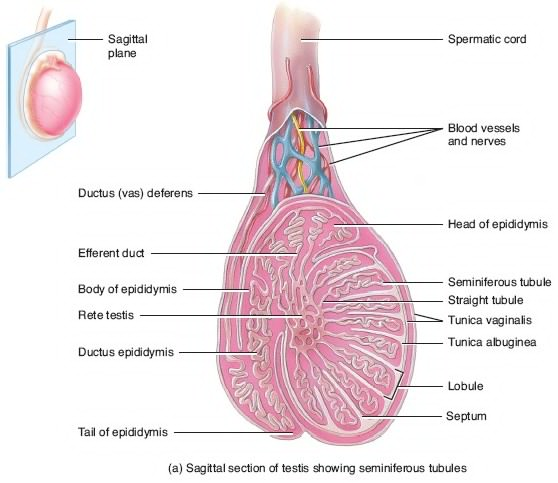
\includegraphics[scale=0.65]{figure/coupe_testicule2} 
  
  }
  
  \caption{Schéma anatomique du testicule humain : }\label{fig:testicule}
  \end{figure}
  
  \subsection{La phase de
  multiplication}\label{la-phase-de-multiplication}
  
  La phase de multiplication est la phase au cours de laquelle les
  spermatogonies se divisent par mitoses pour aboutir au stade de
  spermatocytes primaires. Les spermatogonies sont des cellules diploïdes
  à l'origine de l'ensemble des autres cellules germinales humaines. Pour
  cela, elles vont s'auto-renouveler par mitose successive afin de
  maintenir une production continue de spermatozoïdes tout au long de la
  vie de l'individu. Ces cellules sont localisées dans le compartiment
  basal des tubes séminifères. Les analyses histologiques ont permis de
  distinguer trois types de spermatogonies en fonction de leur contenu en
  hétérochromatine (Clermont, \protect\hyperlink{ref-Clermont1963}{1963},
  Clermont (\protect\hyperlink{ref-Clermont1966}{1966}), Goossens \&
  Tournaye (\protect\hyperlink{ref-Goossens2013}{2013})) :
  
  \begin{enumerate}
  \def\labelenumi{\arabic{enumi}.}
  \tightlist
  \item
    Les spermatogonies de type A dark (ou Ad)\\
  \item
    Les spermatogonies de type A pale (ou Ap)\\
  \item
    Les spermatogonies de type B
  \end{enumerate}
  
  Chez l'Homme, les spermatogonies Ad ont une activité mitotique au cours
  de la spermatogénèse et servent de réserve. Elles vont au cours d'une
  première mitose former une spermatogonie Ad et un spermatogonie Ap
  (\textbf{Figure :} \ref{fig:spermatogenese}). Cette propriété permet à
  la fois de se différencier en spermatocytes tout en constituant un
  compartiment de réserve de spermatogonies Ad pour la régénération de la
  population de cellules germinales au sein de l'épithélium séminifère.
  L'entrée en division des spermatogonies Ap se fait par groupes
  cellulaire tous les 16 jours. Les cellules d'une même génération
  maintiennent entre elles des ponts cytoplasmiques jusqu'à la
  \protect\hyperlink{spermiogenese}{spermiogénèse} ce qui permet la
  synchronisation parfaite du développement gamétique de toutes les
  cellules filles issues d'un groupe de spermatogonies Ap. Ce phénomène
  est appelé onde spermatogénétique. Chaque spermatogonie Ap va,
  lorsqu'elle se divise par mitose, former deux spermatogonies B qui
  elles-mêmes se diviseront en deux spermatocytes primaires diploïdes
  (\textbf{Figure :} \ref{fig:spermatogenese}).
  
  \begin{figure}
  
  {\centering 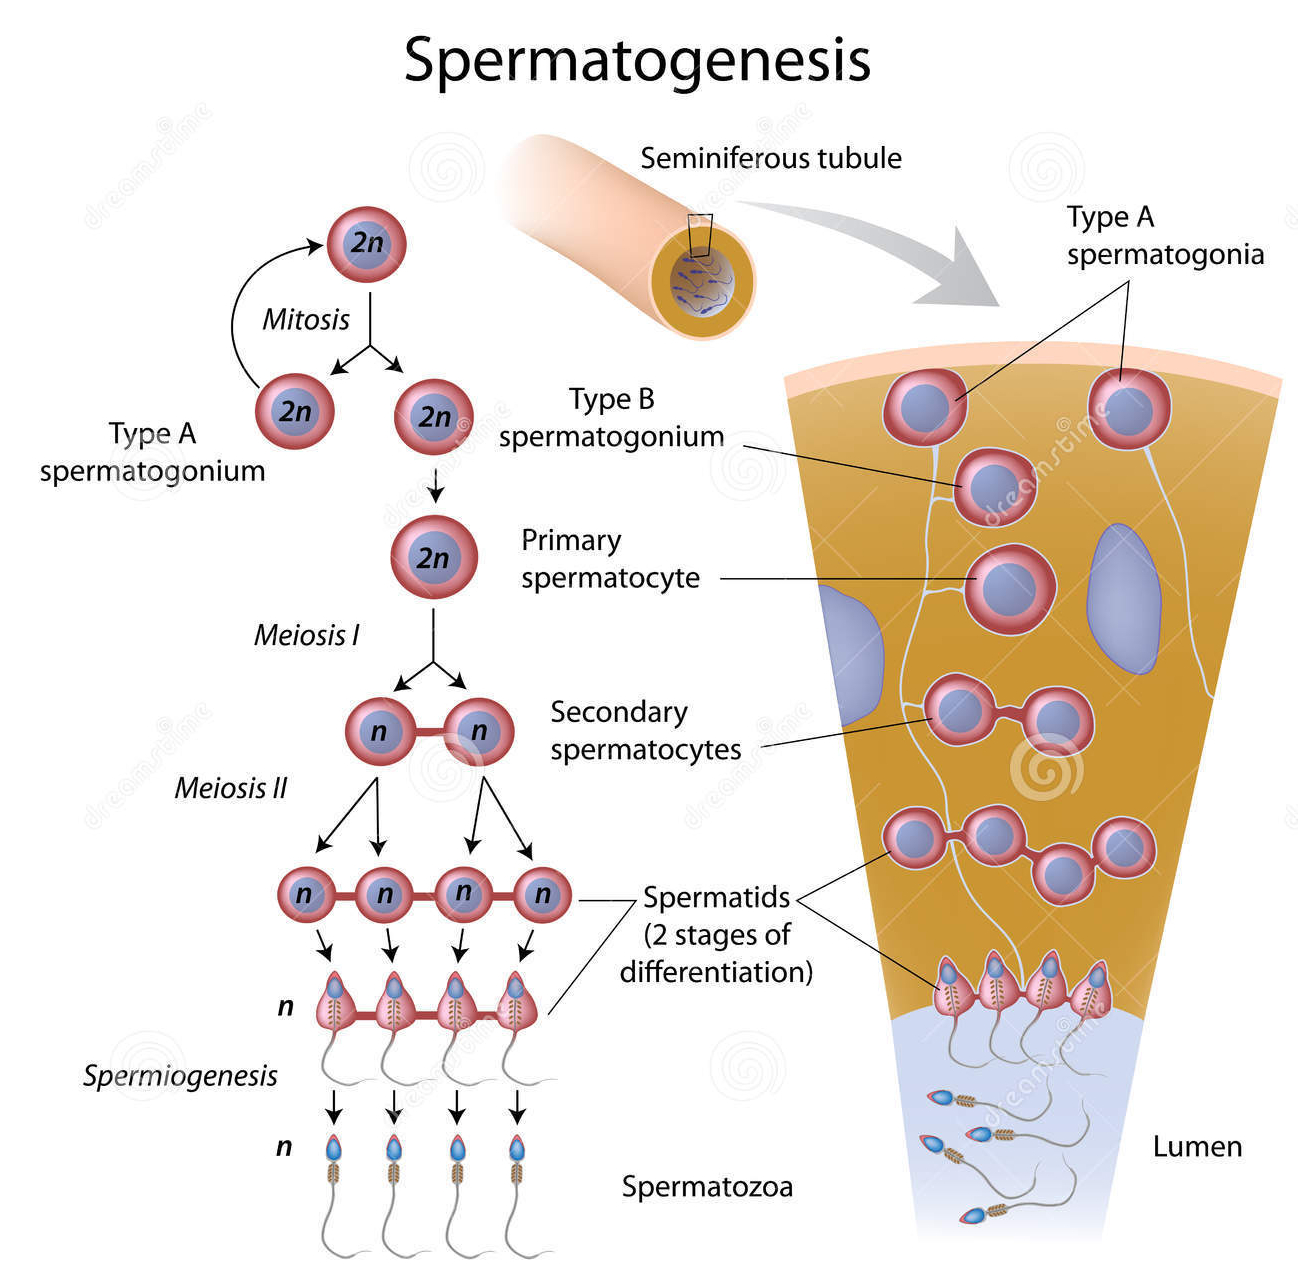
\includegraphics[scale=0.35]{figure/spermatogenese2} 
  
  }
  
  \caption{Les différentes phases de la spermatogénèse d'après [medizin-kompakt](http://www.medizin-kompakt.de/spermatogenese) : description à écrire !!!}\label{fig:spermatogenese}
  \end{figure}
  
  \hypertarget{meiose}{\subsection{La méiose}\label{meiose}}
  
  La méiose, ou phase de maturation, est l'étape au cours de laquelle, à
  partir de cellules diploïdes (les spermatogonies B) vont se former des
  cellules haploïdes, les spermatocytes secondaire (spermatocytes II). Ce
  résultat est le fruit de deux divisions successives (\textbf{Figure :
  }\ref{fig:meiose}) appelée respectivement méiose réductionnelle ou
  méiose I (MI) et méiose équationnelle ou méiose II (MII). La MI va
  séparer les chromosomes homologues, produisant deux cellules et
  réduisant la ploïdie de diploïde à haploïde (d'où son non
  \emph{réductionnelle}). En plus de son rôle de division vu précédemment,
  la méiose joue un rôle clef dans le brassage génétique (mélange des
  gènes) et ce, grâce à deux mécanismes de brassage : le brassage
  inter-chromosomique, lorsque les chromosomes sont séparés et le brassage
  intra-chromosomique impliquant notamment des enjambements chromosomiques
  (crossing-over) (\textbf{Figure : }\ref{fig:crossingover}).
  
  \begin{figure}
  
  {\centering 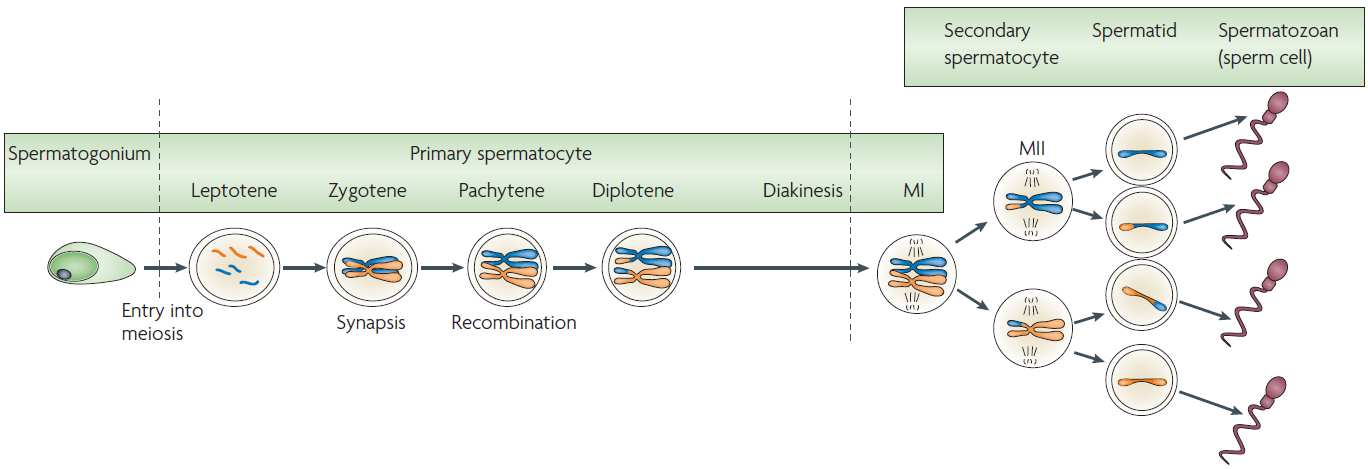
\includegraphics[scale=0.33]{figure/Meiosis_Stages} 
  
  }
  
  \caption[Les différentes étapes de la méiose gamétique masculine]{Les différentes étapes de la méiose gamétique masculine d'après Sasaki et Matsui, 2008}\label{fig:meiose}
  \end{figure}
  
  La méiose est initiée dès la fin de la phase de multiplication à partir
  des spermatocytes primaires issus de la division des spermatogonies de
  type B. Ces cellules nouvellement formées se situent dans le
  compartiment basal du tube séminifère. C'est là qu'ils vont tout d'abord
  subir une interphase (stade préleptotène) durant entre 2 à 4 jours. Au
  cours de cette phase a lieu la réplication de l'ADN. Cette réplication
  se fait lorsque l'ADN est à l'état de chromatine, pendant la phase S
  (pour synthèse) de l'interphase. À l'issue de cette phase, chaque
  chromosome sera composé de deux chromatides reliés entre elles par le
  centromère, le matériel génétique de chaque cellule ayant donc été
  multiplié par 2. Par la suite, ces cellules vont subir deux divisions
  méiotiques, chacune composées de 4 étapes distincte (\textbf{Figure :
  }\ref{fig:meiose}) :
  
  \begin{enumerate}
  \def\labelenumi{\arabic{enumi}.}
  \tightlist
  \item
    \textbf{Méiose réductionnelle} : (\textbf{Figure : }\ref{fig:meiosei})
  
    \begin{enumerate}
    \def\labelenumii{\alph{enumii}.}
    \tightlist
    \item
      \textbf{La prophase I} : Cette longue étape dure 23 jours chez
      l'homme et peut être subdivisée en 5 phases successives : leptotène,
      zygotène, pachytène, diplotène et diacinèse.
  
      \begin{enumerate}
      \def\labelenumiii{\roman{enumiii}.}
      \tightlist
      \item
        \textbf{Leptotène} : condensation de la chromatine et formation
        des chromosomes.\\
      \item
        \textbf{Zygotène} : Appariement des chromosomes homologues par
        paires appelées bivalents grâce l'intermédiaire d'une structure
        multi-protéique : le complexe synaptonémal.\\
      \item
        \textbf{Pachytène} : Ce stade dure 16 jours et est le plus long de
        la prophase I. C'est au cours de celui-ci qu'à lieu l'échange de
        matériel génétique par le biais des crossing-over (\textbf{Figure
        : }\ref{fig:crossingover}) entre les chromatides non-sœurs appelés
        nodules de recombinaison.\\
      \item
        \textbf{Diplotène} : La dissociation du complexe synaptonémal va
        permettre aux chromosomes homologues d'initier leur séparation.
        Certains sites d'appariement étroits nommés chiasmas demeurent
        néanmoins permettant une séparation plus progressive des
        chromosomes et réduisant ainsi le risque d'aneuploïdies (nombre
        anormal de chromosomes) (Handyside,
        \protect\hyperlink{ref-Handyside2012}{2012}).\\
      \item
        \textbf{Diacinèse} : Cette étape marque la fin de la méiose I et
        fait office de transition avec la méiose II. Elle est caractérisée
        par une condensation maximale des chromosomes et la disparition de
        la membrane nucléaire et du nucléole. Le fuseau méiotique commence
        à s'assembler, les centromères des chromosomes homologues
        s'éloignent et les chiasmas glissent progressivement vers les
        télomères.\\
      \end{enumerate}
    \item
      \textbf{La métaphase I} : phase au cours de laquelle les chromosomes
      vont s'aligner à l'équateur de la cellule pour former la plaque
      équatoriale.
    \item
      \textbf{L'anaphase I} : les chromatides sœurs (ou les chromosomes
      homologues en fonction de la phase méiotique) vont se séparer et
      migrer aux pôles opposés de la cellule.\\
    \item
      \textbf{La télophase I} : qui est l'étape finale, les chromosomes se
      décondensent et l'enveloppe nucléaire se reforme autours des
      chromosomes. La cellule mère se sépare alors en deux cellules filles
      appelées spermatocytes secondaires.
    \end{enumerate}
  \end{enumerate}
  
  \begin{figure}
  
  {\centering 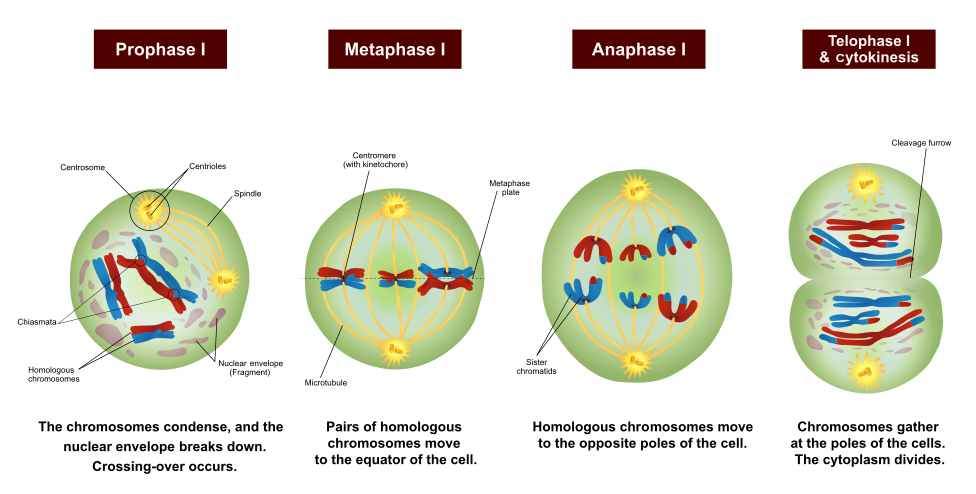
\includegraphics[scale=0.43]{figure/MeiosisI} 
  
  }
  
  \caption[Les différentes étapes de la première division méiotique masculine adapté]{Les différentes étapes de la première division méiotique masculine adapté d'après [Wikipédia](https://en.wikipedia.org/wiki/Meiosis)}\label{fig:meiosei}
  \end{figure}
  
  \begin{enumerate}
  \def\labelenumi{\arabic{enumi}.}
  \setcounter{enumi}{1}
  \tightlist
  \item
    \textbf{Méiose équationnelle} : (\textbf{Figure : }\ref{fig:meioseii})
    La MII est similaire à une division mitotique,
  
    \begin{enumerate}
    \def\labelenumii{\alph{enumii}.}
    \tightlist
    \item
      \textbf{La prophase II} : Contrairement à la prophase I, la prophase
      II est très courte. Les chromosomes, alors formés de deux
      chromatides sœurs se dirigent vers la plaque équatoriale.\\
    \item
      \textbf{La métaphase II} : À ce stade, les chromosomes sont alignés
      le long de la plaque équatoriale au niveau de leur centromère.\\
    \item
      \textbf{L'anaphase II} : Les centromère de chaque chromosome se
      rompent permettant aux chromatides sœurs de se diriger vers les
      pôles opposés des spermatocytes II.\\
    \item
      \textbf{La télophase II} : Comme en télophase I, les cellules mères
      se séparent en deux cellules filles haploïdes appelées spermatides,
      contenant chacune n chromosomes.
    \end{enumerate}
  \end{enumerate}
  
  \begin{figure}
  
  {\centering 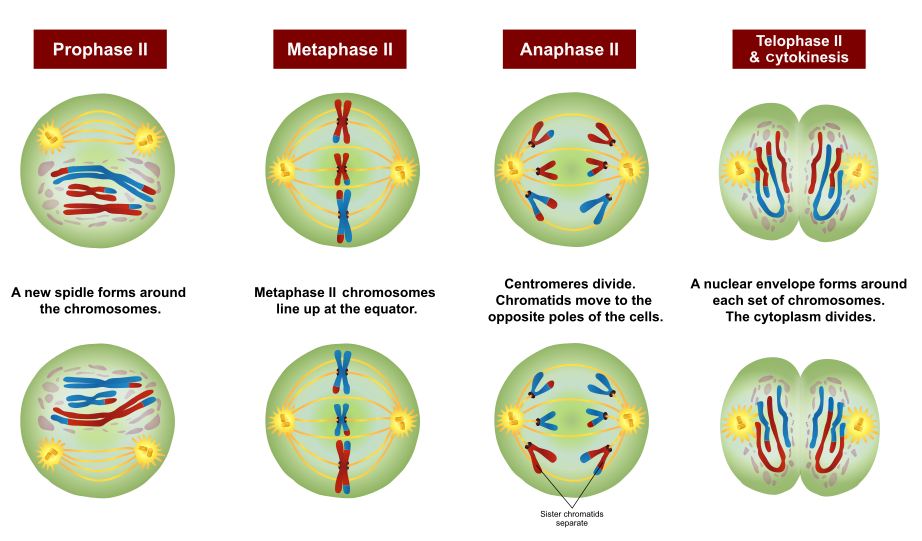
\includegraphics[scale=0.43]{figure/MeiosisII} 
  
  }
  
  \caption[Les différentes étapes de la deuxième division méiotique masculine adapté]{Les différentes étapes de la deuxième division méiotique masculine adapté d'après [Wikipédia](https://en.wikipedia.org/wiki/Meiosis)}\label{fig:meioseii}
  \end{figure}
  
  La première division méiotique aboutit à la formation des spermatocytes
  secondaires (spermatocytes II). À ce stade, les cellules sont haploïdes
  et chaque chromosome est composé de deux chromatides sœurs. Après, cette
  brève étape (environ 1 jour) ainsi qu'une très courte interphase sans
  réplication de l'ADN, les spermatocytes II vont entrer en deuxième
  division méiotique. Cette deuxième division est très semblable à une
  division mitotique. La prophase II, à la différence de la prophase I,
  est très courte. Lors de cette étape, les chromosomes constitués de
  chromatides sœurs se dirigent vers la plaque équatoriale. En métaphase
  II, les chromosomes s'alignent au niveau de leurs centromères. En
  anaphase II, les chromatides sœurs se séparent l'une de l'autre et
  migrent vers les pôles opposés des spermatocytes II. Lors de la
  télophase II, on observe la formation de cellules filles haploïdes
  appelées spermatides, contenant chacune n chromosomes.
  
  \begin{figure}
  
  {\centering 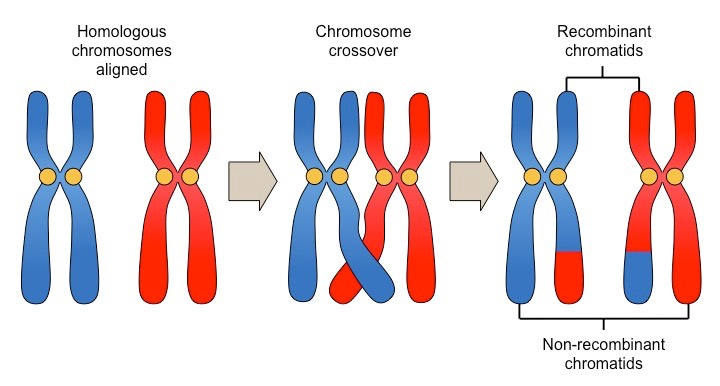
\includegraphics[scale=0.35]{figure/crossingover} 
  
  }
  
  \caption{Schéma simplifié d'un enjambement chromosomique}\label{fig:crossingover}
  \end{figure}
  
  \hypertarget{spermiogenese}{\subsection{La
  spermiogénèse}\label{spermiogenese}}
  
  La spermiogénèse est la phase finale de la spermatogénèse. Elle dure
  environs 23 jours chez l'humain et peut être subdivisée en sept étapes
  (\textbf{Figure : }\ref{fig:spermiogenese}). La spermiogénèse définie la
  cytodiférentiation des spermatides en spermatozoïdes. C'est au cours de
  cette phase que les caractéristiques morphologique et fonctionnelles du
  spermatozoïde seront déterminées (Clermont \& Oko 1993 à trouver !!!).
  Elle est caractérisée par 3 évènements majeurs : la formation de
  l'acrosome, la compaction de l'ADN nucléaire et la formation du
  flagelle. Le développement de l'acrosome et la formation du flagelle
  commence au niveau des spermatides rondes (D. Escalier et al.,
  \protect\hyperlink{ref-Escalier1991}{1991}). Pendant l'élongation de la
  spermatide, le noyau se condense et devient hautement polarisé
  (Hamilton, D. W., Waites, \protect\hyperlink{ref-Hamilton1987}{1990}).\\
  Les spermatides sont situées dans le compartiment adluminal, à proximité
  de la lumière du tube séminifère. Ce sont de petites cellules (8 à 10
  \(\upmu\)m) que l'on peut schématiquement diviser en trois classes :
  
  \begin{enumerate}
  \def\labelenumi{\arabic{enumi}.}
  \tightlist
  \item
    \textbf{Les spermatides rondes} (\textbf{Figure :
    }\ref{fig:spermiogenese} 1-2) : L'identification de ces cellules
    représente une difficulté technique. Elles ont cependant pu être
    décrites en détail par différentes techniques de coloration sous
    microscope optique (Clermont,
    \protect\hyperlink{ref-Clermont1963}{1963}, Papic, Katona, \& Skrabalo
    (\protect\hyperlink{ref-Papic}{1988}), Schenck \& Schill (n.d.),
    Adelman \& Cahill (\protect\hyperlink{ref-Adelman1989}{1989}), World
    Health Organization
    (\protect\hyperlink{ref-WorldHealthOrganization1992}{1992})).
    Plusieurs études animales ont pu démontrées le potentiel des
    spermatides rondes à donner la vie à des individus sains et fertiles,
    (a Ogura, Matsuda, \& Yanagimachi,
    \protect\hyperlink{ref-Ogura1994}{1994}), A. Ogura, Matsuda, Asano,
    Suzuki, \& Yanagimachi (\protect\hyperlink{ref-Kimura1995}{1996}),
    Sasagawa \& Yanagimachi (\protect\hyperlink{ref-Sasagawa}{1997}){]},
    la même chose ayant été également observée plus récemment chez l'homme
    (A. Tanaka et al., \protect\hyperlink{ref-Tanaka2015}{2015}) bien que
    le taux de fécondation et d'implantation soit extrêmement faible
    (Asimakopoulos, \protect\hyperlink{ref-Asimakopoulos2003}{2003}). Ils
    possèdent un noyau rond avec une chromatine pâle et homogène. C'est à
    partir de ces étapes que démarre la biogenèse de l'acrosome avec la
    production par l'appareil de Golgi des vésicules pro-acrosomales
    (phase de Golgi). Les deux centrioles contenus dans le cytoplasme vont
    se déplacer au futur pôle caudal. Le centriole proximal est inactif
    alors que le centriole distal donne naissance à un ensemble de
    microtubules à l'origine de l'axonème du futur flagelle.\\
  \item
    \textbf{Les spermatides en élongation} (\textbf{Figure :
    }\ref{fig:spermiogenese} 3-4) :\\
    peuvent aussi donner naissance avec un meilleur taux que les
    spermatides rondes et engendrerai théoriquement moins de risques
    d'anomalies génétiques ((Asimakopoulos,
    \protect\hyperlink{ref-Asimakopoulos2003}{2003})). \textbf{A
    completer}\\
  \item
    \textbf{Les spermatides en condensation} (\textbf{Figure :
    }\ref{fig:spermiogenese} 5-7) : C'est le stade final de la
    différentiation de la spermatide en spermatozoïde. À ce stade le noyau
    est très allongé, avec une partie caudale globulaire et une partie
    antérieure saillante. La chromatine est sombre et condensée. L'axonème
    va continuer à s'allonger pour former le flagelle mature. Les
    différentes organelles inutiles pour la physiologique spermatique et
    l'excès de cytoplasme vont former la gouttelette cytoplasmique qui va
    se détacher et donner le corps résiduel qui va ensuite être phagocyté
    par les cellules de Sertoli (Hermo, Pelletier, Cyr, \& Smith,
    \protect\hyperlink{ref-Hermo2010}{2010}).
  \end{enumerate}
  
  Une fois ces étapes de différentiation finies, les spermatides sont
  relâchées en tant que spermatozoïdes dans la lumière du tube séminifère.
  Ce procédé est appelé spermiation.
  
  \begin{figure}
  
  {\centering 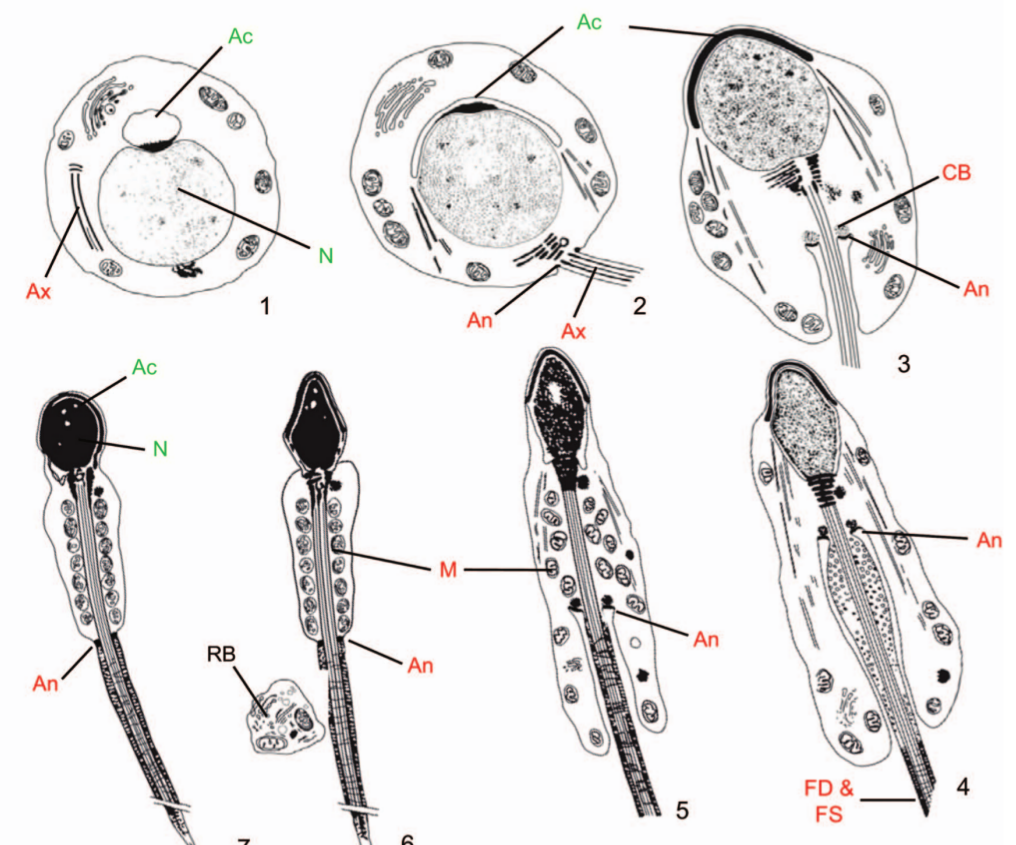
\includegraphics[scale=0.3]{figure/spermiogenese} 
  
  }
  
  \caption[Principales étapes et modifications structurales lors de la spermiogénèse]{Principales étapes et modifications structurales lors de la spermiogénèse d'après Touré et al., 2011 : 1. La spermatide immature avec un gros noyau arrondi. La vésicule acrosomale est attachée au noyau, l’ébauche du flagelle n’atteint pas le noyau. 2. La vésicule acrosomale a augmenté de taille et apparaît aplatie au niveau du noyau. Le flagelle entre en contact avec le noyau. 3-7. Formation de l’acrosome, condensation du noyau et développement des structures flagellaires. Ac, acrosome ; Ax, axonème ; CC, corps chromatoïdes ; CR, corps résiduel ; FD, fibres denses ; GF, gaine fibreuse ; M, mitochondrie ; Ma, manchette. D’après }\label{fig:spermiogenese}
  \end{figure}
  
  \newpage  
  
  \section{Structure et fonction du
  spermatozoïde}\label{structure-et-fonction-du-spermatozoide}
  
  \subsection{Anatomie du spermatozoïde}\label{anatomie-du-spermatozoide}
  
  Le spermatozoïde est une cellule hautement différenciée dont la taille,
  l'orientation et la symétrie sont déterminée. La morphologie générale du
  spermatozoïde éjaculé est similaire à celle du spermatozoïde
  testiculaire. Le spermatozoïde humain normal mature mesure environ 60
  \(\upmu\)m de long et est essentiellement constitué de deux parties : la
  tête et le flagelle (\textbf{Figure : }\ref{fig:spz}).
  
  \begin{figure}
  
  {\centering 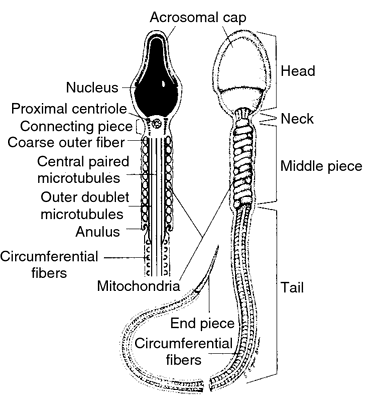
\includegraphics[scale=.75]{figure/sperm_anatomy} 
  
  }
  
  \caption[Anatomie simplifiée du spermatozoïde]{Anatomie simplifiée du spermatozoïde}\label{fig:spz}
  \end{figure}
  
  \subsubsection{La tête}\label{la-tete}
  
  \begin{enumerate}
  \def\labelenumi{\arabic{enumi}.}
  \tightlist
  \item
    \textbf{L'acrosome} : C'est une vésicule de sécrétion géante située
    dans la moitié supérieure de la tête du spermatozoïde. Elle se
    développe à partir de l'appareil de Golgi lors de la spermiogénèse. Au
    cours de sa formation, l'acrosome forme tout d'abord un granule
    sphérique qui se colle sur la partie apicale du noyau. En
    s'aplatissant contre celui-ci, l'acrosome va prendre une forme
    hémisphérique recouvrant la membrane nucléaire formant la coiffe
    céphalique\ldots{} Le rôle de l'acrosome est fondamental dans le
    processus de fécondation puisqu'il permet d'excréter notamment
    l'acrosine, une enzyme de digestion permettant au spermatozoïde de
    pénétrer la zone pellucide qui entoure les ovocytes. Ce processus de
    relargage est appelé réaction acrosomal.\\
  \item
    \textbf{L'acroplaxome} : L'acroplaxome est une structure cytosquelette
    composée de de microfilaments d'actine (F- actine) et de kératine 5.
    Cette structure est positionnée en face de l'appareil de golgi et
    contre le noyau et sert de point d'attachement ainsi que de guide aux
    la vésicules pro-acrosomales (Abraham L Kierszenbaum \& Tres,
    \protect\hyperlink{ref-Kierszenbaum2004}{2004}). C'est une structure
    transitoire qui disparaît remplacée par la thèque périnucléaire dans
    le spermatozoïde mature.\\
  \item
    \textbf{Le noyau} : C'est une structure cellulaire présente dans la
    majorité des cellules eucaryotes. Il contient l'essentiel du matériel
    génétique. Le noyau du spermatozoïde est caractérisé par une
    compaction extrêmement importante de l'ADN. Dans les cellules
    somatiques l'ADN est enroulé par unité de 146 paires de bases autour
    d'un octamère d'histones dit de cœur (H2A, H2B, H3 et H4) afin
    d'organiser les 3 milliards de paires de bases du génome humain dans
    un noyau de quelques microns (\textbf{Figure : }\ref{fig:noyau}).
    L'ADN des spermatides va subir une réorganisation chromatinienne plus
    importante au cours de la spermatogénèse afin d'augmenter sa
    compaction. Ainsi, les octamères d'histones présents dans les cellules
    somatiques sont remplacées par deux protéines riches en arginine et en
    cystéine PRM1 et PRMM2). Ces protéines sont appelées des protamines
    (\textbf{Figure : }\ref{fig:noyau}). L'intégrité des deux protéines
    composant ce dimère est nécessaire pour la procréation (Cho et al.,
    \protect\hyperlink{ref-Cho2001}{2001}). Cette compaction extrême
    permet de réduire la taille du noyau, mais aussi de protéger l'ADN
    d'agents de dégradation comme l'oxydation des bases. Parallèlement à
    cette condensation chromatinienne se produit un arrêt des processus de
    transcription cellulaire (A L Kierszenbaum \& Tres,
    \protect\hyperlink{ref-Kierszenbaum1978}{1978}). Le noyau du
    spermatozoïde est donc un noyau au repos, transcriptionnellement
    inactif (Ward, \protect\hyperlink{ref-Ward1994}{1994})
  \end{enumerate}
  
  \begin{figure}
  
  {\centering 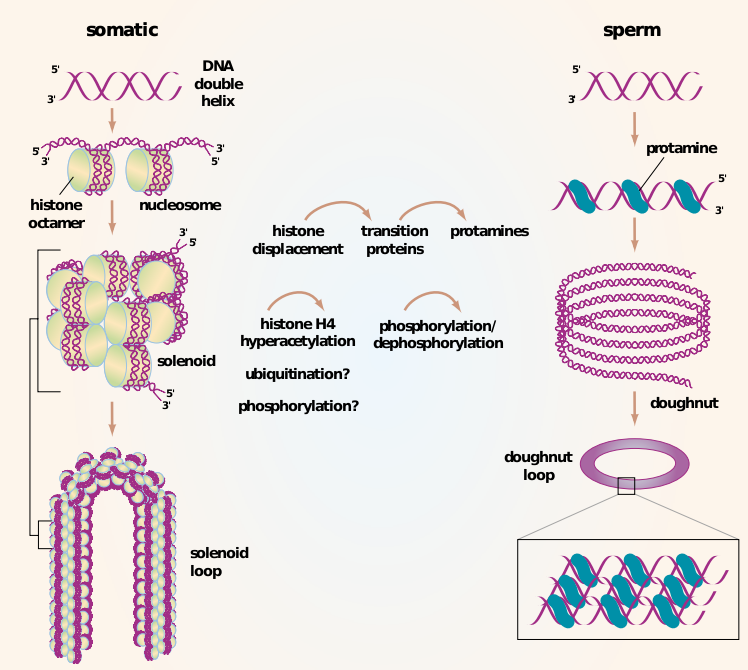
\includegraphics[scale=.55]{figure/noyau} 
  
  }
  
  \caption[Schéma de la compaction de l’ADN dans les cellules somatiques et dans les spermatozoïdes]{Schéma de la compaction de l’ADN dans les cellules somatiques et dans les spermatozoïdes : D'après Braun (2001)}\label{fig:noyau}
  \end{figure}
  
  \subsubsection{Le flagelle}\label{le-flagelle}
  
  Le flagelle représente la queue du spermatozoïde. Celui-ci permet, par
  mouvement d'oscillation à haute vitesse, le déplacement du
  spermatozoïde. Cette mobilité est générée par un cytosquelette interne
  extrêmement conservé durant l'évolution appelée l'axonème. Celui-ci est
  composé de neuf doublets de microtubules périphériques et de deux
  doublets internes (Inaba, \protect\hyperlink{ref-Inaba2003}{2003})
  (\textbf{Figure : }\ref{fig:axoneme}), on parle alors de structure ``9 +
  2''. Les doublets externes sont reliés entre eux par des ponts de nexine
  et au doublet central par des ponts radiaires.
  
  \begin{figure}
  
  {\centering 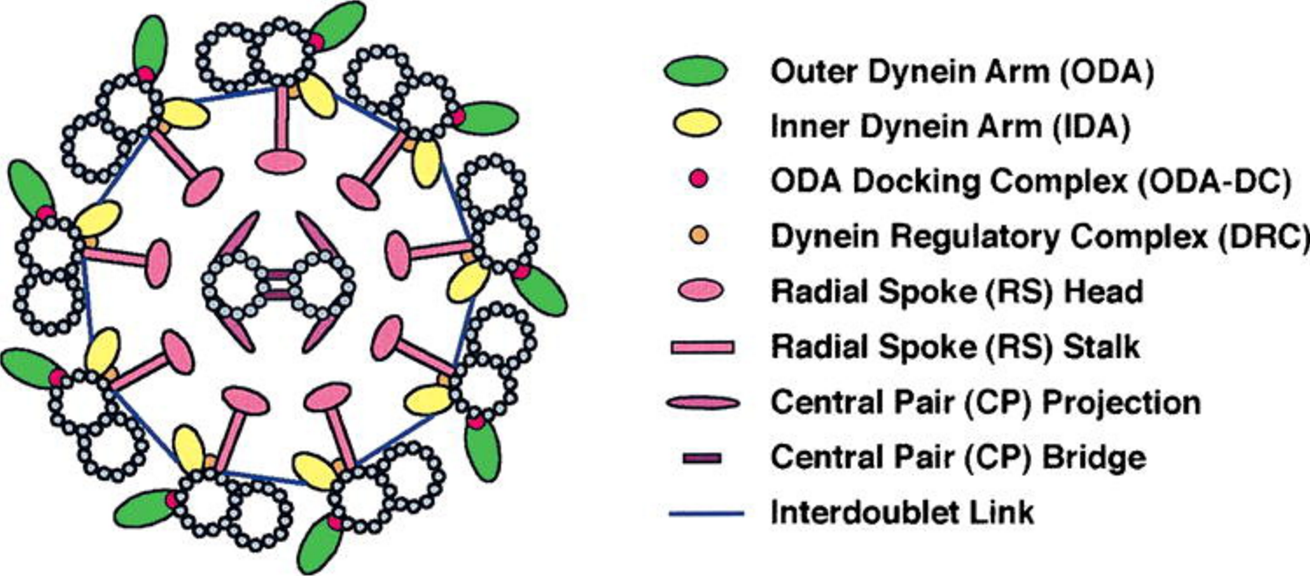
\includegraphics[scale=.3]{figure/axoneme} 
  
  }
  
  \caption[Structure simplifiée de l'axonème]{Structure simplifiée de l'axonème d'après [@Inaba2003] : L'axonème es constitué de neuf doublets de microtubules périphériques reliés entre eux par des liens de nexine d'un doublet central relié aux doublets périphériques par des ponts radiaires}\label{fig:axoneme}
  \end{figure}
  
  Le flagelle su spermatozoïde peut être divisé en trois partie distinctes
  (\textbf{Figure : }\ref{fig:flagelle}) :
  
  \begin{enumerate}
  \def\labelenumi{\arabic{enumi}.}
  \tightlist
  \item
    \textbf{La pièce intermédiaire} : Elle fait jonction avec la tête du
    spermatozoïde et est composée de la gaine de mitochondrie qui fournira
    une partie de de l'énergie nécessaire au battement flagellaire (grâce
    à la phosphorylation oxydative qui produit de l'ATP), l'axonème qui se
    prolonge dans la pièce principale et un ensemble de neuf faisceaux de
    fibres denses.\\
  \item
    \textbf{La pièce principale} : Ici, la gaine de mitochondrie a
    disparue ainsi que deux des faisceaux de fibres denses présents dans
    la pièce intermédiaire. On note cependant la présence d'une structure
    supplémentaire, la gaine fibreuse. Cette gaine entoure l'axonème et
    comporte deux épaississements diamétralement opposés, appelées
    colonnes longitudinales sur lesquelles s'insère les fibres denses 3 et
    8. C'est le long de la gaine fibreuse qu'est produit la majorité de
    l'énergie 46nécessaire au glissement des microtubules (Eddy,
    \protect\hyperlink{ref-Eddy2007}{2007}).\\
  \item
    \textbf{La pièce terminale} : Elle est située au niveau de l'extrémité
    distale du flagelle et ne contient que l'axonème (Inaba,
    \protect\hyperlink{ref-Inaba2003}{2003}).
  \end{enumerate}
  
  \begin{figure}
  
  {\centering 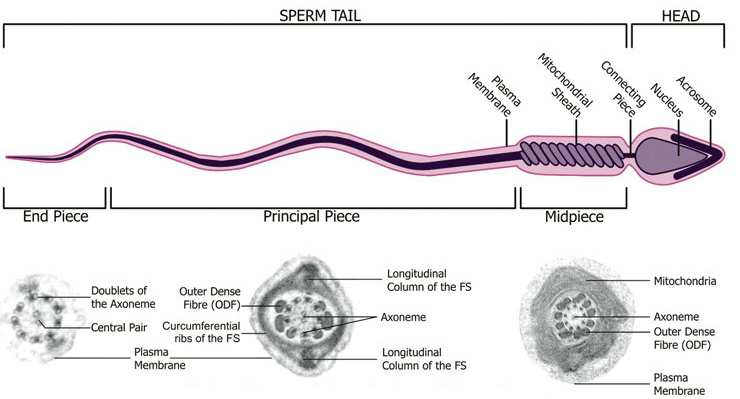
\includegraphics[scale=.55]{figure/sperm2} 
  
  }
  
  \caption[Structure du flagelle d’un spermatozoïde]{Structure du flagelle d’un spermatozoïde d'après Borg et al. (2010) : Coupes transversales en microscopie électronique. Le flagelle se compose de trois parties : la pièce intermédiaire, contenant les mitochondries, la pièce principale et la pièce terminale. L’axonème, en position centrale, parcours tout le flagelle. Des structures périaxonèmales sont observables : les fibres denses dans la pièce intermédiaire et principale, et la gaine fibreuse dans la pièce principale seulement.}\label{fig:flagelle}
  \end{figure}
  
  \subsection{Fonction du spermatozoïde}\label{fonction-du-spermatozoide}
  
  En plus d'être unique dans sa morphologie, le spermatozoïde l'est aussi
  dans sa fonction puisque c'est la seule cellule produite de manière
  endogène et dont l'action est exercée de manière exogène.
  
  \newpage  
  
  \section{L'infertilité masculine}\label{linfertilite-masculine}
  
  L'organisation mondiale de la santé définie l'infertilité comme étant :
  ``\emph{une pathologie du système reproductif définie par l'échec d'une
  grossesse clinique après 12 mois ou plus de rapports sexuels réguliers
  non protégés}''
  (\href{http://www.who.int/reproductivehealth/topics/infertility/definitions/en/}{\texttt{Who.int.\ 2013-03-19.\ Retrieved\ 2013-06-17}}).
  L'étude de l'infertilité représente un des enjeux scientifique et
  médicale majeur de ces dernières années. On estime qu'environ 10 à 15\%
  des couples humains font face à des problèmes d'infertilité soit plus de
  70 millions de personnes dans le monde (Boivin, Bunting, Collins, \&
  Nygren, \protect\hyperlink{ref-Boivin2007a}{2007}). Dans la moitié des
  cas, la cause sous-jacente serait masculine. On estime que Les facteurs
  causaux sous-jacents de l'infertilité masculine peuvent être attribués à
  des toxines environnementales, des troubles systémiques tels que la
  maladie hypothalamo-hypophysaire, les cancers testiculaires et l'aplasie
  des cellules germinales. Les facteurs génétiques, y compris les
  aneuploïdies et les mutations de gènes uniques, contribuent également à
  l'infertilité masculine. Cependant, aucune cause n'est identifiée dans
  10-20\% des cas. Comme nous avons pu le voir, la spermatogénèse est une
  succession de processus complexes qui s'effectue de manière synchrone,
  de fait la moindre altération génétique affectant une seule de ces
  étapes est susceptible d'entrainer un phénotype d'infertilité (Barratt,
  1995 \textbf{A TROUVER}).
  
  \subsection{Les différents phénotypes d'infertilité
  masculine}\label{les-differents-phenotypes-dinfertilite-masculine}
  
  Chez l'homme, l'infertilité est associée à une altération quantitative
  et / ou qualitative des spermatozoïdes présents dans l'éjaculat.
  L'ensemble de ces altérations peuvent être détectées et quantifiées dans
  des laboratoires spécialisés par réalisation d'un spermogramme. Au cours
  de celui-ci, plusieurs critères tel que le volume de sperme sécrété, son
  pH, la quantité et la vitalité des spermatozoïdes qu'il contient seront
  évalués. La proportion de cellules immatures sera elle aussi analysée.
  Ces cellules épithéliales de l'urètre, appelées aussi cellules rondes,
  se retrouvent à la fois dans l'éjaculat des individus ayant une quantité
  de spermatozoïdes ``normal'' (Michael \& Joel,
  \protect\hyperlink{ref-Michael1937}{1937},M. Tomlinson et al.
  (\protect\hyperlink{ref-Tomlinson1993a}{1993})), chez les individus
  présentant une quantité basse de spermatozoïdes (MacLeod,
  \protect\hyperlink{ref-MacLeod1970}{1970}, M. J. Tomlinson, Barratt, \&
  Cooke (\protect\hyperlink{ref-Tomlinson1993}{1993})) ou en étant
  dépourvu (Kurilo, Liubashevskaia, Dubinskaia, \& Gaeva,
  \protect\hyperlink{ref-Kurilo}{1993}). Cependant, leur nombre augmente
  tandis que la quantité de spermatozoïde diminu (SPERLING \& KADEN,
  \protect\hyperlink{ref-SPERLING1971}{1971}).
  
  \subsubsection{Liée à la quantité}\label{liee-a-la-quantite}
  
  Chez l'humain, l'arrêt de la spermatogénèse est défini comme
  l'incapacité des cellules spermatogénétique à devenir des spermatozoïdes
  matures. Elle peut survenir à n'importe qu'elle étape de la formation
  des cellules germinales. Les arrêts au stade de spermatocyte I sont les
  plus fréquents, suivis par l'arrêt au niveau des spermatides et moins
  fréquemment au niveau des spermatogonies (Girgis, Etriby, Ibrahim, \&
  Kahil, \protect\hyperlink{ref-Girgis}{1969}).
  
  \begin{enumerate}
  \def\labelenumi{\arabic{enumi}.}
  \tightlist
  \item
    \textbf{L'oligozoospermie} : L'oligozoospermie est définie comme un
    phénotype d'infertilité masculine caractérisé par une production
    inférieure à 15 millions de spermatozoïdes par ml de sperme (T. G.
    Cooper et al., \protect\hyperlink{ref-Cooper2010}{2010}). Un arrêt de
    la spermatogénèse a été observée dans 4 à 30\% des biopsie
    testiculaire des hommes présentant une oligospermie sévère (Colgan,
    Bedard, Strawbridge, Buckspan, \& Klotz,
    \protect\hyperlink{ref-Colgan1980}{1980}, Levin
    (\protect\hyperlink{ref-Levin1979}{1979}), Soderström \& Suominen
    (\protect\hyperlink{ref-Soderstrom1980}{1980}), WONG, STRAUS, \&
    WARNER (\protect\hyperlink{ref-WONG1973}{1973})). Cet arrêt a
    longtemps été considérés comme sans espoir pour les couples désirant
    concevoir, jusqu'à l'émergence de \emph{intracytoplasmic sperm
    injection} (ICIS) (Palermo, Joris, Devroey, \& Van Steirteghem,
    \protect\hyperlink{ref-Palermo1992}{1992})\\
  \item
    \textbf{L'azoospermie} : Comme l'oligozoospermie, l'azoospermie est un
    phénotype d'infertilité masculine cette fois-ci caractérisé par
    l'absence total de spermatozoïde dans l'éjaculat. On distingue des
    causes excrétoires empêchant l'excrétion des spermatozoïdes, on parle
    alors d'azoospermie obstructive et des causes sécrétoires, les plus
    fréquentes, accompagnées d'un défaut de la spermatogenèse, on parle
    alors d'azoospermie non-obstructive.
  \end{enumerate}
  
  \subsubsection{Liée à la morphologie}\label{liee-a-la-morphologie}
  
  Ces anomalies sont observables en effectuant un spermocytogramme.
  Plusieurs classifications ont été établie, cependant, c'est la
  classification de David modifiée (\textbf{Table :}
  \ref{fig:anomaliemorphosperm}) qui est la plus rependue en France. Pour
  ce faire, on procède généralement à une observation de 100
  spermatozoïdes au cours de laquelle l'ensemble des anomalies observées
  sont relevées et quantifiées permettant ainsi de définir un index
  d'anomalies multiple (nombre total d'anomalies/nombre de spermatozoïdes
  anormaux) révélant le nombre moyen d'anomalies par spermatozoïdes.
  
  \begin{figure}
  
  {\centering 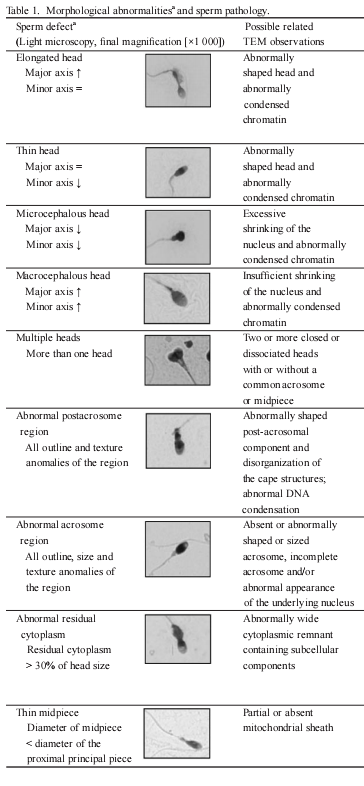
\includegraphics[scale=.75]{figure/sperm_morpho_abnormalities} 
  
  }
  
  \caption[Différentes anomalies morphologiques du spermatozoïde selon la classification de David modifiée adapté... TABLEAU à adapter et à insérer !!!!!]{Différentes anomalies morphologiques du spermatozoïde selon la classification de David modifiée adapté... TABLEAU à adapter et à insérer !!!!! d'après [@Auger2010]}\label{fig:anomaliemorphosperm}
  \end{figure}
  
  \subsubsection{Liée à la mobilité}\label{liee-a-la-mobilite}
  
  Le succès du passage du spermatozoïdes le long du tractus génitale
  féminin dépend en grande partie de la mobilité et de la vitesse du
  spermatozoïde (Lindholmer, \protect\hyperlink{ref-Lindholmer1974}{1974},
  Björndahl (\protect\hyperlink{ref-Bjorndahl2010}{2010})). La vitesse
  moyenne d'un spermatozoïde étant de 25 \(\upmu\)m/s. Une mauvaise
  mobilité observée dans plus de 50\% des spermatozoïdes éjaculés se
  révèle être un prédicteur de l'échec de la fécondation (Aitken, Sutton,
  Warner, \& Richardson, \protect\hyperlink{ref-Aitken1985}{1985}).
  
  \subsection{La génétique de
  l'infertilité}\label{la-genetique-de-linfertilite}
  
  Comme il a déjà été dit, il est estimé que 10 à 15\% des couples humain
  font face à des problèmes d'infertilité. Par ailleurs, 30\% des
  infertilités restent inexpliquées et près de 40\% ont des causes
  incertaines. Ainsi, l'infertilité masculine d'origine génétique pourrait
  concerner près de 1 homme sur 40 (Tüttelmann et al.,
  \protect\hyperlink{ref-Tuttelmann2011}{2011}).
  
  \subsubsection{Les causes fréquentes}\label{les-causes-frequentes}
  
  \begin{enumerate}
  \def\labelenumi{\arabic{enumi}.}
  \tightlist
  \item
    \textbf{Les microdélétions du chromosome Y} : Le chromosome Y est un
    petit chromosome atteignant une taille d'environ 53 Mb et est porteur
    de 78 gènes principalement impliqués dans la différentiation sexuelle
    masculine et la spermatogénèse (Skaletsky et al.,
    \protect\hyperlink{ref-Skaletsky2003}{2003}). De fait, le chromosome Y
    représente une région d'intérêt évidente dans l'étude de facteur
    génétique liés à l'infertilité masculine. L'évolution des technologies
    a permis de mettre en évidence des délétion invisibles au caryotype
    dans la région du facteur AZF (\emph{Azoospermia Factor}). Cette
    région peut être subdivisée en trois sous-partie, AZFa, AZFb et AZFc
    (\textbf{Figure :} \ref{fig:chry}). Depuis plusieurs années, de
    nombreuses séries de patients azoospermiques ou oligozoospermiques ont
    été publiées et tendent à montrer que les microdélétions du chromosome
    Y seraient responsables de 10\% des cas d'azoospermie non-obstructives
    et chez 5\% des cas d'oligozoospermie sévères (\textless{}5 millions
    de spermatozoïdes/ml) (Hotaling \& Carrell,
    \protect\hyperlink{ref-Hotaling2014}{2014}).
  \end{enumerate}
  
  \begin{figure}
  
  {\centering 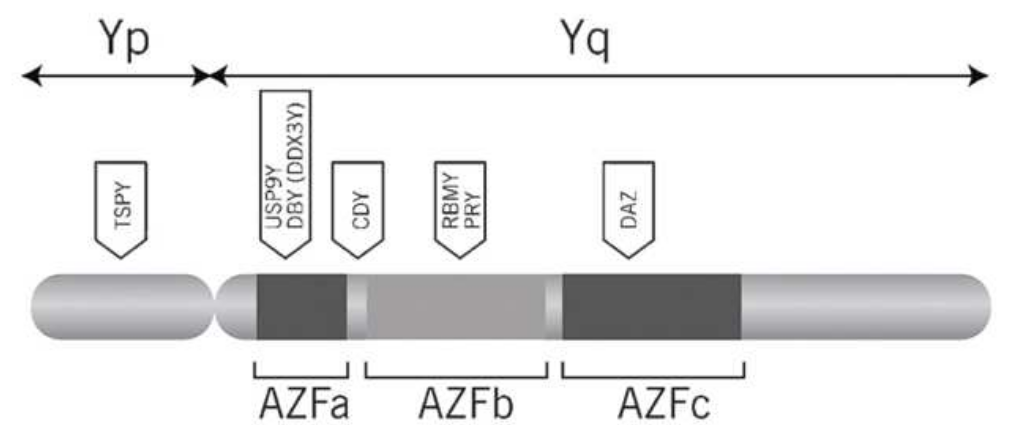
\includegraphics[scale=.45]{figure/chromozomeY} 
  
  }
  
  \caption[Représentation schématique du chromosome Y adapté]{Représentation schématique du chromosome Y adapté d'après [@OFlynnOBrien2010] : Visualisation la région AZF ainsi que des trois sous-régions AZF a, b, c et des principaux gènes compris dans chacune des sous-régions}\label{fig:chry}
  \end{figure}
  
  \begin{enumerate}
  \def\labelenumi{\arabic{enumi}.}
  \setcounter{enumi}{1}
  \tightlist
  \item
    \textbf{Anomalies chromosomiques} : Des anomalies chromosomique de
    nombre ou de structure impliquant les autosomes ou, le plus souvent,
    les gonosomes, peuvent être impliqués dans des cas d'infertilité
    masculine. Le pourcentage d'individu concerné varie entre 2 et 8\% et
    peut atteindre 15\% pour les patients azoospermiques soit 10 à 20 fois
    la fréquence retrouvée dans la population générale (Ravel, Berthaut,
    Bresson, Siffroi, \& Genetics Commission of the French Federation of
    CECOS, \protect\hyperlink{ref-Ravel2006}{2006}).
  
    \begin{enumerate}
    \def\labelenumii{\alph{enumii}.}
    \tightlist
    \item
      \textbf{Syndrome de Klinefelter} : Le syndrome de Klinefelter (ou
      46, XXY) fut décrit pour la première fois en 1942 par Harry F.
      Klinefelter et décrit une affection due à la présence d'un
      chromosome X supplémentaire suite à une erreur de ségrégation des
      chromosomes au moment de la méiose. Sa prévalence dans la population
      générale est estimée à environ 1 sur 1200 (1 homme sur 600) (Bojesen
      \& Gravholt, \protect\hyperlink{ref-Bojesen2011}{2011}) mais elle
      est environs 50 fois supérieure chez les patients infertiles
      azoospermiques (Gekas et al.,
      \protect\hyperlink{ref-Gekas2001}{2001}).\\
    \item
      \textbf{Les anomalies de structure} : Les translocation et les
      inversions sont les anomalies de structures retrouvées le plus
      fréquemment chez les patients infertiles.
  
      \begin{enumerate}
      \def\labelenumiii{\roman{enumiii}.}
      \tightlist
      \item
        La translocation est définie comme l'échange de matériel génétique
        entre deux chromosomes non homologues. On en distingue deux types,
        les translocation réciproques et les translocation
        robertsonniennes. Les premières sont retrouvées 4 à 10 fois plus
        fréquemment chez les patients infertiles que dans la population
        générale (Elliott \& Cooke,
        \protect\hyperlink{ref-Elliott1997}{1997}), les secondes sont
        retrouvées chez 1.6\% des patients oligozoospermiques et 0.09\%
        des patients azoospermiques (O'Flynn O'Brien, Varghese, \&
        Agarwal, \protect\hyperlink{ref-OFlynnOBrien2010}{2010}).\\
      \item
        Les inversions chromosomiques caractérisent le mécanisme de
        cassure d'un fragment de chromosome suivi de son retournement à
        180° et sa réintégration à la même position. Ces inversions vont
        gêner l'appariement des chromosomes homologues (formation d'une
        boucle d'inversion) pendant la méiose et sont, comme les
        translocations, retrouvées plus fréquemment chez les patients
        infertiles que dans la population générale (Krausz \& Forti,
        \protect\hyperlink{ref-Krausz2000}{2000}).\\
      \end{enumerate}
    \item
      \textbf{Autres anomalies chromosomiques} : Parmi les anomalies de
      structures chromosomique responsables d'infertilité masculine, on
      peut par exemple citer les hommes de formule 46,XX bien qu'elle soit
      moins fréquente que les translocations et les inversions. Ces
      patients sont généralement totalement infertiles et présentent une
      azoospermie par absence des sous- régions AZF a, b et c (Vorona,
      Zitzmann, Gromoll, Schüring, \& Nieschlag,
      \protect\hyperlink{ref-Vorona2007}{2007}) bien qu'ils aient un
      phénotype masculin normal.
    \end{enumerate}
  \item
    \textbf{Mutations du gène \emph{CFTR} }: L'identification du gène
    \emph{CFTR} (\emph{Cystic Fibrosis Transmembrane conductance
    Regulator}) chez les patients atteints de mucoviscidose et présentant
    une agénésie bilatérale des canaux déférents (ABCD) a permis
    d'associer ce gène au phénotype d'azoospermie obstructive. Cette
    malformation serait responsable de 2\% des cas d'infertilité masculine
    et de 25\% des cas d'azoospermie obstructive (J. Yu, Chen, Ni, \& Li,
    \protect\hyperlink{ref-Yu2012}{2012}).
  \end{enumerate}
  
  Bien que la prévalence de ces anomalies génétiques varie en fonction du
  phénotype concerné, il est estimé que ces défauts soient seulement
  retrouvés chez 5\% des cas d'infertilité masculine tout phénotype
  confondus. Cette observation suggère fortement l'implication d'autres
  gènes encore inconnus dans les différents phénotypes d'infertilité
  masculine (\textbf{Nieschlag et al., 2010 A trouver}).
  
  \subsubsection{Les nouveaux gènes}\label{les-nouveaux-genes}
  
  \begin{enumerate}
  \def\labelenumi{\arabic{enumi}.}
  \tightlist
  \item
    \textbf{Les anomalies morphologiques liées à la tête du
    spermatozoïdes} :
  
    \begin{enumerate}
    \def\labelenumii{\alph{enumii}.}
    \tightlist
    \item
      \textbf{La macrozoospermie} : Ce phénotype d'infertilité masculine
      rare est caractérisé par la présence de 100\% des spermatozoïdes de
      l'éjaculat présentant une tête anormalement grosse ainsi que
      plusieurs flagelles. Il fut observé pour la première fois en 1978
      (Nistal, Paniagua, \& Herruzo,
      \protect\hyperlink{ref-Nistal}{1978}), mais ce n'est qu'en 2007
      q'une explication génétique fut enfin trouvée. Une étude portant sur
      14 patients nord Africains a permis d'identifier la délétion
      c144delC du gène \emph{AURKC} (\emph{Aurora kinase C}) comme
      responsable du phénotype de l'ensemble des individus de l'étude
      (Dieterich et al., \protect\hyperlink{ref-Dieterich2007}{2007}).
      Depuis, d'autres études ont permis d'associer d'autre variants sur
      ce même gène à ce phénotype {[}INSERT REF{]}. Des anomalies du gène
      \emph{AURKC} seraient ainsi respondable d'environs 83.7\% des cas
      macrozoospermie chez des patients non apparentés {[}INSERT REF{]}.
      Le gène \emph{AURKC}, étant impliqué dans la méiose, conduit
      lorsqu'il est muté à un dysfonctionement de celle-ci menant à des
      spermatozoïdes polyploïdes, c'est à dire, portant une quantité de
      materiel génétique trop important {[}INSERT REF{]}.\\
    \item
      \textbf{La globozoospermie} : La globozoospermie est aussi un
      phénotype rare d'infertilité dont la prévalence est estimée à de
      0,1\%. Il fut dentifié pour la première fois en 1971 et est
      caractérisé par la présence d'une majorité de spermatozoïde dépourvu
      d'acrosome dans l'éjaculat empechant ainsi le spermatozoïde de
      franchir la zone pellucide de l'ovocyte compremettant ainsi la
      fécondation (A. Dam et al., \protect\hyperlink{ref-Dam2006}{2006},
      C. G. S. Sen, Holstein, \& Schirren
      (\protect\hyperlink{ref-Sen2009}{1971}), A. F. Holstein, Schirren,
      \& Schirren (\protect\hyperlink{ref-Holstein1973}{1973})). En 2007,
      une étude familiale a permis de lier ce phénotype à la mutation
      c.848G\textgreater{}A dans le gène \emph{SPATA16}
      (\emph{spermatogenesis-associated protein 16}) (A. H. Dam et al.,
      \protect\hyperlink{ref-Dam2007a}{2007}) dont la protéine va, au
      cours de la spermatogénèse fusioner avec les vésicules
      proacrosomales pour former l'acrosome (A. H. Dam et al.,
      \protect\hyperlink{ref-Dam2007a}{2007}, L. Lu, Lin, Xu, Zhou, \& Sha
      (\protect\hyperlink{ref-Lu2006}{2006})). Plus tard, en 2011, une
      étude portant sur 20 patients tunisiens permit d'identifier une
      délétion homozygote de 200 kb emportant la totalité du gène
      \emph{DPY19L2} (\emph{Dpy-19 Like 2}) chez 15 des 20 patients
      (Harbuz et al., \protect\hyperlink{ref-Harbuz2011}{2011}). cf
      \protect\hyperlink{globo}{globo}\\
    \item
      \textbf{Spermatozoïdes acéphaliques} : Ce phénotype reporté
      plusieurs fois (Hector E. Chemes \& Rawe,
      \protect\hyperlink{ref-Chemes2010}{2010}, Panidis et al.
      (\protect\hyperlink{ref-Panidis2001}{2001}), H E Chemes et al.
      (\protect\hyperlink{ref-Chemes1987}{1987})) caractérise les patients
      présentant des spermatozoïdes déporvu de tête dans leur éjaculat.
      Une étude récente a put lier ce phénotype à une mutation
      c.824C\textgreater{}T homozygote ainsi qu'à deux variants
      hétérozygotes composites c.1006C\textgreater{}T et
      c.485T\textgreater{}A dans le gène \emph{SUN5} (F. Zhu et al.,
      \protect\hyperlink{ref-Zhu2016}{2016}) qui avait précédement été
      décrit comme localisant à la jonction tête / flagelle du
      spermatozoïde (Yassine et al.,
      \protect\hyperlink{ref-Yassine2015}{2015}).\\
    \end{enumerate}
  \item
    \textbf{Les anomalies liées au flagelle et à la motilité} :\\
  
    \begin{enumerate}
    \def\labelenumii{\alph{enumii}.}
    \tightlist
    \item
      \textbf{Phénotype MMAF} : Le phénotype MMAF (\emph{Multiple
      morphological abnormalities of the sperm flagella}) décrit les
      patients atteints d'asthenozoospermie et et les flagelles
      spermatiques présentent de multiples anomalies morphologiques. Ce
      phénotype a été décrit plusieurs fois dans la literature et revait
      plusieurs formes (C. Coutton, Escoffier, Martinez, Arnoult, \& Ray,
      \protect\hyperlink{ref-Coutton2015}{2015}). Plus précisement , ce
      phénotype décritles asthenozoospermie résultant d'une mosaïque
      d'anormalité morphologiques au niveau du flagelle tel que l'abscence
      total de flagelle, des flagelles enroulés, courts, anguleux\ldots{}
      (C. Coutton et al., \protect\hyperlink{ref-Coutton2015}{2015}, Ben
      Khelifa et al. (\protect\hyperlink{ref-BenKhelifa2014}{2014})).
      Recemment, le gène \emph{DNAH1} (\emph{Dynein Axonemal Heavy Chain
      1}) codant pour une dynéine de la chaine lourde de l'axonème a été
      retrouvé muté chez près d'un patient sur trois dans sa cohorte
      comportant 18 patients (Ben Khelifa et al.,
      \protect\hyperlink{ref-BenKhelifa2014}{2014}). Deux autres études
      ont retrouvée des mutation dans le gène \emph{DNAH1} chez des
      patients venant de Chine, d'Iran et d'Italie, laissant suggérer que
      ce gène est l'un des acteurs majeurs dans le syndrome MMAF (X. Wang
      et al., \protect\hyperlink{ref-Wang2017}{2017}, Amiri-Yekta et al.
      (\protect\hyperlink{ref-Amiri-Yekta2016}{2016})).\\
    \end{enumerate}
  \item
    \textbf{Les échec de fécondation du spermatozoïde} : Au moment de la
    fécondation, l'activation ovocytaire repose sur le relargage par le
    spermatozoïde de ``facteurs spermatiques'' qui déclenchent un signal
    de calcium, constitué d'oscillations Ca\(^{2+}\). Ce processus est
    médié par une protéine spécifique du spermatozoïde : PLC\(\zeta\) 1
    (Nomikos, Kashir, Swann, \& Lai,
    \protect\hyperlink{ref-Nomikos2013}{2013}, Amdani, Jones, \& Coward
    (\protect\hyperlink{ref-Amdani2013}{2013})). Plusieurs cas d'echec
    d'activation ovocitaire ont été liés à l'bscence ou la mauvaise
    localisation de la protéine PLC\(\zeta\) 1 (\emph{phospholipase C Zeta
    1}). Malgré celà, aucune preuve génétique directe n'avait été reporté
    jusque récemment où deux mutations au sein du gène
    \emph{PLC}\(\zeta\)\emph{1} furent retrouvés chez un patient (Heytens
    et al., \protect\hyperlink{ref-Heytens2009}{2009}) et un peu plus tard
    une mutation homozygote chez deux frères consanguins (Escoffier et
    al., \protect\hyperlink{ref-Escoffier2016}{2016}).
  \end{enumerate}
  
  \newpage  
  
  \section{Les techniques d'analyses
  génétiques}\label{les-techniques-danalyses-genetiques}
  
  L'acide désoxyribonucléique (ADN) a été identifié comme étant le porteur
  de l'information génétique par Oswald Theodore Avery en 1944. Sa
  structure en double hélice composée par quatre bases, la thymine (T),
  l'adénine (A), la guanine (G) et la cytosine (C) fut caractérisée en
  1953 par James D. Watson et Francis Crick. Cependant, l'existence
  ``d'entités d'information génétique discrètes'' que sont les gènes fut
  suggéré dès la deuxième moitié du XIX\(^{ième}\) siècle grâce aux
  travaux de Gregor Mendel portant sur l'hérédité de certains traits chez
  le poids. Depuis, de nombreuses méthodes permettant de lier le phénotype
  d'un individu à son génotype on vu le jour au gré des améliorations
  technologiques.
  
  \subsection{\texorpdfstring{Approche ``gènes
  candidats''}{Approche gènes candidats}}\label{approche-genes-candidats}
  
  L'approche gène candidat consiste à rechercher des mutations chez un
  patient dans un gène cible. Le choix du gène cible se fera en fonction
  de plusieurs critères. Le premier d'entre eux est l'étude de gènes
  reliés à des phénotypes proche du phénotype étudié dans différents
  modèles animaux et notamment murins. Dans ce cas, les mutations seront
  recherchées sur le gène orthologue humain (Boer, Vries, \& Ramos,
  \protect\hyperlink{ref-DeBoer2015}{2015}). Une autre possibilité
  consiste à rechercher des variants dans des gènes paralogues à un gène
  précédemment identifié avec l'idée sous-jacente que leur structure
  proche implique une fonction similaire. Enfin la dernière méthode
  consiste à étudier des gènes connus comme étant des partenaires de gènes
  déjà identifiés dans cette pathologie en supposant que si un variant
  dans un gène donné entraine une pathologie, un variant dans un
  partenaire de ce gène pourrait entrainer le même phénotype. Cette
  approche est bien souvent infructueuse dû à la grande partie de
  l'hétérogénéité génétique des phénotypes étudiés, au nombre limité de
  patients testés (Elinati et al., 2012) et aux connaissances souvent
  incomplètes sur le phénotype. De fait, cette approche a quasiment
  disparu au profit des méthodes à haut débit que sont les puces et le
  séquençage nouvelle génération (NGS), néanmoins, quelques cette méthode
  compte à son actif plusieurs succès retentissants {[}INSERT PETITE
  LISTE{]}.
  
  \subsection{Les puces}\label{les-puces}
  
  \begin{enumerate}
  \def\labelenumi{\arabic{enumi}.}
  \tightlist
  \item
    Bref historique de la technologie\\
  \item
    A quoi ça sert
  \item
    Comment ça marche
  \end{enumerate}
  
  \subsubsection{Les puces à SNP, le génotypage\ldots{} (titre à
  revoir)}\label{les-puces-a-snp-le-genotypage-titre-a-revoir}
  
  \subsubsection{Du tissu au transcriptome, le différentiel
  d'expression}\label{du-tissu-au-transcriptome-le-differentiel-dexpression}
  
  \subsection{Le séquençage NGS}\label{ngs}
  
  Le terme séquençage de l'ADN fait référence à l'ensemble des techniques
  permettant de déterminer l'ordre des nucléotides A, T, C et G de
  l'intégralité ou d'une partie d'une molécule d'ADN. Avant de parler des
  nouvelles technologies de séquençage (NGS) faisons un bref historique du
  séquençage de l'ADN. En 1977 Frederick Sanger développe une technologie
  de séquençage d'ADN basée sur la méthode \emph{chain-termination}. Ce
  procédé est désormais connu sous le nom de séquençage Sanger. D'autre
  méthode furent développées à la même période, notamment celle de Walter
  Gilbert basée sur la modification chimique de l'ADN, cependant sa grande
  efficience et sa faible utilisation de la radioactivité permirent au
  séquençage Sanger de s'imposer comme référence dans la ``première
  génération'' de séquenceur à application de commerciale et de recherche
  (\href{http://en.wikipedia.org/wiki/DNA_sequencing}{Wikipédia}). Apparu
  en 1998, les instruments de séquençage automatique ainsi que les
  logiciels associés utilisant le séquençage par capillarité et la
  technologie Sanger furent les outils principaux qui permirent la
  complétion du \emph{human genome project} en 2001 (F. S. Collins,
  Morgan, \& Patrinos, \protect\hyperlink{ref-Collins2003}{2003}).
  
  Contrairement à la méthode Sanger, le NGS \emph{lit} des fragments
  d'ADN, provenant d'un génome entier, de manière aléatoire. On parle
  alors de séquençage de génomes entiers ou \emph{whole genome sequencing}
  (WGS). Pour cela, la molécule d'ADN est ``coupée'' en plusieurs
  fragments d'une taille donnée. Ce sont ensuite ces fragments qui seront,
  après une étape d'amplification spécifique au différentes plateformes,
  séquencés simultanément. C'est pourquoi on parle souvent de séquençage
  parallèle massif pour décrire le NGS. Le produit de ce séquençage est
  appelé \emph{read}. Cette technologie est avantageuse de par la masse de
  \emph{reads} qu'elle produit et par son faible cout par bases séquencées
  (Metzker, \protect\hyperlink{ref-Metzker2010}{2010}). Ces
  caractéristiques ont permis au séquençage Haut-débit d'être couramment
  utilisé dans le domaine de la recherche clinique.
  
  La taille des \emph{reads} obtenus par séquençage NGS est nettement
  inférieure à celle atteinte par le séquençage Sanger. À l'heure
  actuelle, les \emph{reads} obtenus par séquençage NGS ont une taille
  comprise entre 50 et 500 pb pour la plupart des plateforme contre
  \ldots{} obtenus par Sanger (\textbf{Figure :} \ref{fig:readPerRun}),
  c'est pour cela que les résultats du séquençage NGS sont appelés des
  \emph{reads} courts ou \emph{short reads}.\\
  Étant donné que le NGS produit à l'heure actuelle des \emph{reads}
  courts la notion de couverture est importante et représente l'un des
  critère majeur à considérer dans l'analyse des données (D. Sims,
  Sudbery, Ilott, Heger, \& Ponting,
  \protect\hyperlink{ref-Sims2014}{2014}). La couverture est définie comme
  le nombre de \emph{reads} qui, après l'étape
  \protect\hyperlink{lalignement}{d'alignement}, se chevauchent les uns
  les autres au sein du région génomique spécifique. Par exemple, une
  couverture de 30x pour le gène XXXX signifie que chaque nucléotide de ce
  gène est chevauché par au moins \emph{reads} distincts.
  
  \begin{figure}
  
  {\centering 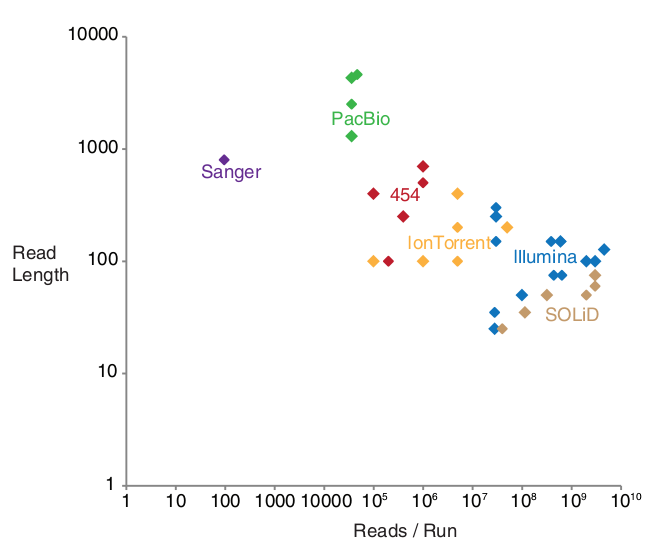
\includegraphics[scale=.55]{figure/read_per_run} 
  
  }
  
  \caption[Présentation de la taille des reads et du nombre de reads par run en fonction de la technologie de séquençage utilisée]{Présentation de la taille des reads et du nombre de reads par run en fonction de la technologie de séquençage utilisée d'après [@Hodkinson2015] : Sequencing space based on read length (in bases) and number of reads per run. Points represent official platform/chemistry combination releases and are color-coded based on the platform family. To see this illustration in color, the reader is referred to the web version of this article at www.liebertpub.com/wound}\label{fig:readPerRun}
  \end{figure}
  
  \subsubsection{La capture des parties à séquencer, avantage et
  inconvenants}\label{la-capture-des-parties-a-sequencer-avantage-et-inconvenants}
  
  Pour de nombreuse application, il peut être intéressant de ne séquencer
  qu'une partie du génome et non pas son intégralité. Dans cette sous
  partie de génome ciblé on peut trouver par exemple : une région
  génomique spécifique à laquelle une pathologie a déjà été associé,
  l'ensembles des exons de certains gènes candidats, ou encore
  l'intégralité des exons de l'ensemble des gènes codant pour une
  protéine. Dans ce dernier cas on parle alors de séquençage exomique ou
  \emph{whole exome sequencing} (WES). Les principaux avantages du WES par
  rapport au WGS sont son cout réduit ainsi qu'une masse de données moins
  importantes à stocker et à analyser. En effet, l'ensemble de l'exome ne
  représente qu'environ 1\% du génome entier. Pour ces raisons, le WES
  considéré comme le standard dans le cadre de recherche sur des
  pathologies génétiques et se révèle être un outil puissant pour
  l'identification de variants associés à des pathologies (S. B. Ng et
  al., \protect\hyperlink{ref-Ng2010}{2010}). Le procédé de séquençage est
  identique au WGS, il est simplement précédé d'une étape d'enrichissement
  au cours de laquelle les exons sont capturés par hybridation à des
  sondes. De fait les exons capturés sont donc dépendant du kit de capture
  utilisé, cette technique permet donc de séquencer uniquement les exons
  connus et ciblés par les sondes. Il faut également noter que depuis
  quelques années, plusieurs études ont remis en cause l'intérêt du WES au
  profit du WGS, notamment car le WGS fournit une meilleure couverture sur
  l'exome que le WES (Lelieveld, Spielmann, Mundlos, Veltman, \& Gilissen,
  \protect\hyperlink{ref-Lelieveld2015}{2015}, Meienberg, Bruggmann,
  Oexle, \& Matyas (\protect\hyperlink{ref-Meienberg2016}{2016})), de plus
  le WES montre une plus grande sensibilité au pourcentage de GC contenu
  dans la région à séquencer et à la sélection des kits de capture
  utilisés (Meienberg et al.,
  \protect\hyperlink{ref-Meienberg2016}{2016}). Ainsi, bien que le WES
  soit encore à l'heure actuelle le choix privilégié dans la majorité des
  études (citation\ldots{}), la réduction des couts de séquençage et de
  stockage des données, il est possible que le WGS remplace totalement le
  WES ainsi que l'ensemble des techniques impliquant la capture de
  séquences ciblées (Meienberg et al.,
  \protect\hyperlink{ref-Meienberg2016}{2016}).
  
  \subsubsection{L'amplification}\label{lamplification}
  
  Dans la plupart des technologies, la phase de séquençage est précédée
  par une étape d'amplification de l'ADN. Cette amplification se fait dans
  la grande majorité des cas sur une surface solide excepté pour la PCR en
  émulsion qui s'effectue en phase aqueuse. Elle permet d'obtenir dans une
  région définie plusieurs milliers de copie du même fragment d'ADN,
  appelés des clones. Cette étape assure que le signal émis lors du
  séquençage pourra être distingué du bruit. Chacun de ces \emph{spots}
  d'amplification appelés aussi centre de réaction, se retrouve donc être
  le représentant d'un unique fragment d'ADN et sera ensuite séquencé
  parallèlement aux autres \emph{spots}. Une plateforme de séquençage
  pouvant gérer plusieurs millions de ces centres de réactions
  simultanément, séquençant ainsi plusieurs millions de molécules d'ADN en
  parallèle, donnant ainsi le nom à ces techniques qualifiées de
  séquençage massif en parallèle. Cette étape d'amplification est
  généralement précédée d'une phase de fragmentation de l'ADN. Cette
  fragmentation peut être physique, enzymatique ou bien chimique. Ce sont
  les résidus d'ADN résultant de cette fragmentation qui seront ensuite
  amplifié. Il existe quatre stratégies utilisées pour le clonage de l'ADN
  dans le cadre du NGS :
  
  \begin{enumerate}
  \def\labelenumi{\arabic{enumi}.}
  \tightlist
  \item
    \textbf{La PCR en émulsion ou emPCR} (\textbf{Figure :
    }\ref{fig:ngsampli} - \textbf{a}) : Le patron d'ADN fragmenté simple
    brin est lié à une séquence adaptatrice complémentaire et est capturé
    par une gouttelette aqueuse appelée micelle contenant une bille
    recouverte d'adaptateur complémentaire à celui fixé sur le fragment
    d'ADN ainsi que tous les composant nécessaire à la réaction de PCR. En
    respectant un ratio nombre de molécule d'ADN / nombre de billes, on va
    fixer un seul fragment d'ADN sur chaque bille. Chacune de ces billes
    seront donc, en fin de réaction, recouverte par plusieurs milliers de
    copies de la même séquence d'ADN.\\
  \item
    \textbf{L'amplification par pont sur face solide} (\textbf{Figure :
    }\ref{fig:ngsampli} - \textbf{b}) : Les fragments d'ADN sont liés à
    des séquences adaptatrices et liée par une de leurs extrémités à une
    amorce fixée sur un support solide. Du fait de la dilution, les
    molécules d'ADN se trouvent éloignées les unes des autres. L'extrémité
    libre du fragment interagit avec les amorces situées à proximité
    formant une structure en pont, d'où le nom de PCR en pont ou
    \emph{bridge-PCR}. La PCR va alors synthétiser un deuxième brin
    complémentaire aux fragments immobilisés sur le support. En procédant
    à des cycles de température comme pour une réaction PCR classique, on
    obtient à l'emplacement de chaque molécule initiale un massif de
    molécules fixées sur la plaque, toutes identiques à la molécule
    initiale.\\
  \item
    \textbf{Amplification par modèle mobile ou \emph{walking-template}
    }(\textbf{Figure : }\ref{fig:ngsampli} - \textbf{c}) : L'ADN fragmenté
    est lié à un adaptateur et lié à une amorce complémentaire fixée sur
    un support solide. Le brin complémentaire du fragment sera synthétisé
    par PCR à partir de l'amorce fixée. La molécule double brin
    nouvellement formée sera ensuite partiellement dénaturée permettant à
    l'extrémité libre de se fixée à une séquence amorce voisine. Des
    amorces \emph{reverse} sont ensuite utilisées pour resynthétiser un
    fragment d'ADN libre à partir des fragments fixés sur le support.\\
  \item
    (\textbf{Figure : }\ref{fig:ngsampli} - \textbf{d}) : \textbf{PAS DU
    TOUT COMPRIS LE MECHANISME !!! }
  \end{enumerate}
  
  \begin{figure}
  
  {\centering 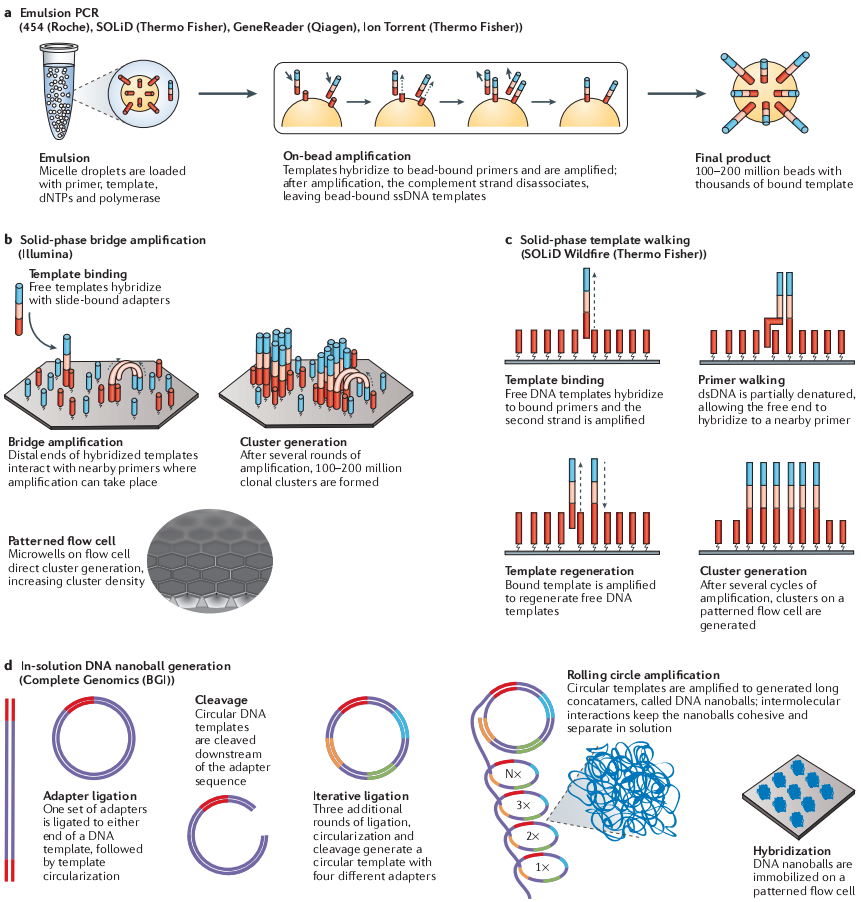
\includegraphics[scale=.455]{figure/ngs_amplification} 
  
  }
  
  \caption[Présentation des différentes stratégies d'amplification de l'ADN dans le cadre du NGS]{Présentation des différentes stratégies d'amplification de l'ADN dans le cadre du NGS d'après [@Goodwin2016] : **a** : PCR en émulsion. **b** : amplification par pont. **c** : Amplification par modèle mobile. **d** : }\label{fig:ngsampli}
  \end{figure}
  
  \subsubsection{La réaction de séquence}\label{la-reaction-de-sequence}
  
  La réaction de séquence est l'étape suivant l'amplification et consiste
  à déterminer l'ordre dans lequel se succèdent les nucléotides de
  l'ensemble des clones générés dans la phase d'amplification. Il existe
  deux technologies principales permettant le séquençage de \emph{reads}
  courts :\\
  
  \begin{enumerate}
  \def\labelenumi{\arabic{enumi}.}
  \tightlist
  \item
    \textbf{Séquençage par synthèse} (SBS) : Ce type de séquençage
    regroupe l'ensemble des méthodes utilisant l'ADN polymérase pour
    synthétiser de l'ADN. En 2016, Sahra Goodwin et ses collègues ont
    différentiés deux catégories de séquençage par synthèse (Goodwin,
    McPherson, \& McCombie, \protect\hyperlink{ref-Goodwin2016}{2016}) :
  
    \begin{enumerate}
    \def\labelenumii{\alph{enumii}.}
    \tightlist
    \item
      \textbf{Terminaison par cycle réversible}, \emph{cyclic reversible
      termination} (CRT) (\textbf{Figure : }\ref{fig:crtSeq}) : Cette
      méthode est caractérisée par son utilisation de molécule dîtes
      terminatrices auxquelles le groupement \(\mathrm{3'-OH}\) est
      modifié de sorte à éviter l'élongation (J. Guo et al.,
      \protect\hyperlink{ref-Guo2008}{2008}), on parlera de groupement
      \(\mathrm{3'-bloqué}\). Le processus est initialisé une amorce est
      liée au fragment d'ADN et permettra l'initialisation de la
      polymerisation. À chaque cycle, un mixe comprenant l'ensemble des
      quatre de desoxynucléotides (dNTPs), préalablement labélisés par un
      fluorophore et \(\mathrm{3'-bloqué}\) sont mis en contact du
      fragment. Après l'incorporation d'un unique dNTP au fragment, les
      dNATP non liés sont éliminée et la nature du dNTP ajouté est
      identifé grace à son fluorophore. Le fluorophore et le groupement
      \(\mathrm{3'-bloqué}\) sont retirés permettant ainsi à un nouveau
      cycle de commencer.
    \end{enumerate}
  \end{enumerate}
  
  \begin{figure}
  
  {\centering 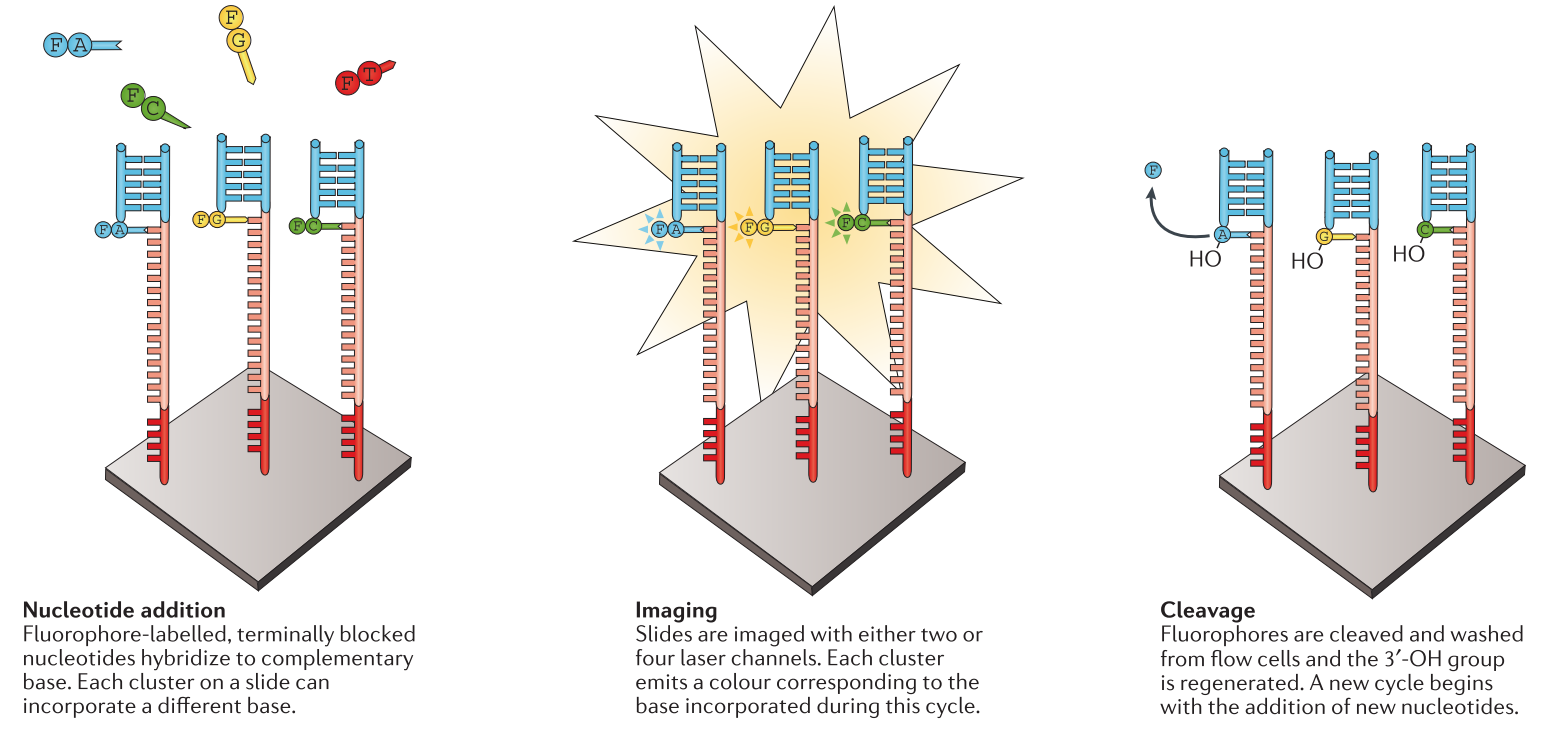
\includegraphics[scale=.28]{figure/CRT_seq_illumina} 
  
  }
  
  \caption[Exemple de séquençage CRT tel qu'il est effectué par Illumina]{Exemple de séquençage CRT tel qu'il est effectué par Illumina d'après [@Goodwin2016] : **a** : ajout d'un dNTP labellisé par un fluorophore et 3'-bloqué. **b** : identification du dNTP ajouté grâce au fluorophore. **c** : le fluorophore est clivé du dNTP et le groupement 3'-OH est reformé à partir du groupement 3'-bloqué permettant ainsi l'élongation}\label{fig:crtSeq}
  \end{figure}
  
  \begin{enumerate}
  \def\labelenumi{\alph{enumi}.}
  \setcounter{enumi}{1}
  \tightlist
  \item
    \textbf{Addition de nucléotide unique}, \emph{single nucleotide
    addition} (SNA) (\textbf{Figure : }\ref{fig:snaSeq}) :
    L'initialisation de la méthode SNA est identique à celle de la méthode
    CRT. La différence se fait donc au moment de la phase d'élongation.
    Contrairement à la méthode CRT, le mixe contenant les dNTPs ne
    contient qu'un seul type de dNTP. Quatre mixes différents sont donc
    présentés successivement au fragment d'ADN à séquencé, ceux-ci se
    fixeront uniquement s'ils sont complémentaires à la séquence. Ces
    dNTPs n'ont donc pas besoin d'être \(\mathrm{3'-bloqué}\) puisqu'un
    seul dNTP est ajouté à chaque itération. Après avoir présenté un mixe,
    vérifie si un dNTP s'est lié au fragment. Lors des séquences
    homopolymériques (plusieurs nucléotides identiques successifs dans la
    séquence), plusieurs dNTP sont donc lié simultanément, cela sera
    détecté car le signal émis sera proportionnel au nombre de nucléotides
    ajoutés.
  \end{enumerate}
  
  \begin{figure}
  
  {\centering 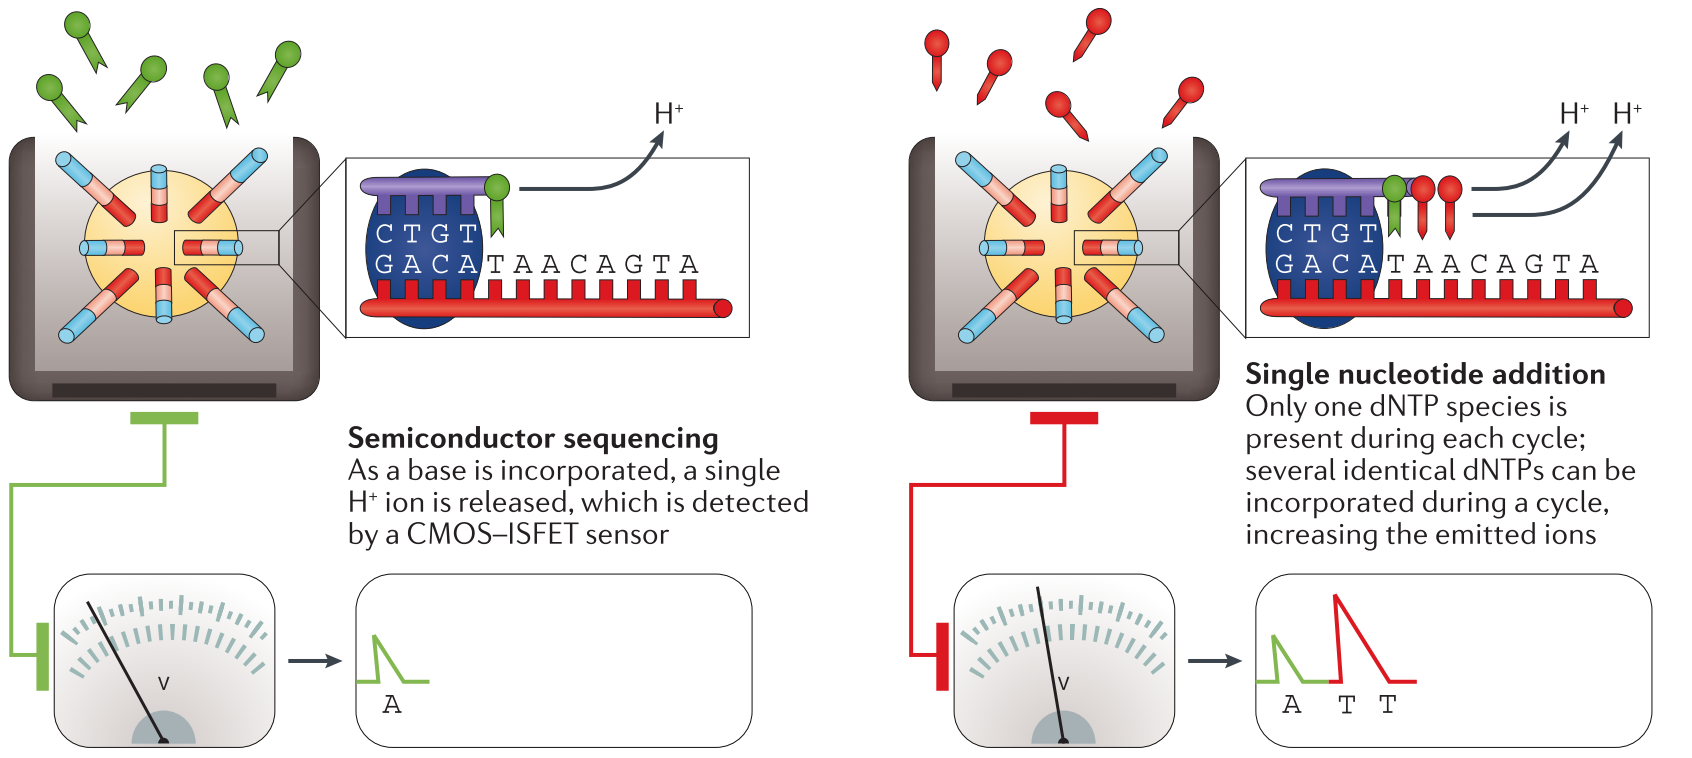
\includegraphics[scale=.26]{figure/SNA_seq_ionTorrent} 
  
  }
  
  \caption[Exemple de séquençage SNA tel qu'il est effectué par Ion Torrent]{Exemple de séquençage SNA tel qu'il est effectué par Ion Torrent d'après [@Goodwin2016] : **a** : Mise en présence du patron d'ADN à séquencer avec un mix contenant un seul type de dNTP, si le dNTP est complémentaire au patron, il se fixe et libère un proton permettant d'identifier la liaison. **b** : Dans d'homopolymère, plusieurs nucléotides identiques successifs, autant de proton sont relâché que de constituant de bases constituant l'homopolymère, le signal émit est donc plus fort permettant d'identifier le nombre des dNTPs liés}\label{fig:snaSeq}
  \end{figure}
  
  \begin{enumerate}
  \def\labelenumi{\arabic{enumi}.}
  \setcounter{enumi}{1}
  \tightlist
  \item
    \textbf{Séquençage par ligation} (SBL) : Par définition, cette méthode
    est basée sur l'hybridation et la ligation de l'ADN (Tomkinson,
    Vijayakumar, Pascal, \& Ellenberger,
    \protect\hyperlink{ref-Tomkinson2006}{2006}) d'une sonde liée à un
    fluorophore. Ce processus utilise les caractéristiques de la ligase,
    une enzyme qui a pour fonction de catalyser la liaison de deux brins
    d'ADN par des liaison phosphodiester. La sonde est constituée d'une ou
    deux bases connues, on parle alors de \emph{one-base-encoded probes}
    ou de \emph{two-bases-encoded probes} suivis d'une succession de bases
    ``dégénérées'' ou universelle, c'est à dire, des bases capables de
    s'apparier avec n'importe laquelle des quatre bases de l'ADN.
  \end{enumerate}
  
  \begin{figure}
  
  {\centering 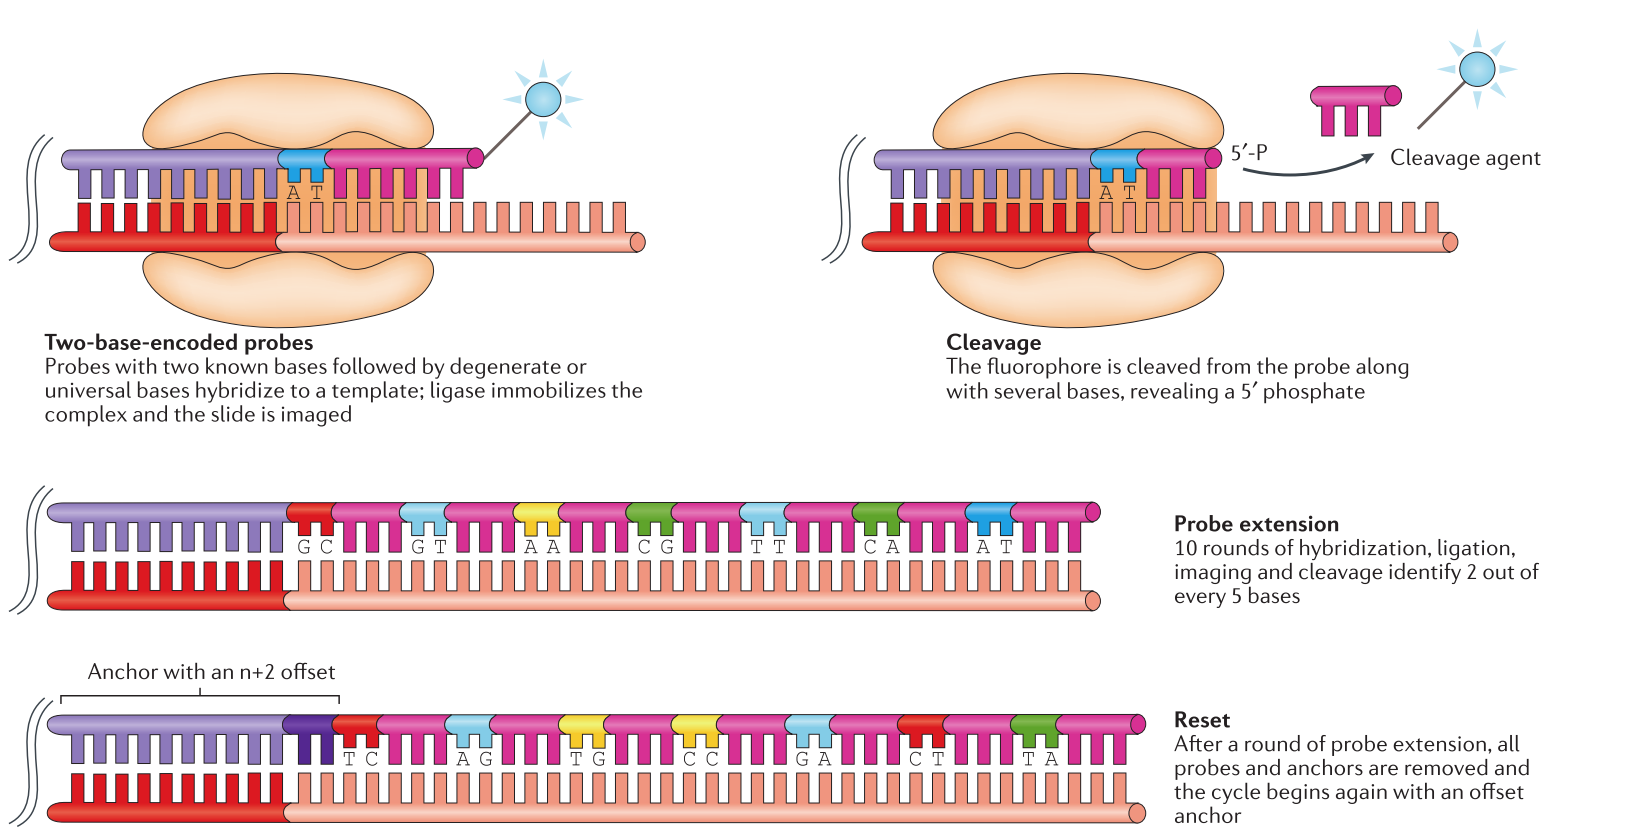
\includegraphics[scale=.26]{figure/SBL_seq_solid} 
  
  }
  
  \caption[Exemple de séquençage SBL tel qu'il est effectué par SOLiD]{Exemple de séquençage SBL tel qu'il est effectué par SOLiD d'après [@Goodwin2016] : }\label{fig:sblSeq}
  \end{figure}
  
  \newpage  
  
  \section{L'analyse bioinformatique des données de
  NGS}\label{lanalyse-bioinformatique-des-donnees-de-ngs}
  
  La stratégie consistant à séquencer en parallèle plusieurs milliers de
  \emph{reads} court a engendré plusieurs nouveaux défis bioinformatique
  dans l'analyse et l'interprétation des données de séquençage et la
  recherche de variants dans le génome humain (Wold \& Myers,
  \protect\hyperlink{ref-Wold2007}{2007}, M. Q. Yang et al.
  (\protect\hyperlink{ref-Yang2009}{2009})). Ces techniques ont été
  appliquées dans différents contextes, notamment la métagénomique (J. Qin
  et al., \protect\hyperlink{ref-Qin2010}{2010}), la détection de SNPs
  (Van Tassell et al., \protect\hyperlink{ref-VanTassell2008}{2008}) et de
  variants structuraux (Alkan et al.,
  \protect\hyperlink{ref-Alkan2010}{2010}, Medvedev, Stanciu, \& Brudno
  (\protect\hyperlink{ref-Medvedev2009}{2009})) mais également dans des
  études portant sur la méthylation de l'ADN (K. H. Taylor et al.,
  \protect\hyperlink{ref-Taylor2007}{2007}), l'analyse de l'expression des
  ARNs messagers (Sultan et al.,
  \protect\hyperlink{ref-Sultan2008}{2008}), dans la génétique du cancer
  (Guffanti et al., \protect\hyperlink{ref-Guffanti2009}{2009}) et la
  médecine personnalisée (Auffray, Chen, \& Hood,
  \protect\hyperlink{ref-Auffray2009}{2009}). Cependant, pour l'ensemble
  de ces applications, la grande quantité de données générées par chaque
  analyse pose plusieurs défis informatiques (Horner et al.,
  \protect\hyperlink{ref-Horner2009}{2009}). En effet, les progrès
  techniques des dernières décennies ont rendu possible le séquençage de
  plusieurs millions des \emph{reads} d'ADN en un temps relativement court
  et à couts raisonnable. Ainsi, l'émergence du séquençage haut débit et
  notamment du WGS et du WES a permis de réunir une quantité jusqu'à
  présent inégalé d'information sur les variations génétiques, et d'une
  manière plus générale, sur les gènes et leurs fonctions (E. R. Mardis,
  \protect\hyperlink{ref-Mardis2008}{2008}, Bentley
  (\protect\hyperlink{ref-Bentley2006}{2006})). Cependant, de par leur
  nature et leur quantité, l'acquisition de ces nouvelles données a
  engendrée de nouvelles problématiques qui freinent les biologistes dans
  leurs recherches.
  
  \subsection{Les données fournies par le
  NGS}\label{les-donnees-fournies-par-le-ngs}
  
  \subsubsection{\texorpdfstring{Un \emph{read} c'est quoi
  ?}{Un read c'est quoi ?}}\label{un-read-cest-quoi}
  
  Après la phase d'amplification, chaque clone est analysé puis, la
  séquence composant chacun de ce clone est déterminée. La taille de cette
  séquence varie en fonction des plateformes de séquençage mais est
  généralement comprise entre 40 et 150 pb pour le NGS (\textbf{Figure :
  }\ref{fig:readPerRun}). Il existe deux types de \emph{reads} :
  
  \begin{enumerate}
  \def\labelenumi{\arabic{enumi}.}
  \tightlist
  \item
    \textbf{\emph{Read single-end} }:\\
  \item
    \textbf{\emph{Read paired-end} }: Avec le séquençage de
    \emph{paired-end reads} les deux extrémités (les \emph{ends}) du
    fragment d'ADN est désormais séquencée. La distance séparant les deux
    extrémités du \emph{read} étant connue, cela permet aux aligneurs
    d'utiliser cette information afin d'améliorer leur précision,
    notamment dans les zones répétées (H. Li et al.,
    \protect\hyperlink{ref-Li2008}{2008}). En plus de SNP, ce format
    permet de mettre en évidence des variants structuraux (Korbel et al.,
    \protect\hyperlink{ref-Korbel2009}{2009}).
  \end{enumerate}
  
  \subsubsection{Le format FASTQ}\label{le-format-fastq}
  
  Le format FASTQ (\textbf{Figure : }\ref{fig:fastqformat}) est le format
  de donnée le plus couramment retourné par les séquenceur haut-débit à
  l'heure actuelle. Sa création est cependant antérieure à l'émergence du
  NGS puisqu'il fut inventé à la fin du XX\(^{ième}\) par Jim Mullikin au
  \href{https://fr.wikipedia.org/wiki/Wellcome_Trust_Sanger_Institute}{Wellcome
  Trust Sanger Institute} alors que le séquençage commencait à prendre de
  l'ampleur grâce à des projets tel que le
  \href{https://fr.wikipedia.org/wiki/Projet_G\%C3\%A9nome_Humain}{Projet
  Génome Humain}. La quantité de donné générées par ces programmes à
  nécessité une analyse automatisé, c'est ainsi que chaque base séquencée
  s'est vue associé un score de qualité appelé \emph{Phred-score}. Chaque
  séquence générait ainsi deux fichiers, un fichier FASTA contenant les
  séquences et un fichier QUAL contenant les scores \emph{Phred} associés
  à chaque base du fichier FASTA Cock2009. Plus tard, afin de n'avoir à
  manipuler qu'un seul fichier, les fichiers FASTA et QUAL furent
  fusionnés en ce que l'on appelle désormais le fichier FASTQ. Ce format
  est aujourd'hui le plus utilisé par les différents séquenceurs on peut
  noter certaines différences dans les formats FASTQ provenant des
  différentes plateformes puisqu'à l'époque, aucune spécification
  officielle n'avait été donnée (Cock, Fields, Goto, Heuer, \& Rice,
  \protect\hyperlink{ref-Cock2009}{2009}).
  
  \begin{figure}
  
  {\centering 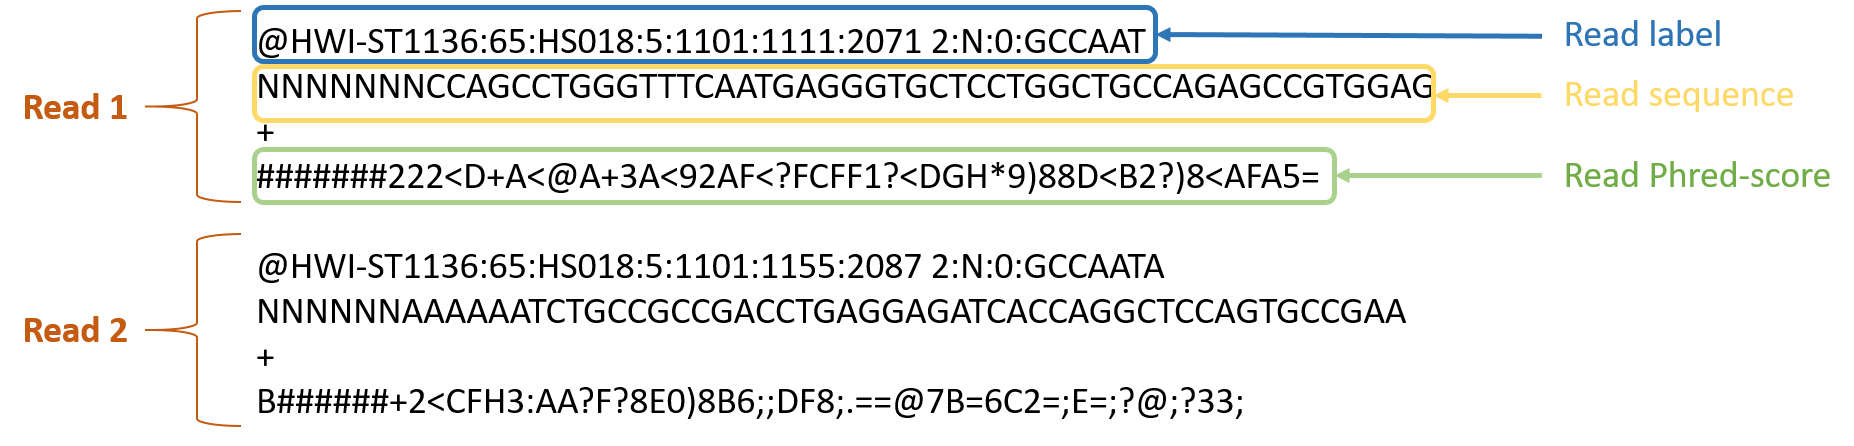
\includegraphics[scale=.55]{figure/fastq} 
  
  }
  
  \caption[présentation d'un fichier FASTQ (FIGURE A CHANGER)]{présentation d'un fichier FASTQ (FIGURE A CHANGER) : **a** : identifiant du *read*. **b** : séquence du *read*. **c** : score de qualité associé}\label{fig:fastqformat}
  \end{figure}
  
  \hypertarget{lalignement}{\subsection{L'alignement}\label{lalignement}}
  
  L'alignement constitue la première étape de l'analyse des données de NGS
  lorsqu'un génome de référence est disponible. L'objectif de l'alignement
  est de déterminer la position correcte de chacun des \emph{reads}
  séquencés le long du génome de référence. Cette référence est souvent
  construite à partir des données de séquençage de plusieurs donneurs et
  ne représente donc pas la séquence d'un individu en particulier mais est
  censé représenter la séquence consensus d'une espèce donnée. Par
  exemple, la séquence de référence humaine GRCh37 (\emph{Genome Reference
  Consortium human build 37}) a été créés à partir de 13 volontaires
  anonymes New-Yorkais. Dès lors, cette référence servira de patron aux
  aligneurs afin qu'ils replacent correctement les différents \emph{reads}
  des individus séquencés. Cette étape peut être comparée à la
  reconstruction d'un puzzle dans laquelle les \emph{reads} seraient les
  pièces et le génome de référence le modèle. Elle constitue probablement
  l'étape la plus importante de l'analyse des données issues du séquençage
  haut débit (Flicek \& Birney, \protect\hyperlink{ref-Flicek2009}{2009})
  car elle est la base sur laquelle reposent l'ensemble des étapes
  effectuées en aval, notamment l'appel des variants (R. Nielsen, Paul,
  Albrechtsen, \& Song, \protect\hyperlink{ref-Nielsen2011}{2011}).
  Cependant, l'étape d'alignement peut est sujette à de nombreuses erreurs
  dont certaines proviennent directement des erreurs de survenues lors de
  l'étape de séquençage, d'autres, sont dues aux caractéristiques des
  régions séquencées comme par exemple les séquence répétées (Ben Langmead
  \& Salzberg, \protect\hyperlink{ref-Langmead2012}{2012}) qui pourront
  entrainer l'alignement d'un même \emph{read} à plusieurs régions du
  génome (Treangen \& Salzberg,
  \protect\hyperlink{ref-Treangen2013}{2013}). De nombreux aligneurs ont
  émergé afin de répondre au mieux à cette problématique tel que Bowtie (B
  Langmead, Trapnell, Pop, \& Salzberg,
  \protect\hyperlink{ref-Langmead2009}{2009}), Bowtie2 (Ben Langmead \&
  Salzberg, \protect\hyperlink{ref-Langmead2012}{2012}), BWA, NovoAlign,
  MAGIC (Su et al., \protect\hyperlink{ref-Su2014}{2014}). De nombreuse
  études ont cependant montrées de grandes différences entre ces
  aligneurs, au niveau du temps de calcul, de leur cout en mémoire et de
  leur taux d'erreur (Ruffalo, Laframboise, \& Koyutürk,
  \protect\hyperlink{ref-Ruffalo2011}{2011}, Thankaswamy-Kosalai, Sen, \&
  Nookaew (\protect\hyperlink{ref-Thankaswamy-Kosalai2017}{2017}), S. Bao
  et al. (\protect\hyperlink{ref-Bao2011}{2011})).
  
  \subsection{L'appel des variants}\label{lappel-des-variants}
  
  L'appel des variants, ou \emph{variant calling}, fait référence à
  l'ensemble des méthodes permettant d'identifier des SNVs ou des indels à
  partir des résultats de l'alignement. Cette étape est souvent
  différenciée de l'alignement, cependant, les résultats de l'appel étant
  extrêmement dépendant de l'alignement, il est conseillé d'effectuer son
  appel en tenant compte de l'aligneur choisi (R. Nielsen et al.,
  \protect\hyperlink{ref-Nielsen2011}{2011}, M. A. DePristo et al.
  (\protect\hyperlink{ref-DePristo2011}{2011}), Lunter \& Goodson
  (\protect\hyperlink{ref-Lunter2011}{2011})). On appellera variants
  toutes différences de séquence observées entre un individu et la
  séquence de référence utilisée. Pour reprendre la comparaison avec la
  construction d'un puzzle, cette étape consiste à détecter quels sont les
  pièces qui présentent des différences avec le modèle. De nombreux
  logiciels d'appel des variants, ou \emph{caller}, basés sur des
  algorithmes différents ont émergés ces dernières années pour répondre à
  cette problématique. Parmi les plus connus on note SAMtools (H. Li et
  al., \protect\hyperlink{ref-Li2009}{2009}), Genome Analysis Tool Kit -
  HaplotypeCaller (GATK-HC) (McKenna et al.,
  \protect\hyperlink{ref-McKenna2010}{2010}), Freebayes, SOAPindel et TVC.
  Les quatre premiers cités, peuvent être utilisés pour analyser des
  données provenant de tout type de plateforme de séquençage contrairement
  à TVC qui a été développé spécifiquement pour les données provenant de
  Ion Proton. Les données issues de NGS peuvent présenter un taux d'erreur
  important. Ce taux d'erreur est multifactoriel et inclus notamment les
  erreurs de l'alignement. L'un des éléments clef à prendre en compte pour
  pouvoir effectuer un appel de qualité est la couverture de la position
  appelée (D. Sims et al., \protect\hyperlink{ref-Sims2014}{2014}).
  Cependant, malgré la prise en compte de cet élément, l'appel de variants
  reste un processus difficile souvent lié à plusieurs erreurs. Plusieurs
  de ces erreurs sont même directement liées à la plateforme de séquençage
  utilisée en amont, et les différents logiciels ne présentent pas les
  mêmes performances en fonction de ces différentes plateforme (Hwang,
  Kim, Lee, \& Marcotte, \protect\hyperlink{ref-Hwang2015}{2015}), c'est
  pourquoi il convient d'adapter le logiciel d'appel en fonction de la
  plateforme de séquençage utilisée préalablement. Les erreurs d'appel
  sont généralement classées en deux catégories principales et certains
  aligneurs auront tendance à être plus sujets à l'un de ces types
  d'erreur qu'à l'autre (\textbf{Figure : }\ref{fig:snperror}) :
  
  \begin{enumerate}
  \def\labelenumi{\arabic{enumi}.}
  \tightlist
  \item
    Oubli de l'allèle de référence (\textbf{IR}, \emph{ignore the
    reference allele}) : représente un variant appelé homozygote
    correspondant en réalité à un variant hétérozygote composé de l'allèle
    de référence et d'un allèle variant.\\
  \item
    Ajout de l'allèle de référence (\textbf{AR}, \emph{adding the
    reference allele}) : représente un variant appelé hétérozygote composé
    de l'allèle de référence et d'un allèle variant correspondant en
    réalité à un variant homozygote composé de deux allèles variants.\\
  \end{enumerate}
  
  \begin{figure}
  
  {\centering 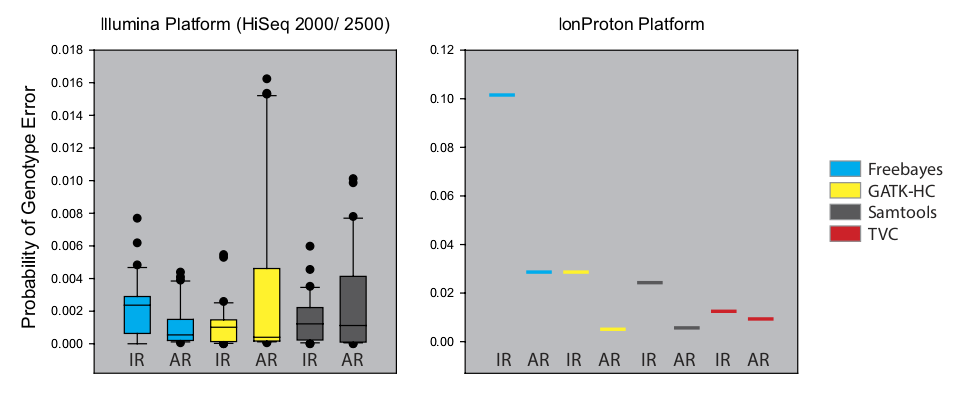
\includegraphics[scale=.50]{figure/snp_error_type} 
  
  }
  
  \caption[Représentation des erreurs d'appel de type IR et AR en fonction de la plateforme de séquençage et du logiciel d'appel]{Représentation des erreurs d'appel de type IR et AR en fonction de la plateforme de séquençage et du logiciel d'appel d'après [@Hwang2015] : Pour la plateforme Illumina, on peut voir que Freebayes préfère les appels variant-homozygote tandis que GATK-HC et Samtools préfèrent les appels hétérozygotes. Pour la plateforme Ion Proton, les 4 logiciels ont une préférence pour les erreurs de type IR}\label{fig:snperror}
  \end{figure}
  
  De même que pour l'aligneur, le choix du logiciel d'appel est crucial
  car il existe de nombreuses différences dans les variants appelés par
  différents logiciels se basant sur les mêmes données brutes (Baes et
  al., \protect\hyperlink{ref-Baes2014}{2014}, O'Rawe et al.
  (\protect\hyperlink{ref-ORawe2013}{2013}), Rosenfeld, Mason, Smith,
  Wallin, \& Diekhans (\protect\hyperlink{ref-Rosenfeld2012}{2012})). En
  effet, en 2013, une étude comparant les résultats de 5 caller montrait
  que seulement 57,4\% des variants étaient appelés par les 5 caller et
  que 80,7\% des variants étaient appelés par au moins 3 d'entre eux. Ce
  taux chutait drastiquement pour les indels puisque la concordance était
  cette fois seulement de 26,8\% pour les indels non retrouvés par les 3
  \emph{caller} (O'Rawe et al., \protect\hyperlink{ref-ORawe2013}{2013}).
  Ces résultats sont cependant à pondérés avec une étude de 2015 comparant
  4 \emph{caller} et montrant que 91,7\% des SNVs séquencés sur une
  plateforme Illumina étaient appelés par 3 \emph{caller}, cependant, pour
  les variants séquencés sur Ion Proton, seulement 27,3\% des variants
  étaient appelés par au moins 3 \emph{caller} et 57,4\% des variants
  n'étaient appelés que par un seul des \emph{caller} (Hwang et al.,
  \protect\hyperlink{ref-Hwang2015}{2015}).
  
  \subsection{L'annotation des variants, filtrage et
  priorisation}\label{lannotation-des-variants-filtrage-et-priorisation}
  
  Traditionnellement, les scientifiques développaient leur expertise dans
  un nombre de pathologie et de gènes associés limité. L'émergence du NGS
  a totalement remis en cause cette pratique, dès lors qu'il est désormais
  courant de retrouver entre 20.000 et 25.000 variants différents par
  exome (Gonzaga-Jauregui, Lupski, \& Gibbs,
  \protect\hyperlink{ref-Gonzaga-Jauregui2012}{2012}). Afin de pouvoir
  lier un variant à une pathologie, il est désormais indispensable
  d'annoter cet ensemble de variant, c'est à dire d'associer à ces
  variants l'ensembles des informations qui les caractérisent afin de
  pouvoir les replacer dans leur contexte biologique. Ces informations
  serviront ensuite d'indicateur afin filtrer ou prioriser un variant.
  Cette dernière étape de l'analyse est elle aussi cruciale puisqu'elle
  permet de réduire le nombre de variant à considérer \ldots{}. On peut
  généralement distinguer deux niveaux d'annotation d'un variant :
  
  \begin{enumerate}
  \def\labelenumi{\arabic{enumi}.}
  \tightlist
  \item
    \textbf{Au niveau du variant} : Ce niveau d'annotation regroupe
    l'ensemble des informations \textbf{spécifiques} à un variant
  
    \begin{enumerate}
    \def\labelenumii{\alph{enumii}.}
    \tightlist
    \item
      \textbf{Informations issues des résultats du séquençage} : la
      couverture du variant ainsi que la qualité qui lui est associée
      peuvent permettre de considérer un variant comme étant. Le génotype
      associé à ce variant est également une information importante.\\
    \item
      \textbf{La fréquence du variant dans la population générale} :
      l'émergence du séquençage haut-débit a permis de de gros consortium
      tel que ESP6500 {[}CITATION{]}, 1KG {[}CITATION{]}. Ces consortiums
      on put mettre à disposition du public de données de séquençage
      exomique de 6503 individus pour ESP et de 2504 pour la phase 3 du
      1000Genomes. On peut également noter l'\emph{Exome Aggregate
      Consortium} (ExAC) (Lek et al.,
      \protect\hyperlink{ref-Lek2016}{2016}) qui n'a effectuer aucun
      séquençage mais qui à récupérer les données de plusieurs gros jeux
      (notamment 1000Genome et ESP) afin de leur appliquer la même analyse
      bioinformatique harmonisant ainsi les données provenant de 60.706
      individus non apparentés. Cette masse d'information permet de se
      faire une idée de la fréquence d'un variant dans la population
      générale et même au sein de sous population humaine.\\
    \item
      \textbf{Son impact sur le transcrit} : Dans la plupart des analyses
      phénotype-génotype, les chercheurs se limitent au variant
      chevauchant des transcrits codant pour une protéine. Il est donc
      important de savoir l'impact d'un variant sur ce transcrit, c'est à
      dire si le variant va causer une mutation synonyme, un
      faux-sens\ldots{} Des logiciels tel que \emph{Variant Effect
      Predictor} (VEP) (W. McLaren et al.,
      \protect\hyperlink{ref-McLaren2016}{2016}), SnpEff (Cingolani et
      al., \protect\hyperlink{ref-Cingolani2012}{2012}) ou encore ANNOVAR
      {[}@{]} vont prédire l'impact qu'aura un variant sur les différents
      transcrits qu'il chevauche. D'autre logiciel tel que SIFT (P. Kumar,
      Henikoff, \& Ng, \protect\hyperlink{ref-Kumar2009}{2009}), PROVEAN
      (Y. Choi, Sims, Murphy, Miller, \& Chan,
      \protect\hyperlink{ref-Choi2012}{2012}), Polyphen2, ou encore CADD
      vont chercher à prédire la pathogénicité de ce variant, c'est à dire
      la probabilité que ce variant soit délétère pour l'individu qui le
      porte. Bien que cette information soit important, elle est à
      pondérer étant donné le peu de concordance qu'il existe entre les
      prédictions de ces différents logiciel (\textbf{Figure :}
      \ref{fig:vennpred}).
    \end{enumerate}
  \end{enumerate}
  
  \begin{figure}
  
  {\centering 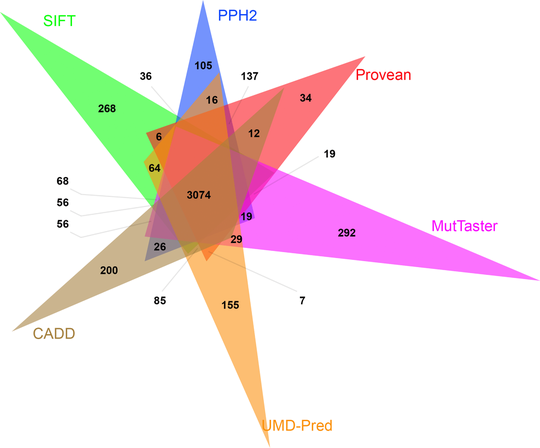
\includegraphics[scale=.7]{figure/venn_Diag_patho_pred} 
  
  }
  
  \caption[Diagramme de Venn des prédictions de pathogénicités de six logiciels]{Diagramme de Venn des prédictions de pathogénicités de six logiciels d'après [@Salgado2016] : }\label{fig:vennpred}
  \end{figure}
  
  \begin{enumerate}
  \def\labelenumi{\arabic{enumi}.}
  \setcounter{enumi}{1}
  \tightlist
  \item
    \textbf{Au niveau de l'unité génétique} : DÉCRIRE UNITÉ GÉNÉTIQUE
    (gène, transcrit). L'annotation au niveau de l'unité génétique
    consiste à récupérer l'ensemble des informations disponible non plus
    sur le variant uniquement mais sur la ou les unités génétiques qu'il
    impacte. Ce ``dézoom'' permet d'ajouter des informations
    complémentaires particulièrement utile notamment lorsque peut
    d'information sont disponibles sur le variant lui-même. En pratique,
    la plupart des variants connues pour impliquer une pathologie sont des
    variants privés, c'est à dire spécifique à une famille ou un individu
    limitant ainsi la quantité d'information disponible sur ce variant.
    Élargir l'annotation au niveau des unités génétiques impactés par des
    variants permet d'augmenter considérablement la quantité d'information
    disponible et permet donc d'améliorer la capacité des algorithmes à
    filtrer et / ou prioriser les variants rendant donc les analyses plus
    efficaces. On peut relever certains logiciels tel que le \emph{Protein
    ANalysis THrough Evolutionary Relationships} (PANTHER) (Mi et al.,
    \protect\hyperlink{ref-Mi2017}{2017}) permet par exemple de classer
    une liste de gènes en fonction de leurs fonctions moléculaires, des
    processus biologiques et des voies de signalisation dans lesquels ils
    sont impliqués. On peut également noter \emph{the Human Phenotype
    Ontology project} (HPO) (Köhler et al.,
    \protect\hyperlink{ref-Kohler2014}{2014}) qui fournit une
    classification (À compléter). Plus récemment, on a pu voir émerger des
    ``scores mutationnel'' tel que RVIS (Petrovski et al.,
    \protect\hyperlink{ref-Petrovski2013}{2013}) ou encore le pLI (Lek et
    al., \protect\hyperlink{ref-Lek2016}{2016}). En se basant sur les
    bases de données telle que ESP ou encore ExAC, ces scores permettent
    de classer les gènes en fonction de leur tolérance (ou intolérance)
    aux variations avec l'idée sous-jacente que ``les gènes impliqués dans
    des pathologies à transmission Mendéliennes'' devraient être moins
    tolérant aux variations que les autres.
  \end{enumerate}
  
  Comme nous l'avons vu, l'accumulation de cette information est
  extrêmement importante puisqu'elle permet aux biologistes de faire face
  à la masse de données générés par le NGS l'aidant ainsi dans ses prises
  de décisions. Il est à noter que la plupart de ces informations sont
  extrêmes dépendantes du jeu de gènes utilisés, les prédictions seront
  donc différentes si l'on se base les gènes RefSeq, Ensembl ou UCSC (D.
  J. McCarthy et al., \protect\hyperlink{ref-McCarthy2014}{2014},S. Zhao
  \& Zhang (\protect\hyperlink{ref-Zhao2015}{2015})) bien que les gènes du
  \emph{Consensus Coding Sequence project} (CCDS) soient bien représentés
  par ces trois listes (K. D. Pruitt et al.,
  \protect\hyperlink{ref-Pruitt2009}{2009}). De même, pour une même liste
  de gêne, de nombreuses différences seront observées en fonction du ou
  des logiciels de prédiction utilisés (D. J. McCarthy et al.,
  \protect\hyperlink{ref-McCarthy2014}{2014}, Salgado, Bellgard,
  Desvignes, \& B??roud (\protect\hyperlink{ref-Salgado2016}{2016})).
  
  \subsection{Conclusion NGS}\label{conclusion-ngs}
  
  En moins de 10 ans, les technologies NGS sont passées du séquençage de
  panel de gènes (environs 100 Mb pour le Roche GS FLX system) au
  séquençage de génome entiers (environs 1500 GB pour l'Illumina Hiseq
  4000) et d'une utilisation exclusive à la recherche à la routine
  clinique. Le nombre croissant de d'études utilisant le WGS ou le WES
  démontre le pouvoir de ces approches dans des analyses
  phénotypes-génotypes impliquant des pathologies à transmission
  Mendelienne. De plus, la diminution constante des couts par génome /
  éxomes séquencés laisse supposer que ces technologies deviendront d'ici
  peut le fer de lance de la génétique clinique moderne. Cependant, cette
  quantité de donnée produites crées de nouvelles problématiques pour les
  généticiens qui se retrouvent désormais face au ``déluge de données
  génétiques'' (Schatz \& Langmead,
  \protect\hyperlink{ref-Schatz2013}{2013}). Le succès d'une étude n'étant
  plus lié aux capacités de séquençage mais aux compétences dans l'analyse
  et l'interprétation des données produites. Bien que de nombreux efforts
  soient pour palier la contrainte instaurée par les \emph{reads} courts
  dans le cadre d'analyse génomique, les solutions informatique et
  bioinformatique proposée jusqu'à présent restent en dessous des besoins
  créés par NGS (J. D. McPherson,
  \protect\hyperlink{ref-McPherson2009}{2009}). Cette masse de données
  produite, à l'origine du succès du séquençage haut-débit dans le domaine
  de la génomique et de la post-génomique, se retrouve désormais être un
  frein dans la compréhension et l'interprétation des réseaux de gènes et
  leurs implications dans des pathologies, la limitation de cette
  technologie n'étant plus le séquençage d'un, de plusieurs, ou de
  l'ensemble des gènes, mais plutôt l'analyse et l'interprétation des
  donnée générée. Le processus allant de l'extraction de l'ADN à
  l'identification d'un variant responsable d'une pathologie comprend de
  nombreuses étapes apportant avec elles leur lot d'erreurs. Bien que dans
  chacune de ces phases, de nombreux acteurs soient en concurrence et
  cherchent à atteindre une solution idéale, celle-ci n'a toujours pas été
  trouvé et la prolifération des logiciels et autres algorithmes
  d'analyses, bien que nécessaire, s'ajoute à la confusion.
  
  Malgré les dizaines de milliers d'exomes et de génomes ayant été jusqu'à
  présent étudiés, notre compréhension des mécanismes moléculaire qui
  sous-tendent la variété génomique humaine reste limité, et ce
  particulièrement dans le contexte de l'analyse de pathologies
  génétiques. En effet, à l'heure actuelle, plus de 3700 pathologie à
  transmission Mendélienne ont été caractérisée mais un nombre similaire
  ont toujours une cause inconnue (Amberger, Bocchini, \& Hamosh,
  \protect\hyperlink{ref-Amberger2011}{2011}).L'élucidation de ces
  mystères passera probablement par une harmonisation de méthodes de
  production des données ainsi que par l'amélioration des techniques
  d'analyses.
  
  \hypertarget{globo}{\chapter{Investigation génétique et physiologique de
  la globozoospermie}\label{globo}}
  
  \chapter{MutaScript}\label{mutascript}
  
  \section{Introduction}\label{introduction}
  
  Il y a quelques années, le séquençage Sanger était encore massivement
  utilisé en recherche clinique. Cette technique étaiy extremement
  couteuse en temps et en argent freinant considérablement la progression
  des recherches du type phénotype-génotype de sorte qu'en 2011, les
  causes de plus de 3.500 pathologies à transmission Mendelienne restaient
  inconnus (Stitziel, Kiezun, \& Sunyaev,
  \protect\hyperlink{ref-Stitziel2011}{2011}). L'emmergence du séquençage
  haut-débit a immédiatement initié une nouvelle ère dans le domaine de la
  recherche clinique et permettant dans un temps record et à cout
  raisonnable d'obtenir la séquence de l'intégralité du génome ou bien des
  régions exomiques. Ce bond technologique est à l'originbe de grandes
  avancées permettant de lier plus de \ldots{} variants génétiques à une
  pathologie mendelienne {[}citation{]}.\\
  Cependant, de part sa masse, les données produites crées de nouvelles
  problématiques pour les généticiens qui se retrouvent désormais face au
  ``déluge de données génétiques'' (Schatz \& Langmead,
  \protect\hyperlink{ref-Schatz2013}{2013}). En effet, un génome humain
  typique compte en moyenne 3,5 millions de variants différents et plus de
  1000 variations du nombre de copies (CNVs) (Gonzaga-Jauregui et al.,
  \protect\hyperlink{ref-Gonzaga-Jauregui2012}{2012}) après comparaison
  avec le génome de référence. Parmis ceux-ci, 20.000-25.000 d'entre eux
  impactent des régions codant pour une protéine avec environs 10.000
  variants impliquant un changement d'acide aminé et 50-100 prédit comme
  tronquant la protéine (Gonzaga-Jauregui et al.,
  \protect\hyperlink{ref-Gonzaga-Jauregui2012}{2012}). Ainsi, les analyses
  fastidieuse permettant de mettre en évidence le variant responsable de
  la pathologie font desormais partit du quotidien des généticiens.
  Appliquer ces tache est d'autant plus laborieux qu'elles nécéssites
  entre autres des compétences en informatique et en statistiques qui sont
  assez éloignées des compétences ``traditionelles'' des généticiens. De
  manière générale, ces analyses se découpent en trois étapes principales.
  La première est l'étape d'alignement qui basiquement consiste à aligner
  les \emph{reads} générés lors de l'étape de séquençage le long d'un
  génome de référence. Une fois cela fait, l'étape d'appel des variants
  consiste à recensser l'ensembles des ``différences'' observées entre les
  données de l'individu séquencé et le génome de référence permettant
  ainsi d'établire une liste de SNVs et de petites insertions / délétions
  (indels) avec leur génotype associés. Comme dit précédement, cette liste
  peut atteindre 25.000 variants différents par individus. La dernière des
  étapes regroupe l'annotation et le filtrage des variants. Elle
  représente souvent la faiblesse des analyses phénotype-génotype puisque
  dans une grande partie des cas, le pouvoir filtrant n'est pas assez
  puissant pour obtenir une liste de variants suffisamant petite pour
  qu'elle soit interprétable par l'homme, ainsi le variant causal se
  retrouve bien souvent noyé parmi d'autre variant rendant l'analyse et
  l'interprétation moins efficaces.\\
  Améliorer la qualité de l'annotation et le filtrage des variants dans
  les analyses phénotype-génotype se révèle donc être une des clés
  permettant d'améliorer l'efficience de ces analyses, c'est pourquoi nous
  avons déveloper le score MutaScript. Ce score a pour but de classer
  l'ensemble des transcrit codant en fonction de leur charge mutationelle
  avec l'idée sous-jacente que les transcrits les plus mutés dans la
  population générale ne sont porbablement pas impliqués dans des
  pathologies sévères à transmission Mendelienne et, \emph{a contrario}
  ceux retrouvés comme n'étant pas / peu mutés le sont probablement. Pour
  ce faire, le score MutaScript repose sur trois (\ldots{}). La première
  étant le jeux de transcrit fournit par Ensembl (B. L. Aken et al.,
  \protect\hyperlink{ref-Aken2017}{2017}) qui comporte \ldots{} transcrits
  codants. Afin de connaitre la harge mutationelle des ces transcrits,
  nous nous sommes basées sur les variants mis à disposition par \emph{the
  Exome Aggragate Consortium} (ExAC) (Lek et al.,
  \protect\hyperlink{ref-Lek2016}{2016}) qui réunit les données d'exome de
  60.706 individus non apparentés que nous avons ensuite annoté grâce au
  logiciel \emph{variant effect predictor} (VEP) (W. McLaren et al.,
  \protect\hyperlink{ref-McLaren2016}{2016}) afin de prédire l'impacte de
  chaque variant sur l'ensemble des transcrits qu'ils chevauchent de sorte
  à ce que les variants ayant un impacte prédit commé étant délétère aient
  une plus grosse contribution au score MutaScript que ceux ayant un
  impacte faible. À l'heure actuelle, plusieurs logiciels tel que SIFT (P.
  Kumar et al., \protect\hyperlink{ref-Kumar2009}{2009}) ou encore
  PolyPhen-2 (I. A. Adzhubei et al.,
  \protect\hyperlink{ref-Adzhubei2010}{2010}). Cependant, ces logiciels
  donnent un score pour un variant et n'extrapolent pas leurs prédictions
  aux niveau du gènes et/ou du transcrits. D'autres logiciels tel que
  Exomiser (Robinson et al., \protect\hyperlink{ref-Robinson2014}{2014})
  et Endeavour (Tranchevent et al.,
  \protect\hyperlink{ref-Tranchevent2016}{2016}) cependant, pour pouvoir
  fonctionner, ces logiciels nécéssitent d'avoir des connaissances
  génétiques sur la pathologie étudiée. Plus récemment, favorisé par
  l'emmergence de gros jeux de données exomiques comme ExAC, d'autres
  scores ont vu le jour tel que le \emph{residual variance intoler- ance
  score} (RVIS) (Petrovski et al.,
  \protect\hyperlink{ref-Petrovski2013}{2013}) ou encore \emph{the the
  Probability of loss-of-function Incoherency} (pLI) (Lek et al.,
  \protect\hyperlink{ref-Lek2016}{2016}). MutaScript se présente comme une
  alternative à ces derniers scores et, bien que sa fonction soit
  similaire, il diffère de ceux-ci sur de nombreux points. Tout d'abord,
  MutaScript donne un score à l'ensemble des transcrits codant pour une
  protéine là où pLI donne un score seulement au transcrit consensus de
  chaque gène et RVIS qui aggrege les séquence codante de l'ensemble des
  transcrits d'un même gène créant ainsi un transcrit ``chimérique''. Ce
  procédé, bien qu'il facilite l'interprétation du score, engendre une
  perte d'information puisque l'on se retrouve avec un seul score par gène
  et non par transcrits. De plus, dans la conception de leur score, RVIS
  et pLI ne consifère que les variants dit \emph{loss-of-function} (LoF),
  c'est à dire les variants impactant l'epissage, engendrant un codont
  strop ou un décallage du cadre de lecture. Cependant, ces variants ne
  représentent que \ldots{}\% des variants fournit par la base de données
  ExAC. C'est pourquoi, MutaScript prend en compte l'ensemble des
  variants, peut importe leur impacte sur les différents transcrits qu'ils
  chevauchent, et leur attribue un poid en fonction de cet impacte de
  sorte à ce que les variants délétères contribuent plus au score d'un
  transcrits que les autres. Aussi, l'étude des scores RVIS et pLI nous a
  permis de mettre en évidence une corrélation forte entre le score qu'ils
  attribuent à un gène et la taille de la séquence codante (CDS) de ce
  même gène. Cette corrélation étant principalement due à un biais causé
  par leur manière de calculer leur score et non à une réalité biologique,
  MutaScript fut construit de sorte à éviter cette corrélation qui peut
  mener à des erreurs d'interprétations. Afin d'évaluer le score
  MutaScript nous l'avons confrontés au RVIS (Petrovski et al.,
  \protect\hyperlink{ref-Petrovski2013}{2013}) ainsi qu'à pLI (Lek et al.,
  \protect\hyperlink{ref-Lek2016}{2016}) afin de comparer à la fois leur
  capacité à prédire les gènes intolérant aux variation en se basant sur
  des listes de gènes fournit par \emph{the human phenotype ontology}
  (HPO) (Köhler et al., \protect\hyperlink{ref-Kohler2014}{2014}) mais
  aussi en testant sa capaciter à prédire les gènes considérés comme
  ``dispensables'' pour la vie et la reproduction humaine en se basant
  sur\ldots{}
  
  \section{Matériel \& Méthodes}\label{materiel-methodes}
  
  \subsection{Récupération et filtrage des
  données}\label{recuperation-et-filtrage-des-donnees}
  
  \begin{enumerate}
  \def\labelenumi{\arabic{enumi}.}
  \tightlist
  \item
    \textbf{Le jeu de transcrits Ensembl} : Pour cette étude, nous nous
    sommes basés sur la version 75 du jeu de transcrits fournit par
    Ensembl (B. L. Aken et al., \protect\hyperlink{ref-Aken2017}{2017}).
    le fichier gtf contenant les données est téléchargeable
    \href{insérer\%20liens\%20vers\%20gtf}{ici}. Cette version bien
    qu'elle ne soit pas la dernière publiée par Ensembl, est la dernière à
    se basée sur la version GRCH37/hg19 qui est la version du génome qu'a
    choisi ExAC pour effectuer l'alignement de ses données. À partir du
    fichier gtf, seul les transcrit taggés comme codant pour une protéine
    furent conservés, de même, l'ensemble des transcrits ayant une
    couverture mediane \textless{}15 sur plus de 30\% de leur séquence
    codante dans les données ExAC furent filtrés.\\
  \item
    \textbf{Filtrage des variants} :
  
    \begin{enumerate}
    \def\labelenumii{\alph{enumii}.}
    \tightlist
    \item
      Lien pour télécharger le vcf ExAC\\
    \item
      L'ensemble des variants n'ayant pas la mention ``PASS'' dans la
      colonne FILTER du fichier VCF fournit par ExAC furent filtrés.\\
    \item
      L'ensemble des variant n'ayant pas une couverture médiane \(\ge\) 15
      furent filtrés\\
    \item
      L'ensemble des variants intronique (sauf ceux proches des sites
      d'epissage) et les variants situés dans les régions \emph{upstream}
      et \emph{downstream} furent filtrés\\
    \end{enumerate}
  \item
    \textbf{Réannotation des données ExAC} : Afin d'utiliser une version
    plus récente de VEP, l'annotation fut effectuées avec le logiciel VEP
    version 81 en utilisant la version 75 des transcrits Ensembl (INSÉRER
    LA COMMANDE)
  \end{enumerate}
  
  \subsection{Validation du score}\label{validation-du-score}
  
  \begin{enumerate}
  \def\labelenumi{\arabic{enumi}.}
  \tightlist
  \item
    \textbf{Les gènes HPO} :\\
  \item
    \textbf{Les gènes dispensables} :
  \end{enumerate}
  
  \section{Résultats}\label{resultats}
  
  \subsection{Résultat de l'annotation}\label{resultat-de-lannotation}
  
  \begin{enumerate}
  \def\labelenumi{\arabic{enumi}.}
  \tightlist
  \item
    tableau avec l'ensemble des csq et l'impacte vep associée
  \item
    fréquene des ces impactes\\
    3 bar plot des poids
  \end{enumerate}
  
  \subsection{Détermination de la formule du
  score}\label{determination-de-la-formule-du-score}
  
  \paragraph{Le SLAC et le WSLAC}\label{le-slac-et-le-wslac}
  
  Pour chaque transcrit nous avons défini deux métrique. La première est
  le SLAC \eqref{eq:slac} qui se définit comme étant pour transcrit, la
  somme du log des comptages allélique de chaque variant chevauchant ce
  transcrit.
  
  \begin{multline} 
    \forall\ transcrit\ T \in \{transcrit\ codant\ Ensembl\} : \\
      SLAC_T = \sum_{v\ =\ variant\ chevauchant\ T}{log(allele\ count_v)}
    \label{eq:slac}
  \end{multline}
  
  \begin{multline} 
    \forall\ transcrit\ T \in \{transcrit\ codant\ Ensembl\} : \\
     WSLAC_T = \sum_{I=Impact}\sum_{v=variant}{Poid_I.log(allele\ count_v)}
    \label{eq:slac}
  \end{multline}
  
  \begin{enumerate}
  \def\labelenumi{\arabic{enumi}.}
  \tightlist
  \item
    Le SLAC et le WSLAC
  
    \begin{enumerate}
    \def\labelenumii{\alph{enumii}.}
    \tightlist
    \item
      formule du SLAC et du WSLAC\\
    \item
      graphique SLAC x WSLAC avec regression linéaire\\
    \item
      discussion sur la forme du graphique
    \end{enumerate}
  \item
    Calcule de l'offset (décalage de l'origine)
  
    \begin{enumerate}
    \def\labelenumii{\alph{enumii}.}
    \tightlist
    \item
      but de l'offset\\
    \item
      graphique montrant l'évolution dse la corrélation
      CDS\textasciitilde{}score en fonction de l'offset
    \end{enumerate}
  \end{enumerate}
  
  \subsection{Analyse du score}\label{analyse-du-score}
  
  \begin{enumerate}
  \def\labelenumi{\arabic{enumi}.}
  \item
    distribution du ratio (histo)
  \item
    Analyse du top / bottom 50
  
    \begin{enumerate}
    \def\labelenumii{\alph{enumii}.}
    \tightlist
    \item
      pie chart contribution moyenne des 4 impacts\\
    \item
      analyse panther (les pathway + expression differencielle)
    \end{enumerate}
  \item
    variance entre les fifférent transcrits d'un même gène
  
    \begin{enumerate}
    \def\labelenumii{\alph{enumii}.}
    \tightlist
    \item
      histo de la variance\\
    \item
      disscution des gènes ayant la plus haute variance (interet de
      regarder le score par transcrit plutôt que par gène)
    \end{enumerate}
  \end{enumerate}
  
  \section{Comparaison avec RVIS et
  pLI}\label{comparaison-avec-rvis-et-pli}
  
  \begin{enumerate}
  \def\labelenumi{\arabic{enumi}.}
  \tightlist
  \item
    corrélation score\textasciitilde{}size\\
  \item
    hpo\\
  \item
    gene dispensable
  
    \begin{enumerate}
    \def\labelenumii{\alph{enumii}.}
    \tightlist
    \item
      liste des 240 gènes\\
    \item
      recepteurs olphactifs
    \end{enumerate}
  \end{enumerate}
  
  \section{Conclusion}\label{conclusion}
  
  \chapter*{Conclusion}\label{conclusion-1}
  \addcontentsline{toc}{chapter}{Conclusion}
  
  \appendix
  
  \chapter{The First Appendix}\label{the-first-appendix}
  
  \textbf{In the main Rmd file}
  
  \textbf{In Chapter \ref{ref-labels}:}
  
  \chapter{The Second Appendix, for
  Fun}\label{the-second-appendix-for-fun}
  
  \backmatter
  
  \chapter*{References}\label{references}
  \addcontentsline{toc}{chapter}{References}
  
  \noindent
  
  \setlength{\parindent}{-0.20in} \setlength{\leftskip}{0.20in}
  \setlength{\parskip}{8pt}
  
  \hypertarget{refs}{}
  \hypertarget{ref-Adelman1989}{}
  Adelman, M. M., \& Cahill, E. M. (1989). \emph{Atlas of sperm
  morphology} (p. 123). ASCP Press.
  
  \hypertarget{ref-Adzhubei2010}{}
  Adzhubei, I. A., Schmidt, S., Peshkin, L., Ramensky, V. E., Gerasimova,
  A., Bork, P., \ldots{} Sunyaev, S. R. (2010). A method and server for
  predicting damaging missense mutations. \emph{Nature Methods},
  \emph{7}(4), 248--9. \url{http://doi.org/10.1038/nmeth0410-248}
  
  \hypertarget{ref-Aitken1985}{}
  Aitken, R. J., Sutton, M., Warner, P., \& Richardson, D. W. (1985).
  Relationship between the movement characteristics of human spermatozoa
  and their ability to penetrate cervical mucus and zona-free hamster
  oocytes. \emph{Journal of Reproduction and Fertility}, \emph{73}(2),
  441--9. Retrieved from \url{http://www.ncbi.nlm.nih.gov/pubmed/3989795}
  
  \hypertarget{ref-Aken2017}{}
  Aken, B. L., Achuthan, P., Akanni, W., Amode, M. R., Bernsdorff, F.,
  Bhai, J., \ldots{} Flicek, P. (2017). Ensembl 2017. \emph{Nucleic Acids
  Research}, \emph{45}(D1), D635--D642.
  \url{http://doi.org/10.1093/nar/gkw1104}
  
  \hypertarget{ref-Alkan2010}{}
  Alkan, C., Kidd, J. M., Marques-bonet, T., Aksay, G., Hormozdiari, F.,
  Kitzman, J. O., \ldots{} Eichler, E. E. (2010). Personalized Copy-Number
  and Segmental Duplication Maps using Next-Generation Sequencing.
  \emph{Nature Genetics}, \emph{41}(10), 1061--1067.
  \url{http://doi.org/10.1038/ng.437.Personalized}
  
  \hypertarget{ref-Amberger2011}{}
  Amberger, J., Bocchini, C., \& Hamosh, A. (2011). A new face and new
  challenges for Online Mendelian Inheritance in Man (OMIM). \emph{Human
  Mutation}, \emph{32}(5), 564--567.
  \url{http://doi.org/10.1002/humu.21466}
  
  \hypertarget{ref-Amdani2013}{}
  Amdani, S. N., Jones, C., \& Coward, K. (2013). Phospholipase C zeta
  (PLC\(\zeta\)): Oocyte activation and clinical links to male factor
  infertility. \emph{Advances in Biological Regulation}, \emph{53}(3),
  292--308. \url{http://doi.org/10.1016/j.jbior.2013.07.005}
  
  \hypertarget{ref-Amiri-Yekta2016}{}
  Amiri-Yekta, A., Coutton, C., Kherraf, Z.-E., Karaouzène, T., Le Tanno,
  P., Sanati, M. H., \ldots{} Ray, P. F. (2016). Whole-exome sequencing of
  familial cases of multiple morphological abnormalities of the sperm
  flagella (MMAF) reveals new
  \textless{}i\textgreater{}DNAH1\textless{}/i\textgreater{} mutations.
  \emph{Human Reproduction}, \emph{31}(12), 2872--2880.
  \url{http://doi.org/10.1093/humrep/dew262}
  
  \hypertarget{ref-Asimakopoulos2003}{}
  Asimakopoulos, B. (2003). Is There a Place for Round and Elongated
  Spermatids Injection in, \emph{1}(1), 1--6.
  
  \hypertarget{ref-Auffray2009}{}
  Auffray, C., Chen, Z., \& Hood, L. (2009). Systems medicine: the future
  of medical genomics and healthcare. \emph{Genome Medicine}, \emph{1}(1),
  2. \url{http://doi.org/10.1186/gm2}
  
  \hypertarget{ref-Baes2014}{}
  Baes, C. F., Dolezal, M. A., Koltes, J. E., Bapst, B., Fritz-Waters, E.,
  Jansen, S., \ldots{} Gredler, B. (2014). Evaluation of variant
  identification methods for whole genome sequencing data in dairy cattle.
  \emph{BMC Genomics}, \emph{15}(1), 948.
  \url{http://doi.org/10.1186/1471-2164-15-948}
  
  \hypertarget{ref-Bao2011}{}
  Bao, S., Jiang, R., Kwan, W., Wang, B., Ma, X., \& Song, Y.-Q. (2011).
  Evaluation of next-generation sequencing software in mapping and
  assembly. \emph{Journal of Human Genetics}, \emph{56}(May), 406--414.
  \url{http://doi.org/10.1038/jhg.2011.62}
  
  \hypertarget{ref-BenKhelifa2014}{}
  Ben Khelifa, M., Coutton, C., Zouari, R., Karaouzène, T., Rendu, J.,
  Bidart, M., \ldots{} Ray, P. F. (2014). Mutations in DNAH1, which
  encodes an inner arm heavy chain dynein, lead to male infertility from
  multiple morphological abnormalities of the sperm flagella.
  \emph{American Journal of Human Genetics}, \emph{94}(1), 95--104.
  \url{http://doi.org/10.1016/j.ajhg.2013.11.017}
  
  \hypertarget{ref-Bentley2006}{}
  Bentley, D. R. (2006). Whole-genome re-sequencing. \emph{Current Opinion
  in Genetics and Development}, \emph{16}(6), 545--552.
  \url{http://doi.org/10.1016/j.gde.2006.10.009}
  
  \hypertarget{ref-Bjorndahl2010}{}
  Björndahl, L. (2010). The usefulness and significance of assessing
  rapidly progressive spermatozoa. \emph{Asian Journal of Andrology},
  \emph{12}(1), 33--5. \url{http://doi.org/10.1038/aja.2008.50}
  
  \hypertarget{ref-DeBoer2015}{}
  Boer, P. de, Vries, M. de, \& Ramos, L. (2015). A mutation study of
  sperm head shape and motility in the mouse: lessons for the clinic.
  \emph{Andrology}, \emph{3}(2), 174--202.
  \url{http://doi.org/10.1111/andr.300}
  
  \hypertarget{ref-Boivin2007a}{}
  Boivin, J., Bunting, L., Collins, J. A., \& Nygren, K. G. (2007).
  International estimates of infertility prevalence and treatment-seeking:
  potential need and demand for infertility medical care. \emph{Human
  Reproduction}, \emph{22}(6), 1506--1512.
  \url{http://doi.org/10.1093/humrep/dem046}
  
  \hypertarget{ref-Bojesen2011}{}
  Bojesen, A., \& Gravholt, C. H. (2011). Morbidity and mortality in
  Klinefelter syndrome (47,XXY). \emph{Acta Paediatrica}, \emph{100}(6),
  807--813. \url{http://doi.org/10.1111/j.1651-2227.2011.02274.x}
  
  \hypertarget{ref-Chemes2010}{}
  Chemes, H. E., \& Rawe, V. Y. (2010). The making of abnormal
  spermatozoa: cellular and molecular mechanisms underlying pathological
  spermiogenesis. \emph{Cell and Tissue Research}, \emph{341}(3),
  349--357. \url{http://doi.org/10.1007/s00441-010-1007-3}
  
  \hypertarget{ref-Chemes1987}{}
  Chemes, H. E., Carizza, C., Scarinci, F., Brugo, S., Neuspiller, N., \&
  Schwarsztein, L. (1987). Lack of a head in human spermatozoa from
  sterile patients: a syndrome associated with impaired fertilization.
  \emph{Fertility and Sterility}, \emph{47}(2), 310--6. Retrieved from
  \url{http://www.ncbi.nlm.nih.gov/pubmed/3545911}
  
  \hypertarget{ref-Cho2001}{}
  Cho, C., Willis, W. D., Goulding, E. H., Jung-Ha, H., Choi, Y. C.,
  Hecht, N. B., \& Eddy, E. M. (2001). Haploinsufficiency of protamine-1
  or -2 causes infertility in mice. \emph{Nature Genetics}, \emph{28}(1),
  82--6. \url{http://doi.org/10.1038/88313}
  
  \hypertarget{ref-Choi2012}{}
  Choi, Y., Sims, G. E., Murphy, S., Miller, J. R., \& Chan, A. P. (2012).
  Predicting the Functional Effect of Amino Acid Substitutions and Indels.
  \emph{PLoS ONE}, \emph{7}(10).
  \url{http://doi.org/10.1371/journal.pone.0046688}
  
  \hypertarget{ref-Cingolani2012}{}
  Cingolani, P., Platts, A., Wang, L. L., Coon, M., Nguyen, T., Wang, L.,
  \ldots{} Ruden, D. M. (2012). A program for annotating and predicting
  the effects of single nucleotide polymorphisms, SnpEff. \emph{Fly},
  \emph{6}(2), 80--92. \url{http://doi.org/10.4161/fly.19695}
  
  \hypertarget{ref-Clermont1963}{}
  Clermont, Y. (1963). The cycle of the seminiferous epithelium in man.
  \emph{American Journal of Anatomy}, \emph{112}(1), 35--51.
  \url{http://doi.org/10.1002/aja.1001120103}
  
  \hypertarget{ref-Clermont1966}{}
  Clermont, Y. (1966). Renewal of spermatogonia in man. \emph{American
  Journal of Anatomy}, \emph{118}(2), 509--524.
  \url{http://doi.org/10.1002/aja.1001180211}
  
  \hypertarget{ref-Cock2009}{}
  Cock, P. J. A., Fields, C. J., Goto, N., Heuer, M. L., \& Rice, P. M.
  (2009). The Sanger FASTQ file format for sequences with quality scores,
  and the Solexa/Illumina FASTQ variants. \emph{Nucleic Acids Research},
  \emph{38}(6), 1767--1771. \url{http://doi.org/10.1093/nar/gkp1137}
  
  \hypertarget{ref-Colgan1980}{}
  Colgan, T. J., Bedard, Y. C., Strawbridge, H. T., Buckspan, M. B., \&
  Klotz, P. G. (1980). Reappraisal of the Value of Testicular Biopsy in
  the Investigation of Infertility. \emph{Fertility and Sterility},
  \emph{33}(1), 56--60. \url{http://doi.org/10.1016/S0015-0282(16)44479-1}
  
  \hypertarget{ref-Collins2003}{}
  Collins, F. S., Morgan, M., \& Patrinos, A. (2003). The Human Genome
  Project: Lessons from Large-Scale Biology. \emph{Science},
  \emph{300}(5617), 286--290. \url{http://doi.org/10.1126/science.1084564}
  
  \hypertarget{ref-Cooper2010}{}
  Cooper, T. G., Noonan, E., Eckardstein, S. von, Auger, J., Baker, H. W.
  G., Behre, H. M., \ldots{} Vogelsong, K. M. (2010). World Health
  Organization reference values for human semen characteristics.
  \emph{Human Reproduction Update}, \emph{16}(3), 231--245.
  \url{http://doi.org/10.1093/humupd/dmp048}
  
  \hypertarget{ref-Coutton2015}{}
  Coutton, C., Escoffier, J., Martinez, G., Arnoult, C., \& Ray, P. F.
  (2015). Teratozoospermia: spotlight on the main genetic actors in the
  human. \emph{Human Reproduction Update}, \emph{21}(4), 455--485.
  \url{http://doi.org/10.1093/humupd/dmv020}
  
  \hypertarget{ref-Dam2007a}{}
  Dam, A. H., Koscinski, I., Kremer, J. A., Moutou, C., Jaeger, A.-S.,
  Oudakker, A. R., \ldots{} Viville, S. (2007). Homozygous Mutation in
  SPATA16 Is Associated with Male Infertility in Human Globozoospermia.
  \emph{The American Journal of Human Genetics}, \emph{81}(4), 813--820.
  \url{http://doi.org/10.1086/521314}
  
  \hypertarget{ref-Dam2006}{}
  Dam, A., Feenstra, I., Westphal, J., Ramos, L., Golde, R. van, \&
  Kremer, J. (2006). Globozoospermia revisited. \emph{Human Reproduction
  Update}, \emph{13}(1), 63--75.
  \url{http://doi.org/10.1093/humupd/dml047}
  
  \hypertarget{ref-DePristo2011}{}
  DePristo, M. A., Banks, E., Poplin, R., Garimella, K. V., Maguire, J.
  R., Hartl, C., \ldots{} Pritchard, E. (2011). A framework for variation
  discovery and genotyping using next-generation DNA sequencing data.
  \emph{Nature Genetics}, \emph{43}(5), 491--498.
  \url{http://doi.org/10.1038/ng.806}
  
  \hypertarget{ref-Dieterich2007}{}
  Dieterich, K., Soto Rifo, R., Faure, A. K., Hennebicq, S., Ben Amar, B.,
  Zahi, M., \ldots{} Ray, P. F. (2007). Homozygous mutation of AURKC
  yields large-headed polyploid spermatozoa and causes male infertility.
  \emph{Nature Genetics}, \emph{39}(5), 661--5.
  \url{http://doi.org/10.1038/ng2027}
  
  \hypertarget{ref-Eddy2007}{}
  Eddy, E. M. (2007). The scaffold role of the fibrous sheath.
  \emph{Society of Reproduction and Fertility Supplement}, \emph{65},
  45--62. Retrieved from \url{http://www.ncbi.nlm.nih.gov/pubmed/17644954}
  
  \hypertarget{ref-Elliott1997}{}
  Elliott, D. J., \& Cooke, H. J. (1997). The molecular genetics of male
  infertility. \emph{BioEssays}, \emph{19}(9), 801--809.
  \url{http://doi.org/10.1002/bies.950190910}
  
  \hypertarget{ref-Escalier1991}{}
  Escalier, D., Gallo, J. M., Albert, M., Meduri, G., Bermudez, D., David,
  G., \& Schrevel, J. (1991). Human acrosome biogenesis: immunodetection
  of proacrosin in primary spermatocytes and of its partitioning pattern
  during meiosis. \emph{Development (Cambridge, England)}, \emph{113}(3),
  779--788. Retrieved from
  \url{http://dev.biologists.org/content/develop/113/3/779.full.pdf}
  
  \hypertarget{ref-Escoffier2016}{}
  Escoffier, J., Lee, H. C., Yassine, S., Zouari, R., Martinez, G.,
  Karaouzène, T., \ldots{} Arnoult, C. (2016). Homozygous mutation of
  PLCZ1 leads to defective human oocyte activation and infertility that is
  not rescued by the WW-binding protein PAWP. \emph{Human Molecular
  Genetics}, \emph{25}(5), 878--91.
  \url{http://doi.org/10.1093/hmg/ddv617}
  
  \hypertarget{ref-Flicek2009}{}
  Flicek, P., \& Birney, E. (2009). Sense from sequence reads: methods for
  alignment and assembly. \emph{Nature Methods}, \emph{6}(11 Suppl),
  S6--S12. \url{http://doi.org/10.1038/nmeth0610-479b}
  
  \hypertarget{ref-Gekas2001}{}
  Gekas, J., Thepot, F., Turleau, C., Siffroi, J. P., Dadoune, J. P.,
  Briault, S., \ldots{} Association des Cytogeneticiens de Langue
  Francaise. (2001). Chromosomal factors of infertility in candidate
  couples for ICSI: an equal risk of constitutional aberrations in women
  and men. \emph{Human Reproduction (Oxford, England)}, \emph{16}(1),
  82--90. Retrieved from \url{http://www.ncbi.nlm.nih.gov/pubmed/11139542}
  
  \hypertarget{ref-Girgis}{}
  Girgis, S. M., Etriby, A. N., Ibrahim, A. A., \& Kahil, S. A. (1969).
  Testicular biopsy in azoospermia. A review of the last ten years'
  experiences of over 800 cases. \emph{Fertility and Sterility},
  \emph{20}(3), 467--77. Retrieved from
  \url{http://www.ncbi.nlm.nih.gov/pubmed/5769396}
  
  \hypertarget{ref-Gnessi1997}{}
  Gnessi, L., Fabbri, A., \& Spera, G. (1997). Gonadal peptides as
  mediators of development and functional control of the testis: An
  integrated system with hormones and local environment. \emph{Endocrine
  Reviews}, \emph{18}(4), 541--609.
  \url{http://doi.org/10.1210/er.18.4.541}
  
  \hypertarget{ref-Gonzaga-Jauregui2012}{}
  Gonzaga-Jauregui, C., Lupski, J. R., \& Gibbs, R. A. (2012). Human
  genome sequencing in health and disease. \emph{Annual Review of
  Medicine}, \emph{63}, 35--61.
  \url{http://doi.org/10.1146/annurev-med-051010-162644}
  
  \hypertarget{ref-Goodwin2016}{}
  Goodwin, S., McPherson, J. D., \& McCombie, W. R. (2016). Coming of age:
  ten years of next-generation sequencing technologies. \emph{Nat Rev
  Genet}, \emph{17}(6), 333--351. \url{http://doi.org/10.1038/nrg.2016.49}
  
  \hypertarget{ref-Goossens2013}{}
  Goossens, E., \& Tournaye, H. (2013). Adult stem cells in the human
  testis. \emph{Seminars in Reproductive Medicine}, \emph{31}(1), 39--48.
  \url{http://doi.org/10.1055/s-0032-1331796}
  
  \hypertarget{ref-Guffanti2009}{}
  Guffanti, A., Iacono, M., Pelucchi, P., Kim, N., Soldà, G., Croft, L.
  J., \ldots{} De Bellis, G. (2009). A transcriptional sketch of a primary
  human breast cancer by 454 deep sequencing. \emph{BMC Genomics},
  \emph{10}(1), 163. \url{http://doi.org/10.1186/1471-2164-10-163}
  
  \hypertarget{ref-Guo2008}{}
  Guo, J., Xu, N., Li, Z., Zhang, S., Wu, J., Kim, D. H., \ldots{} Ju, J.
  (2008). Four-color DNA sequencing with 3'-O-modified nucleotide
  reversible terminators and chemically cleavable fluorescent
  dideoxynucleotides. \emph{Proceedings of the National Academy of
  Sciences of the United States of America}, \emph{105}(27), 9145--9150.
  \url{http://doi.org/10.1073/pnas.0804023105}
  
  \hypertarget{ref-Hamilton1987}{}
  Hamilton, D. W., Waites, G. M. H. (1990). \emph{Cellular and Molecular
  Events in Spermiogenesis} (p. 334). Cambridge University Press.
  Retrieved from
  \url{http://www.cambridge.org/us/academic/subjects/medicine/obstetrics-and-gynecology-reproductive-medicine/cellular-and-molecular-events-spermiogenesis}
  
  \hypertarget{ref-Handyside2012}{}
  Handyside, A. H. (2012). Molecular origin of female meiotic
  aneuploidies. \emph{Biochimica et Biophysica Acta (BBA) - Molecular
  Basis of Disease}, \emph{1822}(12), 1913--1920.
  \url{http://doi.org/10.1016/j.bbadis.2012.07.007}
  
  \hypertarget{ref-Harbuz2011}{}
  Harbuz, R., Zouari, R., Pierre, V., Ben Khelifa, M., Kharouf, M.,
  Coutton, C., \ldots{} Ray, P. F. (2011). A recurrent deletion of DPY19L2
  causes infertility in man by blocking sperm head elongation and acrosome
  formation. \emph{American Journal of Human Genetics}, \emph{88}(3),
  351--61. \url{http://doi.org/10.1016/j.ajhg.2011.02.007}
  
  \hypertarget{ref-Hermo2010}{}
  Hermo, L., Pelletier, R. M., Cyr, D. G., \& Smith, C. E. (2010). Surfing
  the wave, cycle, life history, and genes/proteins expressed by
  testicular germ cells. Part 3: Developmental changes in spermatid
  flagellum and cytoplasmic droplet and interaction of sperm with the zona
  pellucida and egg plasma membrane. \emph{Microscopy Research and
  Technique}, \emph{73}(4), 320--363.
  \url{http://doi.org/10.1002/jemt.20784}
  
  \hypertarget{ref-Heytens2009}{}
  Heytens, E., Parrington, J., Coward, K., Young, C., Lambrecht, S., Yoon,
  S.-Y., \ldots{} De Sutter, P. (2009). Reduced amounts and abnormal forms
  of phospholipase C zeta (PLCzeta) in spermatozoa from infertile men.
  \emph{Human Reproduction (Oxford, England)}, \emph{24}(10), 2417--28.
  \url{http://doi.org/10.1093/humrep/dep207}
  
  \hypertarget{ref-Holstein1973}{}
  Holstein, A. F., Schirren, C., \& Schirren, C. G. (1973). Human
  spermatids and spermatozoa lacking acrosomes. \emph{Journal of
  Reproduction and Fertility}, \emph{35}(3), 489--91. Retrieved from
  \url{http://www.ncbi.nlm.nih.gov/pubmed/4760149}
  
  \hypertarget{ref-Horner2009}{}
  Horner, D. S., Pavesi, G., Castrignano', T., Meo, P. D. O. de, Liuni,
  S., Sammeth, M., \ldots{} Pesole, G. (2009). Bioinformatics approaches
  for genomics and post genomics applications of next-generation
  sequencing. \emph{Briefings in Bioinformatics}, \emph{11}(2), 181--197.
  \url{http://doi.org/10.1093/bib/bbp046}
  
  \hypertarget{ref-Hotaling2014}{}
  Hotaling, J., \& Carrell, D. T. (2014). Clinical genetic testing for
  male factor infertility: current applications and future directions.
  \emph{Andrology}, \emph{2}(3), 339--350.
  \url{http://doi.org/10.1111/j.2047-2927.2014.00200.x}
  
  \hypertarget{ref-Hwang2015}{}
  Hwang, S., Kim, E., Lee, I., \& Marcotte, E. M. (2015). Systematic
  comparison of variant calling pipelines using gold standard personal
  exome variants. \emph{Scientific Reports}, \emph{5}(December), 17875.
  \url{http://doi.org/10.1038/srep17875}
  
  \hypertarget{ref-Inaba2003}{}
  Inaba, K. (2003). Molecular Architecture of the Sperm Flagella:
  Molecules for Motility and Signaling. \emph{Zoological Science},
  \emph{20}(9), 1043--1056. \url{http://doi.org/10.2108/zsj.20.1043}
  
  \hypertarget{ref-Johnson1980}{}
  JOHNSON, L., PETTY, C. S., \& NEAVES, W. B. (1980). A Comparative Study
  of Daily Sperm Production and Testicular Composition in Humans and Rats.
  \emph{Biol Reprod}, \emph{22}(5), 1233--1243. Retrieved from
  \url{http://www.biolreprod.org/content/22/5/1233.short}
  
  \hypertarget{ref-KIERSZENBAUM1994}{}
  KIERSZENBAUM, A. L. (1994). Mammalian Spermatogenesis
  \textless{}i\textgreater{}in Vivo\textless{}/i\textgreater{} and
  \textless{}i\textgreater{}in Vitro\textless{}/i\textgreater{} : A
  Partnership of Spermatogenic and Somatic Cell Lineages*. \emph{Endocrine
  Reviews}, \emph{15}(1), 116--134.
  \url{http://doi.org/10.1210/edrv-15-1-116}
  
  \hypertarget{ref-Kierszenbaum1978}{}
  Kierszenbaum, A. L., \& Tres, L. L. (1978). RNA transcription and
  chromatin structure during meiotic and postmeiotic stages of
  spermatogenesis. \emph{Federation Proceedings}, \emph{37}(11), 2512--6.
  Retrieved from \url{http://www.ncbi.nlm.nih.gov/pubmed/357185}
  
  \hypertarget{ref-Kierszenbaum2004}{}
  Kierszenbaum, A. L., \& Tres, L. L. (2004). The
  acrosome-acroplaxome-manchette complex and the shaping of the spermatid
  head. \emph{Archives of Histology and Cytology}, \emph{67}(4), 271--84.
  Retrieved from \url{http://www.ncbi.nlm.nih.gov/pubmed/15700535}
  
  \hypertarget{ref-Korbel2009}{}
  Korbel, J. O., Urban, A. E., Affourtit, J. P., Godwin, B., Grubert, F.,
  Simons, J. F., \ldots{} Snyder, M. (2009). Paired-End Mapping Reveals
  Extensive Structural Variation in the Human Genome. \emph{October},
  \emph{318}(5849), 420--426.
  \url{http://doi.org/10.1126/science.1149504.Paired-End}
  
  \hypertarget{ref-Kohler2014}{}
  Köhler, S., Doelken, S. C., Mungall, C. J., Bauer, S., Firth, H. V.,
  Bailleul-Forestier, I., \ldots{} Robinson, P. N. (2014). The Human
  Phenotype Ontology project: linking molecular biology and disease
  through phenotype data. \emph{Nucleic Acids Research},
  \emph{42}(Database issue), D966--74.
  \url{http://doi.org/10.1093/nar/gkt1026}
  
  \hypertarget{ref-Krausz2000}{}
  Krausz, C., \& Forti, G. (2000). Clinical aspects of male infertility.
  \emph{Results and Problems in Cell Differentiation}, \emph{28}, 1--21.
  Retrieved from \url{http://www.ncbi.nlm.nih.gov/pubmed/10626292}
  
  \hypertarget{ref-Kumar2009}{}
  Kumar, P., Henikoff, S., \& Ng, P. C. (2009). Predicting the effects of
  coding non-synonymous variants on protein function using the SIFT
  algorithm. \emph{Nature Protocols}, \emph{4}(7), 1073--1081.
  \url{http://doi.org/10.1038/nprot.2009.86}
  
  \hypertarget{ref-Kurilo}{}
  Kurilo, L. F., Liubashevskaia, I. A., Dubinskaia, V. P., \& Gaeva, T. N.
  (1993). {[}Karyological analysis of the count of immature germ cells in
  the ejaculate{]}. \emph{Urologiia I Nefrologiia}, (2), 45--7. Retrieved
  from \url{http://www.ncbi.nlm.nih.gov/pubmed/7941145}
  
  \hypertarget{ref-Langmead2012}{}
  Langmead, B., \& Salzberg, S. L. (2012). Fast gapped-read alignment with
  Bowtie 2. \emph{Nature Methods}, \emph{9}(4), 357--359.
  \url{http://doi.org/10.1038/nmeth.1923}
  
  \hypertarget{ref-Langmead2009}{}
  Langmead, B., Trapnell, C., Pop, M., \& Salzberg, S. (2009). Ultrafast
  and memory-efficient alignment of short DNA sequences to the human
  genome. \emph{Genome Biology}, \emph{10}(3), R25.
  \url{http://doi.org/10.1186/gb-2009-10-3-r25}
  
  \hypertarget{ref-Lek2016}{}
  Lek, M., Karczewski, K. J., Minikel, E. V., Samocha, K. E., Banks, E.,
  Fennell, T., \ldots{} Exome Aggregation Consortium, D. G. (2016).
  Analysis of protein-coding genetic variation in 60,706 humans.
  \emph{Nature}, \emph{536}(7616), 285--91.
  \url{http://doi.org/10.1038/nature19057}
  
  \hypertarget{ref-Lelieveld2015}{}
  Lelieveld, S. H., Spielmann, M., Mundlos, S., Veltman, J. a, \&
  Gilissen, C. (2015). Comparison of Exome and Genome Sequencing
  Technologies for the Complete Capture of Protein-Coding Regions.
  \emph{Human Mutation}, \emph{36}(8), 815--22.
  \url{http://doi.org/10.1002/humu.22813}
  
  \hypertarget{ref-Levin1979}{}
  Levin, H. S. (1979). Testicular biopsy in the study of male infertility.
  \emph{Human Pathology}, \emph{10}(5), 569--584.
  \url{http://doi.org/10.1016/S0046-8177(79)80100-8}
  
  \hypertarget{ref-Li2009}{}
  Li, H., Handsaker, B., Wysoker, A., Fennell, T., Ruan, J., Homer, N.,
  \ldots{} Durbin, R. (2009). The Sequence Alignment/Map format and
  SAMtools. \emph{Bioinformatics}, \emph{25}(16), 2078--2079.
  \url{http://doi.org/10.1093/bioinformatics/btp352}
  
  \hypertarget{ref-Li2008}{}
  Li, H., Ruan, J., Durbin, R., Li, H., Ruan, J., \& Durbin, R. (2008).
  Mapping short DNA sequencing reads and calling variants using mapping
  quality scores Mapping short DNA sequencing reads and calling variants
  using mapping quality scores, 1851--1858.
  \url{http://doi.org/10.1101/gr.078212.108}
  
  \hypertarget{ref-Lindholmer1974}{}
  Lindholmer, C. (1974). The importance of seminal plasma for human sperm
  motility. \emph{Biology of Reproduction}, \emph{10}(5), 533--42.
  Retrieved from \url{http://www.ncbi.nlm.nih.gov/pubmed/4142752}
  
  \hypertarget{ref-Lu2006}{}
  Lu, L., Lin, M., Xu, M., Zhou, Z.-M., \& Sha, J.-H. (2006). Gene
  functional research using polyethylenimine-mediated in vivo gene
  transfection into mouse spermatogenic cells. \emph{Asian Journal of
  Andrology}, \emph{8}(1), 53--59.
  \url{http://doi.org/10.1111/j.1745-7262.2006.00089.x}
  
  \hypertarget{ref-Lunter2011}{}
  Lunter, G., \& Goodson, M. (2011). Stampy: A statistical algorithm for
  sensitive and fast mapping of Illumina sequence reads. \emph{Genome
  Research}, \emph{21}(6), 936--939.
  \url{http://doi.org/10.1101/gr.111120.110}
  
  \hypertarget{ref-MacLeod1970}{}
  MacLeod, J. (1970). The Significance of Deviations in Human Sperm
  Morphology. In (pp. 481--494). Springer US.
  \url{http://doi.org/10.1007/978-1-4615-9008-8_35}
  
  \hypertarget{ref-Mardis2008}{}
  Mardis, E. R. (2008). The impact of next-generation sequencing
  technology on genetics. \emph{Trends in Genetics}, \emph{24}(3),
  133--141. \url{http://doi.org/10.1016/j.tig.2007.12.007}
  
  \hypertarget{ref-McCarthy2014}{}
  McCarthy, D. J., Humburg, P., Kanapin, A., Rivas, M. a, Gaulton, K.,
  Cazier, J.-B., \& Donnelly, P. (2014). Choice of transcripts and
  software has a large effect on variant annotation. \emph{Genome
  Medicine}, \emph{6}(3), 26. \url{http://doi.org/10.1186/gm543}
  
  \hypertarget{ref-McKenna2010}{}
  McKenna, A., Hanna, M., Banks, E., Sivachenko, A., Cibulskis, K.,
  Kernytsky, A., \ldots{} DePristo, M. A. (2010). The Genome Analysis
  Toolkit: a MapReduce framework for analyzing next-generation DNA
  sequencing data. \emph{Genome Research}, \emph{20}(9), 1297--303.
  \url{http://doi.org/10.1101/gr.107524.110}
  
  \hypertarget{ref-McLaren2016}{}
  McLaren, W., Gil, L., Hunt, S. E., Riat, H. S., Ritchie, G. R. S.,
  Thormann, A., \ldots{} Cunningham, F. (2016). The Ensembl Variant Effect
  Predictor. \emph{Genome Biology}, \emph{17}(1), 122.
  \url{http://doi.org/10.1186/s13059-016-0974-4}
  
  \hypertarget{ref-McPherson2009}{}
  McPherson, J. D. (2009). Next-generation gap. \emph{Nature Methods},
  \emph{6}(11s), S2--S5. \url{http://doi.org/10.1038/nmeth.f.268}
  
  \hypertarget{ref-Medvedev2009}{}
  Medvedev, P., Stanciu, M., \& Brudno, M. (2009). Computational methods
  for discovering structural variation with next-generation sequencing.
  \emph{Nature Methods}, \emph{6}(11s), S13--S20.
  \url{http://doi.org/10.1038/nmeth.1374}
  
  \hypertarget{ref-Meienberg2016}{}
  Meienberg, J., Bruggmann, R., Oexle, K., \& Matyas, G. (2016). Clinical
  sequencing: is WGS the better WES? \emph{Human Genetics}, \emph{135}(3),
  359--362. \url{http://doi.org/10.1007/s00439-015-1631-9}
  
  \hypertarget{ref-Metzker2010}{}
  Metzker, M. L. (2010). Sequencing technologies - the next generation.
  \emph{Nature Reviews. Genetics}, \emph{11}(1), 31--46.
  \url{http://doi.org/10.1038/nrg2626}
  
  \hypertarget{ref-Mi2017}{}
  Mi, H., Huang, X., Muruganujan, A., Tang, H., Mills, C., Kang, D., \&
  Thomas, P. D. (2017). PANTHER version 11: expanded annotation data from
  Gene Ontology and Reactome pathways, and data analysis tool
  enhancements. \emph{Nucleic Acids Research}, \emph{45}(D1), D183--D189.
  \url{http://doi.org/10.1093/nar/gkw1138}
  
  \hypertarget{ref-Michael1937}{}
  Michael, M., \& Joel, K. (1937). Zellformen in normalen und
  pathologischen Ejakulaten und ihre klinische Bedeutung. \emph{Schweiz.
  Med. Wsch}. Retrieved from
  \href{https://scholar.google.com/scholar?cluster=6307038842480257282\%7B/\&\%7Dhl=en\%7B/\&\%7Doi=scholarr}{https://scholar.google.com/scholar?cluster=6307038842480257282\{\textbackslash{}\&\}hl=en\{\textbackslash{}\&\}oi=scholarr}
  
  \hypertarget{ref-Ng2010}{}
  Ng, S. B., Turner, E. H., Robertson, P. D., Flygare, S. D., Abigail, W.,
  Lee, C., \ldots{} Shendure, J. (2010). Targeted Capture and Massicely
  Parallel Sequencing of twelve human exomes. \emph{Nature},
  \emph{461}(7261), 272--276.
  \url{http://doi.org/10.1038/nature08250.Targeted}
  
  \hypertarget{ref-Nielsen2011}{}
  Nielsen, R., Paul, J. S., Albrechtsen, A., \& Song, Y. S. (2011).
  Genotype and SNP calling from next-generation sequencing data.
  \emph{Nature Reviews. Genetics}, \emph{12}(6), 443--51.
  \url{http://doi.org/10.1038/nrg2986}
  
  \hypertarget{ref-Nistal}{}
  Nistal, M., Paniagua, R., \& Herruzo, A. (1978). Multi-tailed
  spermatozoa in a case with asthenospermia and teratospermia.
  \emph{Virchows Archiv B}, \emph{26}(1), 111--118.
  \url{http://doi.org/10.1007/bf02889540}
  
  \hypertarget{ref-Nomikos2013}{}
  Nomikos, M., Kashir, J., Swann, K., \& Lai, F. A. (2013). Sperm
  PLC\(\zeta\): From structure to Ca
  \textless{}sup\textgreater{}2+\textless{}/sup\textgreater{}
  oscillations, egg activation and therapeutic potential. \emph{FEBS
  Letters}, \emph{587}(22), 3609--3616.
  \url{http://doi.org/10.1016/j.febslet.2013.10.008}
  
  \hypertarget{ref-Ogura1994}{}
  Ogura, a, Matsuda, J., \& Yanagimachi, R. (1994). Birth of normal young
  after electrofusion of mouse oocytes with round spermatids.
  \emph{Proceedings of the National Academy of Sciences of the United
  States of America}, \emph{91}(16), 7460--7462.
  \url{http://doi.org/10.1073/pnas.91.16.7460}
  
  \hypertarget{ref-Kimura1995}{}
  Ogura, A., Matsuda, J., Asano, T., Suzuki, O., \& Yanagimachi, R.
  (1996). Mouse oocytes injected with cryopreserved round spermatids can
  develop into normal offspring. \emph{Journal of Assisted Reproduction
  and Genetics}, \emph{13}(5), 431--434.
  \url{http://doi.org/10.1007/BF02066177}
  
  \hypertarget{ref-OFlynnOBrien2010}{}
  O'Flynn O'Brien, K. L., Varghese, A. C., \& Agarwal, A. (2010). The
  genetic causes of male factor infertility: A review. \emph{Fertility and
  Sterility}, \emph{93}(1), 1--12.
  \url{http://doi.org/10.1016/j.fertnstert.2009.10.045}
  
  \hypertarget{ref-ORawe2013}{}
  O'Rawe, J., Jiang, T., Sun, G., Wu, Y., Wang, W., Hu, J., \ldots{} Lyon,
  G. J. (2013). Low concordance of multiple variant-calling pipelines:
  practical implications for exome and genome sequencing. \emph{Genome
  Medicine}, \emph{5}(3), 28. \url{http://doi.org/10.1186/gm432}
  
  \hypertarget{ref-Palermo1992}{}
  Palermo, G., Joris, H., Devroey, P., \& Van Steirteghem, A. C. (1992).
  Pregnancies after intracytoplasmic injection of single spermatozoon into
  an oocyte. \emph{Lancet (London, England)}, \emph{340}(8810), 17--8.
  Retrieved from \url{http://www.ncbi.nlm.nih.gov/pubmed/1351601}
  
  \hypertarget{ref-Panidis2001}{}
  Panidis, D., Rousso, D., Kourtis, A., Gianoulis, C., Papathanasiou, K.,
  \& Kalachanis, J. (2001). Headless spermatozoa in semen specimens from
  fertile and subfertile men. \emph{The Journal of Reproductive Medicine},
  \emph{46}(11), 947--50. Retrieved from
  \url{http://www.ncbi.nlm.nih.gov/pubmed/11762149}
  
  \hypertarget{ref-Papic}{}
  Papic, Z., Katona, G., \& Skrabalo, Z. (1988). The cytologic
  identification and quantification of testicular cell subtypes.
  Reproducibility and relation to histologic findings in the diagnosis of
  male infertility. \emph{Acta Cytologica}, \emph{32}(5), 697--706.
  Retrieved from \url{http://www.ncbi.nlm.nih.gov/pubmed/3421018}
  
  \hypertarget{ref-Petrovski2013}{}
  Petrovski, S., Wang, Q., Heinzen, E. L., Allen, A. S., Goldstein, D. B.,
  Davydov, E., \ldots{} Lisacek, F. (2013). Genic Intolerance to
  Functional Variation and the Interpretation of Personal Genomes.
  \emph{PLoS Genetics}, \emph{9}(8), e1003709.
  \url{http://doi.org/10.1371/journal.pgen.1003709}
  
  \hypertarget{ref-Pruitt2009}{}
  Pruitt, K. D., Harrow, J., Harte, R. A., Wallin, C., Diekhans, M.,
  Maglott, D. R., \ldots{} Lipman, D. (2009). The consensus coding
  sequence (CCDS) project: Identifying a common protein-coding gene set
  for the human and mouse genomes. \emph{Genome Research}, \emph{19}(7),
  1316--1323. \url{http://doi.org/10.1101/gr.080531.108}
  
  \hypertarget{ref-Qin2010}{}
  Qin, J., Li, R., Raes, J., Arumugam, M., Burgdorf, S., Manichanh, C.,
  \ldots{} Yang, H. (2010). A human gut microbial gene catalog established
  by metagenomic sequencing. \emph{Nature}, \emph{464}(7285), 59--65.
  \url{http://doi.org/10.1038/nature08821.A}
  
  \hypertarget{ref-Ravel2006}{}
  Ravel, C., Berthaut, I., Bresson, J. L., Siffroi, J. P., \& Genetics
  Commission of the French Federation of CECOS. (2006). Prevalence of
  chromosomal abnormalities in phenotypically normal and fertile adult
  males: large-scale survey of over 10 000 sperm donor karyotypes.
  \emph{Human Reproduction}, \emph{21}(6), 1484--1489.
  \url{http://doi.org/10.1093/humrep/del024}
  
  \hypertarget{ref-Robinson2014}{}
  Robinson, P. N., Köhler, S., Oellrich, A., Sanger Mouse Genetics
  Project, S. M. G., Wang, K., Mungall, C. J., \ldots{} Smedley, D.
  (2014). Improved exome prioritization of disease genes through
  cross-species phenotype comparison. \emph{Genome Research},
  \emph{24}(2), 340--8. \url{http://doi.org/10.1101/gr.160325.113}
  
  \hypertarget{ref-Rosenfeld2012}{}
  Rosenfeld, J. A., Mason, C. E., Smith, T. M., Wallin, C., \& Diekhans,
  M. (2012). Limitations of the Human Reference Genome for Personalized
  Genomics. \emph{PLoS ONE}, \emph{7}(7), e40294.
  \url{http://doi.org/10.1371/journal.pone.0040294}
  
  \hypertarget{ref-Ruffalo2011}{}
  Ruffalo, M., Laframboise, T., \& Koyutürk, M. (2011). Comparative
  analysis of algorithms for next-generation sequencing read alignment.
  \emph{Bioinformatics}, \emph{27}(20), 2790--2796.
  \url{http://doi.org/10.1093/bioinformatics/btr477}
  
  \hypertarget{ref-Salgado2016}{}
  Salgado, D., Bellgard, M. I., Desvignes, J. P., \& B??roud, C. (2016).
  How to Identify Pathogenic Mutations among All Those Variations: Variant
  Annotation and Filtration in the Genome Sequencing Era. \emph{Human
  Mutation}, \emph{37}(12), 1272--1282.
  \url{http://doi.org/10.1002/humu.23110}
  
  \hypertarget{ref-Sasagawa}{}
  Sasagawa, I., \& Yanagimachi, R. (1997). Spermatids from mice after
  cryptorchid and reversal operations can initiate normal embryo
  development. \emph{Journal of Andrology}, \emph{18}(2), 203--209.
  Retrieved from \url{http://www.ncbi.nlm.nih.gov/pubmed/9154515}
  
  \hypertarget{ref-Schatz2013}{}
  Schatz, M. C., \& Langmead, B. (2013). The DNA Data Deluge: Fast,
  efficient genome sequencing machines are spewing out more data than
  geneticists can analyze. \emph{IEEE Spectrum}, \emph{50}(7), 26--33.
  \url{http://doi.org/10.1109/MSPEC.2013.6545119}
  
  \hypertarget{ref-Schenck}{}
  Schenck, U., \& Schill, W. B. (n.d.). Cytology of the human seminiferous
  epithelium. \emph{Acta Cytologica}, \emph{32}(5), 689--96. Retrieved
  from \url{http://www.ncbi.nlm.nih.gov/pubmed/3421017}
  
  \hypertarget{ref-Sen2009}{}
  Sen, C. G. S., Holstein, A. F., \& Schirren, C. (1971). über die
  Morphogenese rundköpfiger Spermatozoen des Menschen. \emph{Andrologia},
  \emph{3}(3), 117--125.
  \url{http://doi.org/10.1111/j.1439-0272.1971.tb02106.x}
  
  \hypertarget{ref-Sims2014}{}
  Sims, D., Sudbery, I., Ilott, N. E., Heger, A., \& Ponting, C. P.
  (2014). Sequencing depth and coverage: key considerations in genomic
  analyses. \emph{Nature Reviews. Genetics}, \emph{15}(2), 121--32.
  \url{http://doi.org/10.1038/nrg3642}
  
  \hypertarget{ref-Skaletsky2003}{}
  Skaletsky, H., Kuroda-Kawaguchi, T., Minx, P. J., Cordum, H. S.,
  Hillier, L., Brown, L. G., \ldots{} Page, D. C. (2003). The
  male-specific region of the human Y chromosome is a mosaic of discrete
  sequence classes. \emph{Nature}, \emph{423}(6942), 825--837.
  \url{http://doi.org/10.1038/nature01722}
  
  \hypertarget{ref-Soderstrom1980}{}
  Soderström, K. O., \& Suominen, J. (1980). Histopathology and
  ultrastructure of meiotic arrest in human spermatogenesis.
  \emph{Archives of Pathology \& Laboratory Medicine}, \emph{104}(9),
  476--82. Retrieved from \url{http://www.ncbi.nlm.nih.gov/pubmed/6893401}
  
  \hypertarget{ref-SPERLING1971}{}
  SPERLING, K., \& KADEN, R. (1971). Meiotic Studies of the Ejaculated
  Seminal Fluid of Humans with Normal Sperm Count and Oligospermia.
  \emph{Nature}, \emph{232}(5311), 481--481.
  \url{http://doi.org/10.1038/232481a0}
  
  \hypertarget{ref-Stitziel2011}{}
  Stitziel, N. O., Kiezun, A., \& Sunyaev, S. (2011). Computational and
  statistical approaches to analyzing variants identified by exome
  sequencing. \emph{Genome Biology}, \emph{12}(9), 227.
  \url{http://doi.org/10.1186/gb-2011-12-9-227}
  
  \hypertarget{ref-Su2014}{}
  Su, Z., Łabaj, P. P., Li, S. S., Thierry-Mieg, J., Thierry-Mieg, D.,
  Shi, W., \ldots{} Shi, L. (2014). A comprehensive assessment of RNA-seq
  accuracy, reproducibility and information content by the Sequencing
  Quality Control Consortium. \emph{Nature Biotechnology}, \emph{32}(9),
  903--14. \url{http://doi.org/10.1038/nbt.2957}
  
  \hypertarget{ref-Sultan2008}{}
  Sultan, M., Schulz, M. H., Richard, H., Magen, A., Klingenhoff, A.,
  Scherf, M., \ldots{} Yaspo, M.-L. (2008). A Global View of Gene Activity
  and Alternative Splicing by Deep Sequencing of the Human Transcriptome.
  \emph{Science}, \emph{321}(5891), 956--960.
  \url{http://doi.org/10.1126/science.1160342}
  
  \hypertarget{ref-Tanaka2015}{}
  Tanaka, A., Nagayoshi, M., Takemoto, Y., Tanaka, I., Kusunoki, H.,
  Watanabe, S., \ldots{} Yanagimachi, R. (2015). Fourteen babies born
  after round spermatid injection into human oocytes. \emph{Proceedings of
  the National Academy of Sciences}, \emph{112}(March 2014), 201517466.
  \url{http://doi.org/10.1073/pnas.1517466112}
  
  \hypertarget{ref-Taylor2007}{}
  Taylor, K. H., Kramer, R. S., Davis, J. W., Guo, J., Duff, D. J., Xu,
  D., \ldots{} Shi, H. (2007). Ultradeep Bisulfite Sequencing Analysis of
  DNA Methylation Patterns in Multiple Gene Promoters by 454 Sequencing.
  \emph{Cancer Research}, \emph{67}(18), 8511--8518.
  \url{http://doi.org/10.1158/0008-5472.CAN-07-1016}
  
  \hypertarget{ref-Thankaswamy-Kosalai2017}{}
  Thankaswamy-Kosalai, S., Sen, P., \& Nookaew, I. (2017). Evaluation and
  assessment of read-mapping by multiple next-generation sequencing
  aligners based on genome-wide characteristics. \emph{Genomics}.
  \url{http://doi.org/10.1016/j.ygeno.2017.03.001}
  
  \hypertarget{ref-Tomkinson2006}{}
  Tomkinson, A. E., Vijayakumar, S., Pascal, J. M., \& Ellenberger, T.
  (2006). DNA Ligases:~ Structure, Reaction Mechanism, and Function.
  \emph{Chemical Reviews}, \emph{106}(2), 687--699.
  \url{http://doi.org/10.1021/cr040498d}
  
  \hypertarget{ref-Tomlinson1993}{}
  Tomlinson, M. J., Barratt, C. L. R., \& Cooke, I. D. (1993). Prospective
  study of leukocytes and leukocyte subpopulations in semen suggests they
  are not a cause of male infertility**Supported by the Infertility
  Research Trust, and the University of Sheffield, Sheffield, United
  Kingdom (M.J.T.). \emph{Fertility and Sterility}, \emph{60}(6),
  1069--1075. \url{http://doi.org/10.1016/S0015-0282(16)56412-7}
  
  \hypertarget{ref-Tomlinson1993a}{}
  Tomlinson, M., Barrati, C., Bolton, A., Lenton, E., Roberts, H., \&
  Cooke, I. (1993). Round cells and sperm fertilizing capacity: The
  presence of immature germ cells but not seminal leukocytes are
  associated with reduced success of in vitro fertilization.
  \emph{International Journal of Gynecology \& Obstetrics}, \emph{42}(2),
  223--224. \url{http://doi.org/10.1016/0020-7292(93)90672-J}
  
  \hypertarget{ref-Tranchevent2016}{}
  Tranchevent, L.-C., Ardeshirdavani, A., ElShal, S., Alcaide, D., Aerts,
  J., Auboeuf, D., \& Moreau, Y. (2016). Candidate gene prioritization
  with Endeavour. \emph{Nucleic Acids Research}, \emph{44}(W1),
  W117--W121. \url{http://doi.org/10.1093/nar/gkw365}
  
  \hypertarget{ref-Treangen2013}{}
  Treangen, T. J., \& Salzberg, S. L. (2013). Repetitive DNA and
  next-generation sequencing: computational challenges and solutions.
  \emph{Nat Rev Genet.}, \emph{13}(1), 36--46.
  \url{http://doi.org/10.1038/nrg3117.Repetitive}
  
  \hypertarget{ref-Tuttelmann2011}{}
  Tüttelmann, F., Simoni, M., Kliesch, S., Ledig, S., Dworniczak, B.,
  Wieacker, P., \& Röpke, A. (2011). Copy number variants in patients with
  severe oligozoospermia and Sertoli-cell-only syndrome. \emph{PloS One},
  \emph{6}(4), e19426. \url{http://doi.org/10.1371/journal.pone.0019426}
  
  \hypertarget{ref-VanTassell2008}{}
  Van Tassell, C. P., Smith, T. P. L., Matukumalli, L. K., Taylor, J. F.,
  Schnabel, R. D., Lawley, C. T., \ldots{} Sonstegard, T. S. (2008). SNP
  discovery and allele frequency estimation by deep sequencing of reduced
  representation libraries. \emph{Nature Methods}, \emph{5}(3), 247--252.
  \url{http://doi.org/10.1038/nmeth.1185}
  
  \hypertarget{ref-Vorona2007}{}
  Vorona, E., Zitzmann, M., Gromoll, J., Schüring, A. N., \& Nieschlag, E.
  (2007). Clinical, Endocrinological, and Epigenetic Features of the 46,XX
  Male Syndrome, Compared with 47,XXY Klinefelter Patients. \emph{The
  Journal of Clinical Endocrinology \& Metabolism}, \emph{92}(9),
  3458--3465. \url{http://doi.org/10.1210/jc.2007-0447}
  
  \hypertarget{ref-Wang2017}{}
  Wang, X., Jin, H., Han, F., Cui, Y., Chen, J., Yang, C., \ldots{} Gao,
  Z. (2017). Homozygous
  \textless{}i\textgreater{}DNAH1\textless{}/i\textgreater{} frameshift
  mutation causes multiple morphological anomalies of the sperm flagella
  in Chinese. \emph{Clinical Genetics}, \emph{91}(2), 313--321.
  \url{http://doi.org/10.1111/cge.12857}
  
  \hypertarget{ref-Ward1994}{}
  Ward, W. S. (1994). The structure of the sleeping genome: implications
  of sperm DNA organization for somatic cells. \emph{Journal of Cellular
  Biochemistry}, \emph{55}(1), 77--82.
  \url{http://doi.org/10.1002/jcb.240550109}
  
  \hypertarget{ref-Wold2007}{}
  Wold, B., \& Myers, R. M. (2007). Sequence census methods for functional
  genomics. \emph{Nature Methods}, \emph{5}(1), 19--21.
  \url{http://doi.org/10.1038/nmeth1157}
  
  \hypertarget{ref-WONG1973}{}
  WONG, T.-W., STRAUS, F. H. I., \& WARNER, N. E. (1973). TESTICULAR
  BIOPSY IN THE STUDY OF MALE INFERTILITY: II. POST... : Obstetrical \&
  Gynecological Survey. \emph{Obstetrical \& Gynecological Survey},
  \emph{28}(9), 660--661. Retrieved from
  \href{http://journals.lww.com/obgynsurvey/Citation/1973/09000/TESTICULAR\%7B/_\%7DBIOPSY\%7B/_\%7DIN\%7B/_\%7DTHE\%7B/_\%7DSTUDY\%7B/_\%7DOF\%7B/_\%7DMALE.20.aspx}{http://journals.lww.com/obgynsurvey/Citation/1973/09000/TESTICULAR\{\textbackslash{}\_\}BIOPSY\{\textbackslash{}\_\}IN\{\textbackslash{}\_\}THE\{\textbackslash{}\_\}STUDY\{\textbackslash{}\_\}OF\{\textbackslash{}\_\}MALE.20.aspx}
  
  \hypertarget{ref-WorldHealthOrganization1992}{}
  World Health Organization. (1992). \emph{WHO laboratory manual for the
  examination of human semen and sperm-cervical mucus interaction.} (3th
  ed, p. 128). Cambridge University Press.
  
  \hypertarget{ref-Yang2009}{}
  Yang, M. Q., Athey, B. D., Arabnia, H. R., Sung, A. H., Liu, Q., Yang,
  J. Y., \ldots{} Deng, Y. (2009). High-throughput next-generation
  sequencing technologies foster new cutting-edge computing techniques in
  bioinformatics. \emph{BMC Genomics}, \emph{10 Suppl 1}, I1.
  \url{http://doi.org/10.1186/1471-2164-10-S1-I1}
  
  \hypertarget{ref-Yassine2015}{}
  Yassine, S., Escoffier, J., Abi Nahed, R., Nahed, R. A., Pierre, V.,
  Karaouzene, T., \ldots{} Arnoult, C. (2015). Dynamics of Sun5
  localization during spermatogenesis in wild type and Dpy19l2 knock-out
  mice indicates that Sun5 is not involved in acrosome attachment to the
  nuclear envelope. \emph{PloS One}, \emph{10}(3), e0118698.
  \url{http://doi.org/10.1371/journal.pone.0118698}
  
  \hypertarget{ref-Yu2012}{}
  Yu, J., Chen, Z., Ni, Y., \& Li, Z. (2012). CFTR mutations in men with
  congenital bilateral absence of the vas deferens (CBAVD): a systemic
  review and meta-analysis. \emph{Human Reproduction}, \emph{27}(1),
  25--35. \url{http://doi.org/10.1093/humrep/der377}
  
  \hypertarget{ref-Zhao2015}{}
  Zhao, S., \& Zhang, B. (2015). A comprehensive evaluation of ensembl,
  RefSeq, and UCSC annotations in the context of RNA-seq read mapping and
  gene quantification. \emph{BMC Genomics}, \emph{16}(1), 97.
  \url{http://doi.org/10.1186/s12864-015-1308-8}
  
  \hypertarget{ref-Zhu2016}{}
  Zhu, F., Wang, F., Yang, X., Zhang, J., Wu, H., Zhang, Z., \ldots{} Cao,
  Y. (2016). Biallelic SUN5 Mutations Cause Autosomal-Recessive Acephalic
  Spermatozoa Syndrome. \emph{The American Journal of Human Genetics},
  \emph{99}(4), 942--949. \url{http://doi.org/10.1016/j.ajhg.2016.08.004}


  % Index?

\end{document}

